%% ----------------------------------------------------------------
%% Thesis.tex -- MAIN FILE (the one that you compile with LaTeX)
%% ---------------------------------------------------------------- 

% Set up the document
\documentclass[twoside]{book}
% Include any extra LaTeX packages required
\usepackage[square, numbers, comma, sort&compress]{natbib}  % Use the "Natbib" style for the references in the Bibliography
\usepackage{verbatim}  % Needed for the "comment" environment to make LaTeX comments
\usepackage{python}
\usepackage{pdfsync}
\usepackage{amsmath}
\usepackage{graphicx}
\usepackage{hyperref}
\usepackage{fancyhdr}
\usepackage{refcheck}
\usepackage{amsfonts}
\usepackage{subfigure}
\usepackage{graphicx}
\usepackage{todonotes}
\graphicspath{{Figures/}}


\newcommand{\E}{\mathbf{E}}
\newcommand{\B}{\mathbf{B}}
\renewcommand{\H}{\mathbf{H}}
\newcommand{\D}{\mathbf{D}}

\newcommand{\J}{\mathbf{J}}
\newcommand{\Jphat}{\hat{\J}_p}
\newcommand{\plasfreq}{\omega_p}
\newcommand{\plasfreqtilde}{\tilde{\omega}_p}

\newcommand{\xbf}{\mathbf{x}}

\newcommand{\xbftilde}{\tilde{\mathbf{x}}}
\newcommand{\nablatilde}{\tilde{\nabla}}
\newcommand{\Etilde}{\tilde{\mathbf{E}}}
\newcommand{\Btilde}{\tilde{\mathbf{B}}}
\newcommand{\Htilde}{\tilde{\mathbf{H}}}
\newcommand{\Dtilde}{\tilde{\mathbf{D}}}
\newcommand{\Jtilde}{\tilde{\mathbf{J}}}
\newcommand{\Jtildep}{\tilde{\mathbf{J}}_P}
\newcommand{\ttilde}{\tilde{t}}
\renewcommand{\t}{t}
\newcommand{\omegatilde}{\tilde{\omega}}
\newcommand{\gammatilde}{\tilde{\gamma}}
\newcommand{\nablatilde}{\tilde{\nabla}}

\newcommand{\bigO}{\mathcal{O}}
\newcommand{\Epsilon}{\mathcal{E}}

\newcommand{\weightfunc}{\mathbf{W}}
\newcommand{\R}{\mathbf{R}}
\newcommand{\ut}{\frac{\partial \mathbf{U}}{\partial t}}
\newcommand{\fk}{\frac{\partial \mathbf{F_k (\mathbf{U})} }{\partial x_k}}

% --------------------------------------------------------------------------------------------- %
% General
% --------------------------------------------------------------------------------------------- %

\newcommand{\Real}{\mathbb{R}}
\newcommand{\norm}[1]{\left\lVert#1\right\rVert}
\newcommand{\zerov}{\mathbf{0}_3}
\newcommand{\IdentityVect}{\mathbf{I}_3}
\newcommand{\nsd}{\textrm{nsd}}

% --------------------------------------------------------------------------------------------- %
% Physical Problem
% --------------------------------------------------------------------------------------------- %

% conservation form maxwells
\newcommand{\USoltn}{\mathbf{U}}
\newcommand{\Flux}{\mathbf{F}}
\newcommand{\maxwellSource}{\mathbf{S}}
\newcommand{\eps}{\varepsilon}
\newcommand{\AQuasiLinear}{\mathbf{A}}
\newcommand{\RQuasiL}{\mathbf{R}}

% integral formulation of Maxwell's equations
\newcommand{\vectdl}{\mathrm{d}\boldsymbol{\ell}}
\newcommand{\vectdS}{\mathrm{d}\mathbf{S}}
\newcommand{\Vol}{V}
\newcommand{\dV}{\mathrm{d}V}

% Physical Problem - dimensionless units
\newcommand{\czero}{c_0}
\newcommand{\charLen}{l}
\newcommand{\intImpFS}{\sqrt{\frac{\mu_0}{\eps_0}}} % ininsic impedence free space (\eta_0)

% Constitutive equations
\newcommand{\ElecSuccept}{\chi}
\newcommand{\MagSuccept}{\chi^{M}}
\newcommand{\Ptilde}{\tilde{\mathbf{P}}}
\newcommand{\Mtilde}{\tilde{\mathbf{M}}}

% Drude model
\newcommand{\PtildeInf}{\tilde{\mathbf{P}}_{\infty}}
\newcommand{\PtildeElec}{\tilde{\mathbf{P}}_P}
\newcommand{\PtildeInfFreq}{\hat{\tilde{\mathbf{P}}}_{\infty}}
\newcommand{\PtildeElecFreq}{\hat{\tilde{\mathbf{P}}}_P}
\newcommand{\ElecSucceptInf}{\chi_{\infty}}
\newcommand{\DInf}{\D_{\infty}}
\newcommand{\DtildeInf}{\tilde{\D}_{\infty}}

% Helmholtz
\newcommand{\EHelm}{\E_0}
\newcommand{\HHelm}{\H_0}


% --------------------------------------------------------------------------------------------- %
% PDEs and ODEs
% --------------------------------------------------------------------------------------------- %

\newcommand{\dpart}[2][]{\frac{\partial}{\partial#2} #1}
\newcommand{\dpartt}[1]{\frac{\partial}{\partial t} #1}
\newcommand{\ddpartt}[1][]{\frac{\partial^2}{\partial t^2} #1}
\newcommand{\dpartttilde}[1]{\frac{\partial}{\partial \tilde{t} } #1}
\newcommand{\dpartx}[1]{\frac{\partial}{\partial x} #1}
\newcommand{\dpartxtilde}[1]{\frac{\partial}{\partial \tilde{x}} #1}

\newcommand{\dode}[2][]{\frac{d}{d#2} #1}
\newcommand{\dodet}[1]{\frac{d}{d t} #1}
\newcommand{\dodett}[1][]{\frac{d^2}{d t^2} #1}
\newcommand{\dodettilde}[1]{\frac{d}{d \tilde{t}} #1}
\newcommand{\dodex}[1]{\frac{d}{d x} #1}
\newcommand{\dodextilde}[1]{\frac{d}{d \tilde{x}} #1}
% --------------------------------------------------------------------------------------------- %
% Figures
% --------------------------------------------------------------------------------------------- %

\newcommand{\figref}[1]{figure \ref{#1}}
\newcommand{\myFig}[3]{
\begin{figure}[hbtp]
 \includegraphics[width=\textwidth]{./Figures/#1}
 \caption{#2}
 \label{#3}
\end{figure}
}
\newcommand{\figHere}[3]{
\begin{figure}[H!]
 \includegraphics[width=\textwidth]{./Figures/#1}
 \caption{#2}
 \label{#3}
\end{figure}
}


% enable previewing in emacs
\usepackage[displaymath,textmath,sections,graphics,floats]{preview}
\PreviewEnvironment{subequations,lhead,label}

%% ----------------------------------------------------------------
\begin{document}
\frontmatter	  % Begin Roman style (i, ii, iii, iv...) page numbering

% Set up the Title Page
\title  {Thesis Title}
\date       {\today}

%\maketitle
%% ----------------------------------------------------------------

% Define the page headers using the FancyHdr package and set up for one-sided printing
\fancyhead{}  % Clears all page headers and footers
\rhead{\thepage}  % Sets the right side header to show the page number
\lhead{}  % Clears the left side page header

\pagestyle{fancy}  % Finally, use the "fancy" page style to implement the FancyHdr headers

%% ----------------------------------------------------------------
% \input{./Preamble/Declaration}
%% ----------------------------------------------------------------
% \input{./Preamble/FunnyQuotePage}
%% ----------------------------------------------------------------
% \input{./Preamble/Abstract}
%% ----------------------------------------------------------------
%\input{./Preamble/Acknowledgements}
%% ----------------------------------------------------------------
 %\input{./Preamble/Contents}
\lhead{\emph{Contents}}  % Set the left side page header to "Contents" 
\tableofcontents  % Write out the Table of Contents
%% ----------------------------------------------------------------
% \input{./Preamble/Dedication}
%% ----------------------------------------------------------------
\mainmatter	  % Begin normal, numeric (1,2,3...) page numbering
\pagestyle{fancy}  % Return the page headers back to the "fancy" style

% Include the chapters of the thesis, as separate files
% Just uncomment the lines as you write the chapters

%\chapter{Introduction} % Write in your own chapter title
\label{Chapter1}
\lhead{Chapter 1. \emph{Introduction}} % Write in your own chapter title to set the page header

Lots of motivation - this needs to be like a sales pitch to industry/goverment on why this research is important.
Refer to specific examples of cavities - this includes maybe acoustic cavities and EM ones and a lot of examples of lasers
Talk the need to make things SMALLER
AVOID WAFFLE - always refer to specific examples from literature - like a literature review.
What nanolasers (and cavities) have been simulated or built recently
Look for recent SPECIAL ISSUES or BOOKS on maybe resonance, cavities, nanolasers, EM cavities etc etc etc - look at the references.
ANYONE should be able to read this with NO expertise

\begin{itemize}
	\item what is the problem (resonant frequencies in a cavity)
	\item what is a cavity? where are they used? why are they relevant? - laser design
	\item industrial relevance - why is there need for research (nano/smaller)
  \item what are the quantities of interest in a cavity (res freq/QF/mode shapes)
\end{itemize}

Structure (Ruben Suggestion):
    * Motivation
       -> why am I doing this, all the physics stuff - resonators, filters, all
       this cool things. Other extensions in physics (i.e. scattering, other
       applications)
       -> super broad picture, even talk about resonators - make it as relevant
       as I can
       -> Show that I know all this with references
    * State of the Art
       -> This is going to be numerical. This is saying what the state of the
       art is (i.e. DG)
       -> LOADS of references about DG, NEFEM etc...
       -> This will also include the numerical review from below
    * Scope of the Thesis
       -> how I'm going to further the state of the art in this Thesis [ Parallel, Shape stuff etc]
    * Outline
       -> what is included in the thesis
  

\chapter{Numerical Method Review}
\label{NumericalMethodsChapter}
\lhead{Chapter 3. \emph{Numerical Method Review}}

Today there are several poular methods for solving maxwells equations. The one which remains in widespread use due to its simplicity and low operation count is the Yee Scheme \cite{YeeScheme} which uses a Finite Difference method. However the use of cartesian structured grids means that geometrical boundaries are subject to staircasing effects.

% jumping in too early with this...

Improved approximation of boundaries requires global refinement of the entire grid. It has been shown that small changes in the boundary representation for some electromagnetic problems can cause global changes in the solution \cite{RubenNEFEM}.

\subsection{Unstructured Mesh}
\begin{itemize}
  \item justify using FEM + limitations of FDTD
  \item unstructured mesh vs structured grid - stair-casing/geometric flexibility
  \item better represent boundaries with mesh refinement
  \item refine away from boundaries to capture solution not geometry
  \item hybrid meshes
\end{itemize}

Several techniques have been propsed to resolve these issues - notably the finite element and finite volume methods. These method allow the problem to be discretised on an unstructured mesh. One key advantage is that this allows local refinement near geometrical boundaries whilst still performing computations on a course mesh away from these boundaries. Refinement may also be used to capture the solution in regions where it is more complex without global refinement of the mesh.

However, a number of issues still remain with this approach. Boundaries are approximated by a linear approximation, which may include discontinuities in the boundaries or derivatives of the boundaries and can lead to non-physical effects []. Also the linear approximation of the solution means that these methods are subject to numerical disperion and dissipation which can cause significant errors in wave solutions propagated for long periods of time [].

\subsection{High Order FEM}
\begin{itemize}
	\item Capture geometric boundaries with elements with polynomial edges/faces
  \item interpolate soltn with polynomials
	\item still have non-physical effects due to inexact boundary representation - example global effect small change
	\item options for high order (FEM)
  \item numerical dispersion/dissipation - problem for long propagation
  \item limitations: sparse + global matrix, geometry representation, parallelisation
\end{itemize}

High-order methods allow boundaries to be approximated with polynomials by allowing elements to have curved faces - which greatly reduces staircasing effects []. Additionally the solution if approximated with a polynomial basis, whose order can be changed per element for local refinement. Higher order shape function have been shown to reduce dispersion and dissipation effects and allows, for smooth solutions, an improved accuracy for the same number of degrees of freedom. However this results in a sparse global mass matrix which needs to be inverted at each time step to solve the problem. This can be be very computationally expensive both in terms of CPU time required to invert the matrix and memory requirements.

Additionally for applications discussed in this thesis a long-running simulations are required [Chapter reference], therefore a method which can be parallelized would be desirable.

\subsection{Advantages Of Discontinuous Galerkin}

\begin{itemize}
  \item introduce method
	\item how does DG address the issues with FEM
  \item advantages for wave-dominated problems
	\item Capturing wave solutions + numerical dissipation/dispersion
	\item Influence of numerical flux
\end{itemize}

The Discontinuous Galerkin method uses a high-order polynomial basis for shape functions and and unstructured mesh - which for accurate approimation of boundaries. The method introduces additional degrees of freedom when compared with the finite element method, however this results in a block diagonal mass matrix, which can easily be inverted. Additionally the block diagonal structure means that computation can be distributed between a number of processors and performed in parallel.

% can I change p in different elements in normal finite element....?


% -------------
  

%The linear approximation of boundaries in low-order schemes has been shown to cause non-physical issues with the solution as a whole []. These low-order approximations of boundaries can include discontinuities in the boundaries themselves or derivaties of the boundaries (staircasing) which can lead to non-physical effects. High-order schemes allow us to approximate boundaries and interfaces with polynomials.

% \begin{itemize}
% \item Finite Difference, Finite Volume, Finite Element, Other High Order competitors to DG
% \end{itemize}
  
% OPTIONS LEFT: FINITE DIFFERENCE, FINITE VOLUME, FINITE ELEMENT
% Finite difference schemes seem very promising and are very popular however in many cases these have many limitations. In FDTD the entire computational domain is discretized using a cartesian structured grid. Complex geometrical boundaries or interfaces become hard to capture with structured grids - and improving the approximation of the boundary requires refiniment of the entire grid. Furthermore capturing solutions which are more complex in certain regions again require refinement over the whole domain. Clearly methods which use an unstructured mesh have a clear advantage since the geometry can be captured accurately with only local refinement of the mesh.

% OPTIONS LEFT: FINITE VOLUME (or other low order meshes), FINITE ELEMENT


% OPTIONS LEFT: FINITE ELEMENT (HIGH-ORDER)
% High-order FEM scheme have several issues having a sparse global matrix which needs to be inverted. The Discontinuous Galerkin method on the other hand has elemental matricies with elements connected by a numerical flux term. This means there are no large global matricies to invert. Also the approximations in high order are better however geometries are approximated by polynomials. This can still cause issues capturing geometries with a high curvature.


%The Discontinuous Galerkin method was first introduced in 1973 by Reed and Hill
%[W.H. Reed, T.R. Hill, Triangular mesh methods for the neutron transport
%equation, Los Alamos Scientific Laboratory, 1973 Tech. Rep. LA-UR-73-479] to
%solve the neutron transport equation.
%%% Local Variables:
%%% mode: latex
%%% TeX-master: "../Thesis"
%%% End:
%\chapter{Physical Problem}
\label{PhysicalProblemChapter}
\lhead{Chapter 2. \emph{Physical Problem}} In this chapter, Maxwell's equations
of classical electrodynamics are introduced, both in integral and differential
forms. The wavelengths of interest are sufficiently large, with
respect to atomic scale variations in the medium, that a macroscopic approach is
justified and quantum mechanical effects are neglected. Constitutive
equations will be introduced for linear, isotropic material both with and
without dispersive effects. Following this, we introduce the Drude model and use it
to incorporate frequency-dependent interactions into Maxwell's
equations in a formulation suitable for efficient numerical calculation. The
conditions which must be satisfied at material interfaces will be derived and
alternative forms of Maxwell's equations discussed.

\section{Maxwell's equations}
The classical theory of electrodynamics decribes the behaviour evolution of
electromagnetic radiation using Maxwell's unification of the equations of
electrodynamics\cite{Balanis:ui,Jackson:490457}. The resulting coupled
equations, which govern the time evolution of electromagnetic waves, are known
collectively as Maxwell's equations and expressed in integral form and standard
units as
\begin{subequations}
  \begin{align}
    \int_{\partial S} \Etilde(\xbftilde,\ttilde) \cdot \vectdl  &= - \frac{d}{dt} \int_{S} \Btilde(\xbftilde,\ttilde) \cdot \vectdS, \label{eq:maxwell-faraday-integral} \\
    \int_{\partial S} \Btilde(\xbftilde,\ttilde) \cdot \vectdl &= \mu_0 \eps_0 \frac{d}{dt} \int_{S} \Etilde(\xbftilde,\ttilde) \cdot \vectdS +  \mu_0 \int_{S} \Jtilde(\xbftilde,\ttilde) \cdot \vectdS, \label{eq:maxwell-ampere-integral} \\
    \int_{\partial \Vol} \Dtilde(\xbftilde,\ttilde)\cdot\vectdS &= \int_\Vol \rho \,\dV, \label{eq:maxwell-gauss-integral} \\
    \int_{\partial \Vol} \Btilde(\xbftilde,\ttilde)\cdot\vectdS &= 0, \label{eq:maxwell-gauss-magnetism-integral}
  \end{align}
\end{subequations}
where $\xbftilde$ is the position vector, $\ttilde$ is time in seconds, $\eps_0$
is the permittivity of free space in farads per meter, $\mu_0$ is the
permeability of free space in henries per meter and the vectors
$\Etilde$, $\Htilde$, $\Dtilde$ and $\Btilde$ are used to denote respectively
the electric field, magnetic field, electric displacement and magnetic
induction. % QUOTE: both denote sources due to free charges in the system
$\Vol$ denotes any closed volume while the infinitesimal integration elements
$\vectdl$, $\vectdS$ and $\dV$ are respectively a line element, vector surface
element and volume element.
% "In regions where the material parameters are differentiable"... -> but hang
% on! The material parameters are not involved here. What restrictions are the
% for using Stokes' Theorem?
By applying Stokes' Theorem to~\eqref{eq:maxwell-faraday-integral}
and~\eqref{eq:maxwell-ampere-integral} and Gauss' law
to~\eqref{eq:maxwell-gauss-integral}
and~\eqref{eq:maxwell-gauss-magnetism-integral}, the equations in differential
form are readily obtained as
\begin{subequations}
  \label{eq:maxwells-equations-diff}
  \begin{align}
    \nablatilde \times \Etilde(\xbftilde,\ttilde) + \dpartttilde{\Btilde(\xbftilde, \ttilde)}&= \mathbf{0}, \label{eq:maxwell-faraday} \\
    \nablatilde \times \Htilde(\xbftilde,\ttilde) - \dpartttilde{\Dtilde(\xbftilde, \ttilde)}&= \Jtilde(\xbftilde,\ttilde), \label{eq:maxwell-ampere} \\
    \nablatilde \cdot \Dtilde (\xbftilde,\ttilde) &= \rho(\xbftilde,\ttilde), \label{eq:maxwell-gauss-1}, \\
    \nablatilde \cdot \Btilde (\xbftilde,\ttilde) &= 0, \label{eq:maxwell-gauss-2} .
  \end{align}
\end{subequations}
Where the operator $\nablatilde \times$ and $\nablatilde \cdot$ denote respectively taking the curl and taking the divergence, both with respect to the position vector $\xbftilde$.
The four equations in~\eqref{eq:maxwells-equations-diff} are known respectively
as Ampere's law with Maxwell's correction, Faraday's law, Gauss' law and Gauss'
law for magnetism. Maxwell's curl equations,~\eqref{eq:maxwell-ampere}
and~\eqref{eq:maxwell-faraday}, determine the evolution of the vector fields in
time, and Maxwell's divergence conditions,~\eqref{eq:maxwell-gauss-1}
and~\eqref{eq:maxwell-gauss-2}, are constraints on the vector fields which must
be satisfied at all times.

\subsection{Conservation of charge}
Conservation of charge can be derived directly from Maxwell's equations. The
vector identity
\begin{equation}
  \label{eq:vector-identity-1}
  \nablatilde \cdot ( \nablatilde \times \mathbf{A} (\xbftilde) ) = 0,
\end{equation}
which holds for any vector field $\mathbf{A}$, is substituted into the
expression obtained by taking the divergence of both sides of Ampere's
law,~\eqref{eq:maxwell-ampere}, giving:
$$
- \dpartttilde{( \nablatilde \cdot \Dtilde(\xbftilde,\ttilde) ) } = \nablatilde \cdot
\Jtilde(\xbftilde,\ttilde) .
$$
By substituting Gauss' law,~\eqref{eq:maxwell-gauss-1}, into this equation we
obtain the following conservation equation for charge
\begin{equation}
  \label{eq:maxwell-charge-conservation-2}
  \nablatilde \cdot \Jtilde(\xbftilde,\ttilde) + \dpartttilde{\rho (\xbftilde,\ttilde) } = 0 .
\end{equation}
Taking the divergence of Amperes law,~\eqref{eq:maxwell-ampere}, and removing
the curl term by recalling the identity~\eqref{eq:vector-identity-1}, results in
$$
\nablatilde \cdot \dpartttilde{ \Dtilde(\xbftilde, \ttilde)} = - \nablatilde \cdot
\Jtilde(\xbftilde,\ttilde),
$$
which can be rewritten using the conservation of charge
equation,~\eqref{eq:maxwell-charge-conservation-2}, as
$$
\nablatilde \cdot \dpartttilde{\Dtilde(\xbftilde, \ttilde)} = - \dpartttilde{ \rho
  (\xbftilde,\ttilde)}.
$$
Following a similar procedure using~\eqref{eq:maxwell-faraday} results in
$$
\nablatilde \cdot \dpartttilde{ \Btilde(\xbftilde, \ttilde)} = 0
$$

Thus provided the initial conditions satisfy equation Maxwell's divergence
conditions,~\eqref{eq:maxwell-gauss-1} and~\eqref{eq:maxwell-gauss-2}, and the
conservation of charge equation,~\eqref{eq:maxwell-charge-conservation-2}, is
satisfied at all times then if the system is evolved in time using Maxwell's
curl equations alone the divergence conditions will be implicitly satisfied at
all times.

\section{Constitutive equations}
\label{Ch:PhysicalProblem:ConstitutiveEquations}
Maxwell's equations in differential form,~\eqref{eq:maxwells-equations-diff},
are an underdetermined system of equations, with 4 equations and 6 unknowns. The
system of equations is closed by macroscopic constitutive laws, written as
% VIVA: this is not true for materials which exhibit ferromagnetic or
% ferroelectric behaviour - but this is a quantum effect, so outside of our
% classical scope. what are the constitutive laws in this case?
\begin{subequations}
  \begin{align}
    \Dtilde(\xbftilde,\ttilde) &= \eps_0 \Etilde(\xbftilde,\ttilde) + \Ptilde\left[ \Etilde, \Htilde, \xbftilde, \ttilde \right]  \label{eq:constitutive-general-E}\\
    \Btilde(\xbftilde,\ttilde) &= \mu_0 \Htilde(\xbftilde,\ttilde) + \Mtilde\left[ \Etilde, \Htilde, \xbftilde, \ttilde \right] \label{eq:constitutive-general-H}
  \end{align}
\end{subequations}
where $\Ptilde$, the polarisation density, and $\Mtilde$, the magnetisation
density, quantify the change in $\D$ and $\B$ resulting from the interaction
between the applied electromagnetic fields and the medium.
% However, for a given material the dependence may be non-local in space,
% non-local in time, non-linear, and/or anisotropic.
The polarisation and magnetisation densities for linear, isotropic and media
with frequency-independent material properties are described as
\begin{subequations}
  \begin{align}
    \Ptilde &= \ElecSuccept(\xbftilde) \Etilde(\xbftilde,\ttilde), \label{eq:elec-susceptibilities-definition-E} \\
    \Mtilde &= \MagSuccept(\xbftilde) \Htilde(\xbftilde,\ttilde) . \label{eq:elec-susceptibilities-definition-H} 
  \end{align}
\end{subequations}
where $\ElecSuccept$, the electric suceptibility, and $\MagSuccept$, the
electric susceptibility, are a measure of polarisation or magnetisation of the
medium in response and applied fields.
Using~\eqref{eq:elec-susceptibilities-definition-E}
and~\eqref{eq:elec-susceptibilities-definition-H}, the constitutive equations,
shown in~\eqref{eq:constitutive-general-E}
and~\eqref{eq:constitutive-general-H}, can be rewritten in the simple form
\begin{subequations}
  \label{eq:constitutive-linear}
  \begin{align}
    \Dtilde(\xbftilde,\ttilde) = \eps_0 \eps_r(\xbftilde) \Etilde(\xbftilde,\ttilde), \label{eq:constitutive-linear-D} \\
    \Btilde(\xbftilde,\ttilde) = \mu_0 \mu_r(\xbftilde) \Htilde(\xbftilde,\ttilde),\label{eq:constitutive-linear-B}
  \end{align}
\end{subequations}
where the material response is completely characterised by two dimensionless
scalars $ \eps_r, \mu \in \Real$, known respectively as the permittivity and the
relative permeability, given by $\eps_r \equiv 1 + \ElecSuccept $ and $\mu_r
\equiv 1 + \MagSuccept $.
% TODO - cite{Maier:5SXqSjV8} -> copied

\subsection{Dispersive Drude Media}
Most media exhibits frequency dependence of both $\eps_r$ and $\mu_r$, a
phenomena known as dispersion, which arises due to the finite time the medium needs to
repond to changes in applied electromagnetic fields.
Whilst dispersive effects are generally neglected in simulations of dielectrics, many metals
of interest in photonics, such as gold, silver and aluminum,
have strongly frequency dependent relative permittivities in the visible and infra-red
regions of the electromagnetic spectrum\cite{Ordal:1983bg}. This is a
consequence of the finite time required for charged particles in the medium to
reach a equilibrium positions in the presence of a changing applied
electromagnetic field. In these cases, the electric susceptibility can
no longer be written as a function of $\xbftilde$ only, but is expressed
as convolution integrals in time\cite{Jackson:490457}.
% VIVA: article - A comparison of numerical techniques for modeling
% well
For metals where the effects of interband electron transitions are negligible, a
mechanical model based on the Drude model of solids is
sufficient\cite{taflove2013advances}. For more complex material interactions however,
a more sophisticated model such as the Drude-Lorentz model\cite{Fox:2001wm,Taflove:1989ds}
or approaches based on the $Z$-transform\cite{sullivan1996z} may be used.
We restrict the follow discussion to media and frequency ranges where
magnetisation effects are frequency-independent, and thus~\eqref{eq:constitutive-linear-B} remains valid,
and where polarisation can be approximated by a single-pole Drude model.

%% *** ## "Polarisation density also describes how a material responds to an
%% applied electric field as well as the way the material changes the electric
%% field, and can be used to calculate the forces that result from those
%% interactions."
% ...based on the kinetic theory of gases,
%
% *** "The induced polarisation due to frequency-dependent electron movement
% leads to a frequency-dependent polarisation (dispersion)" - ref Maier
%
% Electron-ion collisions are random events, with a probability $dt / \tau$ (tau
% is the inv of gamma) - following which the electron velocities are independent
% of velocities prior to collision.
A Drude medium is composed of a lattice of fixed-position, positively charged
ions bound by a delocalised sea of valence band free
electrons\cite{Ashcroft:2005wp,Bandyopadhyay:1503732}. The free electrons,
following the kinetic theory of ideal gases, are non-interacting, independent
particles, described by Newtonian mechanics. In the presence of the electric
field, $\Etilde$, the ions remain fixed and only the free electrons are
displaced from their zero-field equilibrium positions. In the Drude model
polarisation arises from two independent sources: a frequency-independent background polarisation,
$\PtildeInf$, due to the fixed-position charged ions, and
a frequency dependent free electron polarisation, $\PtildeElec$, due to the delocalisation of
free electrons in the presence of an electric field.
Thus we begin by writing~\eqref{eq:constitutive-general-E} in the frequency domain as
\begin{align}
  \hat{\Dtilde}(\xbftilde,\omega) &= \eps_0 \hat{\Etilde}(\xbftilde, \omega) + \PtildeInfFreq + \PtildeElecFreq(\xbftilde,\omega) ,
                                    \label{eq:constitutive_equations_drude_model}
\end{align}
where $\omega$ is the frequency variable and a circumflex denotes the frequency domain representation of a time domain quantity, such that
$$
\hat{\Box}(\xbftilde,\omega) = \int_{-\infty}^{+\infty} \Box(\xbftilde,\ttilde) e^{-i \omega t} dt
$$
where the real-valued function $\Box$ of the temporal variable, $\ttilde \in \Real$, has
been written as the complex valued function $\hat{\Box}$ of angular frequency, $\omega \in \Real$, which is related to frequency, $f$, by $\omega = 2 \pi f$. Note in particular that $- i \omega
\hat{\Box}(\xbftilde,\omega) = \dpartt{ \Box(\xbftilde,\ttilde) }$.
Since $\PtildeInfFreq$ is frequency-independent, following the procedure from~\autoref{Ch:PhysicalProblem:ConstitutiveEquations}, we rewrite~\eqref{eq:constitutive_equations_drude_model} as
\begin{equation}
\hat{\Dtilde}(\xbftilde,\omega) = \eps_0 \eps_{\infty} \hat{\Etilde}(\xbftilde, \omega) + \hat{\Ptilde}_e(\xbftilde,\omega) ,
\end{equation}
where $\eps_{\infty} \equiv 1 + \ElecSucceptInf $ is the permittivity in the infinite frequency limit, and $\ElecSucceptInf$ is defined by 
$\PtildeInfFreq \equiv \eps_0 \ElecSucceptInf \hat{\Etilde} $.
Transforming~\eqref{eq:constitutive_equations_drude_model} directly to the time
domain would lead to a convolution integral, which presents challenges for
numerical simulation\cite{kelley1996piecewise}. We instead follow the so called
Auxiliary Differential Equation (ADE)
approach\cite{Taflove:1989ds,Niegemann:2009uv,Ji:2007dl,okoniewski1997simple,kashiwa1990treatment}, and
multiply~\eqref{eq:constitutive_equations_drude_model} by $ -i \omega$ prior to
applying the transform, to obtain a constitutive relation as an ordinary differential equation
\begin{equation}
  \label{eq:constitutive_equations_drude_model_derivative_TD}
  \dodettilde{ \Dtilde (\xbftilde,\ttilde) }= \eps_0 \eps_{\infty} \dodettilde{ \Etilde (\xbftilde, \ttilde) } + \Jtildep(\xbftilde,\ttilde) .
\end{equation}
where, $\Jtildep$, the current due to free electron polarisation, has been
defined as $ \Jtildep(\xbftilde,\ttilde) = - \dpartt{\Ptilde}_e(\xbftilde,\ttilde) $.
% TODO - check that the - is correct in this definition, and that J is defined
% in the opposite direction to P
By substitution into Ampere's law,~\eqref{eq:maxwell-ampere}, we obtain the
expression
\begin{align}
  \nablatilde \times \Htilde(\xbftilde,\ttilde) - \dpartttilde{\Dtilde_{\infty}(\xbftilde, \ttilde)} &= \Jtilde(\xbftilde,\ttilde) + \Jtildep(\xbftilde,\ttilde) , \label{eq:drude-ampere}
\end{align}
where, to maintain consistency with dispersion-free form of Maxwell's equations~\eqref{eq:maxwells-equations-diff} we have defined $\Dtilde_{\infty} \equiv \eps_0 \eps_{\infty} \Etilde$, as the electric
displacement in the infinite frequency limit.

To close the system of equations an expression for $\Jtildep$ is required. Since
this is the current due to movement of free electrons, we begin by writing the
Newtonian equation of motion of a free electron in the presence of an applied
electric field, as
\begin{equation}
  \frac{d^2 \xbftilde(\ttilde) }{dt^2}+ \gamma \frac{d \xbftilde(\ttilde) }{dt}= \frac{q}{m_e}\Etilde(\xbftilde(\ttilde),\ttilde),
  \label{eq:equations-of-motion-electron}
\end{equation}
where $\gamma$ is a damping coefficient or collision frequency, $m_e$ is the
mass of an electron, $q$ is the charge of an electron,
$\Etilde(\xbftilde,\ttilde)$ is the applied electric field and $\xbftilde$ is
the displacement of the electron from its zero-field equilibrium position. Given
that the polarisation field due to electron movement is given by $
\PtildeElec(\ttilde) = - n q \xbftilde(\ttilde)$, where $n$ is the electron
density in the medium, then~\eqref{eq:equations-of-motion-electron} can be
rewritten as
\begin{equation}
  \label{eq:polarisation-from-P}
  - \frac{d^2 \PtildeElec(\ttilde) }{dt^2} - \gamma \frac{d \PtildeElec(\ttilde) }{dt} = \eps_0 \plasfreq^2 \Etilde(\xbftilde(\ttilde),\ttilde),
\end{equation}
where $\plasfreq = \sqrt{\frac{n q^2}{m_e \eps_0}}$ is known as the plasma
frequency.
% We consider a single frequency in the frequency domain by selecting a
% monochromatic field of the form
%$$
%\Etilde(\xbftilde,\ttilde) = \hat{\mathbf{E_0}} e^{- i \omega \ttilde}
%$$
%with a known angular frequency $w$ and constant amplitude $\hat{\Etilde}$.
%
from the definition of $\Jtildep$,~\eqref{eq:polarisation-from-P} can be written as
\begin{equation}
  \dpartttilde{\Jtildep(\xbftilde,\ttilde)} + \gamma \Jtildep(\xbftilde) = \eps_0 \plasfreq^2 \Etilde(\xbftilde,\ttilde).
  \label{eq:pol-current-ADE}
\end{equation}

Maxwell's curl equations and constitutive equations in a Drude dispersive medium,
are given by
\begin{subequations}
  \label{eq:dispersive-maxwell-system}
  \begin{align}
    \nablatilde \times \Etilde(\xbftilde,\ttilde) + \dpartttilde{ \Btilde(\xbftilde, \ttilde)}&= 0, \\
    \nablatilde \times \Htilde(\xbftilde,\ttilde) - \dpartttilde{ \Dtilde_{\infty}(\xbftilde, \ttilde) }&= \Jtilde(\xbftilde,\ttilde) - \Jtildep(\xbftilde,\ttilde), \\
    \Dtilde_{\infty}(\xbftilde,\ttilde) &= \eps_0 \eps_{\infty}(\xbftilde) \Etilde(\xbftilde,\ttilde), \\
    \Btilde(\xbftilde,\ttilde) &= \mu_0 \mu_r(\xbftilde) \Htilde(\xbftilde,\ttilde), \\
    \frac{d \Jtildep(\xbftilde)}{dt} + \gamma \Jtildep(\xbftilde) &= - \eps_0 \plasfreq^2 \Etilde(\xbftilde, \ttilde) . \label{eq:maxwell-dispersive-ADE}
  \end{align}
\end{subequations}
We note that these equations reduce to the non-dispersive case, given
in~\eqref{eq:maxwell-ampere},~\eqref{eq:maxwell-faraday} and~\eqref{constitutive-linear} 
in the infinite frequency limit.

Some insight into the behaviour of Drude metals can be obtained by looking at
the relative permittivity obtained in the frequency domain.
First,~\eqref{eq:polarisation-from-P-FD} can be rearranged to obtain the
polarisation due to free electrons in the frequency domain,
\begin{equation}
  \hat{\Ptilde}_e = - \frac{\eps_0 \plasfreq^2}{\omega^2 - i \omega \gamma } \hat{\Etilde}(\omega) .
  \label{eq:polarisation-field-freq-domain}
\end{equation}
Using this expression,~\eqref{eq:constitutive_equations_drude_model} may be
rewritten explicitly in the frequency domain as
\begin{equation}
  \begin{split}
    \hat{\Dtilde}(\xbftilde,\omega) &= \eps_0 \left( \eps_{\infty} - \frac{\plasfreq^2 }{\omega^2 - i \omega \gamma } \right) \hat{\Etilde}(\omega) \\
    &= \eps_0 \hat{\eps}_r (\omega) \hat{\Etilde}(\omega) ,
  \end{split}
\end{equation}
where $\hat{\eps}_r(\omega)$ is the effective permittivity of the metal. Figure
\ref{fig:read-and-imag-effective-permittivity} shows the real and imaginary
parts of $\hat{\eps}_r$, given by
\begin{subequations}
  \begin{align}
    Re\{ \hat{\eps}_r \} &= \eps_{\infty} - \frac{\plasfreq^2}{\omega^2 + \gamma^2}, \\
    Im\{ \hat{\eps}_r \} &= \frac{\gamma \plasfreq}{\omega ( \omega^2 + \gamma^2) } ,
  \end{align}
\end{subequations}
plotted against normalised angular frequency $\omega / \plasfreq$. We observe
that at higher frequencies, due to reduced electron motion, the non-dispersive
dielectric behaviour is recovered as $Re\{\hat{\eps}_r\} \to \eps_{\infty}$ and
$Im\{\hat{\eps}_r\} \to 0$. For frequencies below $\plasfreq$ however, the real
and imaginary parts of the permittivity diverge significantly from the
dispersive values. The positive values of the imaginary part result in an
attenuation of the electric field amplitude in this region.

\begin{figure}[htbp!]
  \begin{center}
    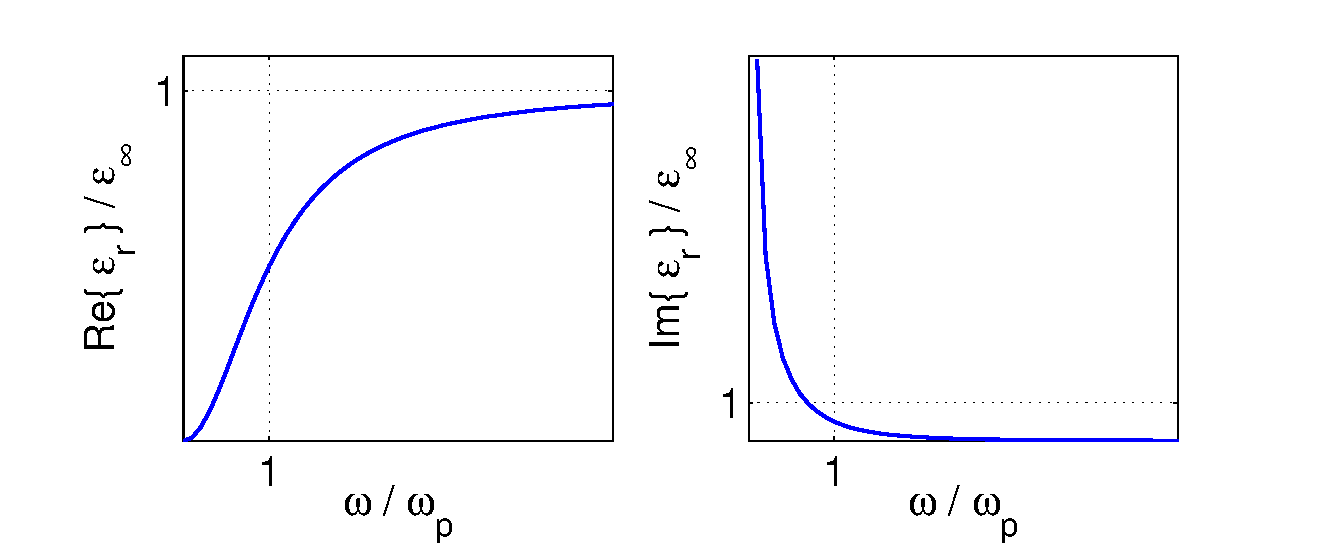
\includegraphics[scale=0.7]{Figures/Chapters/PhysicalProblem/drudePermittivity}
  \end{center}
  \caption{The real (left) and imaginary (right) parts of the dispersive
    frequency domain relative permittivity, $\hat{\eps}_r$, as obtained from
    Drude model.}
  \label{fig:read-and-imag-effective-permittivity}
\end{figure}


%%%%%%%%%%%%%%%%%%%%%%%%%%%%%%%%%%%%%%%%%%%%%%%%%%%%%%%%%%%%%%%%%%%%%%%%%%%%%%%%%%%%%%%%%%%%%%%%%%%%%%%%%%%%%%%%%%%%%%%%%%%%%%%%%%%%%%%%%%%%%%%%%%%%%
% More Dude Model Stuff
%%%%%%%%%%%%%%%%%%%%%%%%%%%%%%%%%%%%%%%%%%%%%%%%%%%%%%%%%%%%%%%%%%%%%%%%%%%%%%%%%%%%%%%%%%%%%%%%%%%%%%%%%%%%%%%%%%%%%%%%%%%%%%%%%%%%%%%%%%%%%%%%%%%%%
%
% TODO - direct quote - IntriaPaper DGTD dispersive
%
% When subjected to a constant external electric field $\Etilde$ the
% displacement of the heavy valence ions from their equilibtrium position is
% assume to be negligable whilst the electrons move significantly from their
% equilibrium position in response to an externally applied field. This results
% in an additional electric field $\Ptilde$ due to material response to the
% applied field $\Etilde$ orientated in the opposite direction resulting in a
% total field given by the electric displacement field $\Dtilde$ where:
% 
%  $$
%  \Dtilde = \eps_0 \Etilde + \Ptilde
%  $$
% 
%  Note that usually the signs of $\Ptilde$ and $\Etilde$ will be opposite -
%  resulting in an induced field that opposes the applied field and
%  consequentially a reduced field in the medium.
% 
%  %  TODO: Is it accurate to describe the displacement electric field as the
%  %  total electric field....?
% 
%  For a constant or slow-varying field with respect to the material response
%  time $\tau$ the polarisation of the material $\Ptilde$ will be proportional
%  to the applied electric field and can be described as a constant of
%  proportionality $\chi$, known as the electric susceptibility which describes
%  how susceptible the material is to polarisation. $\Ptilde$ can be written as:
% 
%  $$
%  \Ptilde = \chi \Etilde
%  $$
% 
%  $\chi$ is not always constant - and in general is a tensor.
% 
%  Furthermore the movement of electrons from their zero-field equlibrium
%  positions to the equilibrium positions under the applied field $\Etilde$
%  could take some finite time $\tau$ (characteristic time). For an applied
%  electric field $\Etilde$ which is changing sufficiently quickly this time
%  needs to be accounted for and $\chi$ may not be described as simply by a
%  constant since it clearly depends on the history of the mediums polarisation.
% 
%  TODO - derivation from equations of motion to conservation form....find a
%  nice way of doing this....
%
%
%
%  Even More Dude Model Stuff
%%%
%%%  Consider a medium under a constant external electric field $\Etilde$. Free
%%%  charged particles or charge dipoles in a material are subject to an applied
%%%  force. The equilibrium position of positive and negative charges will be
%%%  different to zero-field equilibrium positions and a net dipole moment, and
%%%  consequentially an electric field, is established. The electric
%%%  displacement, $D$, has a contribution due to polarisation of the material,
%%%  $P$, and~\eqref{eq:contitutive-linear-non-dispersive-1} is modified as
%%%
%%%   $$
%%%   \Dtilde(\mathbf{r},\ttilde) = \eps \Etilde(\mathbf{r},\ttilde) +
%%%   \Ptilde(\mathbf{r},\ttilde) ,
%%%   $$
%%%
%%%   In a changing applied field the movement of charges from a previous
%%%   equlibrium state to a subsequent equilibrium state could take some finite
%%%   time. Since this depends on the current state of polarisation the time
%%%   required to reach a new polarisation state is dependent not only on the
%%%   current applied field but also the history of the polarisation of the
%%%   medium. The material polarisation field $P$ can be written as
%%%
%%%   \begin{equation}
%%%   \Ptilde(\mathbf{r},\ttilde) = \eps_0 \int_{-\infty}^{+\infty} d \mathbf{r}' \int_{-\infty}^{\ttilde} dt' \chi (\mathbf{r} - \mathbf{r}', \ttilde - \ttilde') \cdot \Etilde(\mathbf{r}', \ttilde')
%%%   \label{eq:dispersive-convolution-integral}
%%%   \end{equation}
%%%
%%%
%%%   In the time domain the constitutive equations for dispersive materials
%%%   become non-local in time. The problem can be treated more naturally in the
%%%   frequency domain, where the material response depends on the applied
%%%   frequency. Then~\eqref{eq:contitutive-linear-non-dispersive-1} can be
%%%   written as:
%%%
%%%   \begin{equation}
%%%     \Dtilde(\omega) = \eps(\omega) \Etilde
%%%   \end{equation}
%%%
%%%
\section{Dimensionless form}

% "\eps_0 and \mu_0 introduces an arbitraryness of dimension which we exploit
% for the dimensionless form"
Maxwell's equations are not invariant under change of units, with the constants
$\eps_0$, $\mu_0$ and changing value and position. Unit systems in common
use include the SI units used above, Gaussian units, Lorentz-Heaviside units and
Planck units. In particular, for numerical simulations, a dimensionless unit
system is commonly used to avoid rounding errors in floating point arithmetic.
Maxwell's equations can be obtained in dimensionless form by scaling length and
time by an arbitrary characteristic length, $L$. The following changes of
variable are introduced:
\begin{align}
  \label{eq:dimensionless-scaling-1}
  \xbf &= \frac{\xbftilde}{\charLen}, &  \
                                        t &= \frac{\czero \ttilde}{\charLen}, &  \
                                                                           \plasfreq &= \frac{\plasfreqtilde \charLen}{\czero}, & \
                                                                                                                                  \gamma &= \frac{\gammatilde \charLen}{\czero},
\end{align}
where $\czero = ( \eps_0 \mu_0 )^{-\frac{1}{2}}$ is the speed of light in vacuum
in SI units, and the quantities $\xbf$ and $\t$ have been chosen such that the
dimensionless speed of light in vacuum is unity. Additionally, electromagnetic
field strengths and currents may be scaled by a characteristic field strength,
$\E_0$, by introducing the following dimensionless variables:
\begin{align}
  \label{eq:dimensionless-scaling-2}
  \E &= \Etilde, &  \
                   \H &= \intImpFS \Htilde, &  \
                                              \J &= \charLen \intImpFS \Jtilde, & \
                                                                                  \J_p &= \charLen \intImpFS \Jtilde_p,
\end{align}
% note - could also scale all of these values with E_0
where $\eta_0 = \sqrt{\mu_0 / \eps_0}$ is the intrinsic impedence of free space.
Derivatives with respect to $\ttilde$ and $\xbftilde$ are transformed as
\begin{align}
  \label{eq:dimensionless-scaling-3}
  \dpartttilde{\Box} &= \frac{\czero}{\charLen}\dpartt{\Box}, & \
                                                        \dpartxtilde{\Box} &= \frac{1}{\charLen}\dpartx{\Box}
\end{align}
By substitution of~\eqref{eq:dimensionless-scaling-1}
and~\eqref{eq:dimensionless-scaling-2} into Maxwell's curl
equations,~\eqref{eq:maxwell-ampere} and~\eqref{eq:maxwell-faraday}, we obtain
the curl equations modified for dispersive materials in dimensionless form:
\begin{subequations}
  \label{eq:dimensionless-maxwell}
  \begin{align}
    \nabla \times \E(\xbf,\t) + \dpartt{\B(\xbf, \t) } &= 0, \\
    \nabla \times \H(\xbf,\t) - \dpartt{ \D_{\infty}(\xbf, \t) } &= \J(\xbf,\t) - \J_p(\xbf,\t), \\
    \D_{\infty}(\xbf,\t) &= \eps_{\infty}(\xbf) \E(\xbf,\t), \\
    \B(\xbf,\t) &= \mu_r(\xbf) \H(\xbf,\t), \\
    \frac{d \J_p(\xbf,\t)}{d\t} + \gamma \J_p(\xbf,\t) &= - \omega_p^2 \E(\xbf,\t),
  \end{align}
\end{subequations}
where $\DInf$ and $\B$ are the appropriately scaled values of
$\DtildeInf$ and $\Btilde$.
Note that the non-dispersive form may be recovered in
the infinite frequency limit, where $\J_p = 0$, $\eps_{\infty} = \eps_r$
and $\DInf = \D$
equations,~\eqref{eq:maxwells-equations-diff}, to obtain the equivalent
non-dispersive dimensionless form.

\section{Conservation form}

% *** EVERYTHING WRITTEN AS FREE SPACE - \mu = 1 probably ok for my examples but
% \eps != 1 ***
The dispersive form of Maxwell's equations in dimensionless
form,~\eqref{eq:dimensionless-maxwell}, can be conveniently rewritten as a
linear, hyperbolic conservation law\cite{Godlewski:2013tj,LeVeque:2002vc}
% TODO - Ruben: need to show that system is hyperbolic (and linear?)
\begin{equation}
  \dpartt{ \, \USoltn} + \sum_{k=1}^{nsd} \frac { \partial \, \Flux_k(\USoltn) }{ \partial x_k } = \maxwellSource\,(\USoltn) \: ,
  \label{eq:maxwell-curl-equations-conservation-form}
\end{equation}
where $nsd$ denotes the number of spatial dimensions. The vector of unknowns,
$\USoltn$, the flux vectors, $\Flux_k$, and the source $\maxwellSource$ are
given by
\begin{equation*}
  \begin{array}{c}
    \USoltn =
    \begin{pmatrix}
      \eps_{\infty} E_1, \: \eps_{\infty} E_2 , \: \eps_{\infty} E_3 , \: \mu
      H_1 , \: \mu H_2 , \: \mu H_3 , \: J^p_1 , \: J^p_2 , \: J^p_3
    \end{pmatrix}^T,
    \\
    \Flux_1 =
    \begin{pmatrix}
      0 ,\: H_3 ,\: -H_2 ,\: 0 ,\: -E_3 ,\: E_2 ,\: 0 ,\: 0 ,\: 0
    \end{pmatrix}^T , \\

    \Flux_2 =
    \begin{pmatrix}
      - H_3 ,\: 0 ,\: H_1 ,\: E_3 ,\: 0 ,\: -E_1 ,\: 0 ,\: 0 ,\: 0
    \end{pmatrix}^T , \\

    \Flux_3 =
    \begin{pmatrix}
      H_2 ,\: -H_1 ,\: 0 ,\: -E_2 ,\: E_1 ,\: 0 ,\: 0 ,\: 0 ,\: 0
    \end{pmatrix}^T , \\

    \maxwellSource =
    \begin{pmatrix}
      J_1 + J^p_1 ,\: J_2 + J^p_2 ,\: J_3 + J^p_3 ,\: 0 ,\: 0 ,\: 0 ,\: \omega^2
      \: E_1 - \gamma J^p_1 ,\: \omega^2 \: E_2 - \gamma J^p_2 ,\: \omega^2 \:
      E_3 - \gamma J^p_3
    \end{pmatrix}^T,

  \end{array}
\end{equation*}

where $E_k$, $H_k$ and $J^p_k$ are the $k$th spatial components of the
dimensionless intensity vectors of electric field, magnetic field and the
polarisation current, respectively. The material parameters $\eps$, $\mu$,
$\omega$ and $\gamma$ are the electric permittivity, magnetic permeability,
plasma frequency and electron damping coefficient, respectively. The same form
may be used for non-dispersive cases, by setting $J^p_k = 0 \; \forall \; k$ and
setting $\eps_{\infty} = \eps_{r}$. The equations can be written in quasilinear form
\begin{equation}
  \label{eq:1}
  \dpartt{\USoltn}  + \AQuasiLinear_k\dpart{\xbf_k}{\USoltn} = \AQuasiLinear_s \USoltn  \;\;\;k = 1...\nsd
\end{equation}
where, in three dimensions

\begin{align}
\AQuasiLinear_k = 
    \begin{pmatrix}
      \zerov & \RQuasiL_{k} & \zerov \\
      -\RQuasiL_{k} & \zerov & \zerov \\
      \zerov & \zerov & \zerov \\
    \end{pmatrix}
  \: \:
\textrm{and}\;\;\;
\AQuasiLinear_s = 
    \begin{pmatrix}
      \zerov  & \zerov & -\IdentityVect\\
      \zerov & \zerov & \zerov \\
      -\plasfreq \IdentityVect & \zerov & - \gamma \IdentityVect \\
    \end{pmatrix}
\end{align}
with
\begin{align}
\RQuasiL_1 = 
    \begin{pmatrix}
      0 & 0 & 0 \\
      0 & 0 & 1 \\
      0 & -1 & 0 \\
    \end{pmatrix} ,
  \: \:
  &
\RQuasiL_2 = 
    \begin{pmatrix}
      0 & 0 & -1 \\
      0 & 0 & 0 \\
      1 & 0 & 0 \\
    \end{pmatrix}
  &
  \textrm{and   } \:\:\:
  &
\RQuasiL_3 = 
    \begin{pmatrix}
      0 & 1 & 0 \\
      -1 & 0 & 0 \\
      0 & 0 & 0 \\
    \end{pmatrix}
  &
\end{align}

% TODO - quasilinear form for TE and TM

\section{Reduction to 2 dimensions}
\subsection{TE and TM modes}
For a physical system where the electric field is translationally invariant in
the $z$-direction, the derivatives with respect to $z$ are zero. Maxwell's
equations are decoupled into two sets of coupled equations with three unknowns
each. The resulting modes in dimensionless form, accounting for dispersion with
the Drude model, are known as the $TE_z$ mode, given by

\begin{equation*}
  \begin{array}{ccccc}
    \USoltn_1 = \begin{pmatrix} \eps E_1 \\ \eps E_2 \\ \mu H_3 \\ J^p_1 \\  J^p_2 \end{pmatrix} ,
 &
   \Flux_1 = \begin{pmatrix} 0 \\ H_3 \\ E_2 \\ 0 \\  0 \end{pmatrix} ,
 &
   \Flux_2 = \begin{pmatrix} - H_3 \\ 0 \\ -E_1 \\ 0 \\ 0 \end{pmatrix} ,
 &
   \maxwellSource = \begin{pmatrix} J_1 + J^p_1 \\ J_2+ J^p_2 \\ 0 \\ \omega^2 \, E_1 - \gamma J^p_1 \\  \omega^2 \, E_2 - \gamma J^p_2 \end{pmatrix} ,
  \end{array}
  \:
\end{equation*}

and the $TM_z$ mode, given by

\begin{equation*}
  \begin{array}{ccccc}
    \USoltn = \begin{pmatrix} \eps E_3 \\ \mu H_1 \\ \mu H_2 \\ J^p_3 \end{pmatrix} ,
 &
   \Flux_1 = \begin{pmatrix} -H_2 \\ 0 \\ -E_3 \\ 0 \end{pmatrix} ,
 &
   \Flux_2 = \begin{pmatrix} H_1 \\ E_3 \\ 0 \\ 0 \end{pmatrix} ,
 &
   \maxwellSource = \begin{pmatrix} J_3 + J^p_3 \\ 0 \\ 0 \\ \omega^2 \, E_3 - \gamma J^p_3 \end{pmatrix} .
  \end{array}
  \:
\end{equation*}

In particular, radiation which is quantised by confinement in a waveguide can be
described by the $TE_z$ or $TM_z$ modes.
% In practice a system which can be approximated as having infinite extent in
% one direction can be approximated by a translationally invariant electric
% field in one direction.

\subsection{2D compact form}

Several physical systems, notably wave guides, may have known modal dependence
in a given direction. The compact form of Maxwell's equations was introduced by
Xiao\cite{Xiao:1992be} to allow a full wave analysis of Maxwell's equations in
waveguides using only a 2-dimensional mesh. The variation of fields in the
$z$-direction is assumed to be of the form
\begin{equation}
  \USoltn(x_1,x_2,x_3) = \USoltn_{12}(x_1, x_2,t) e^{-i \beta_z x_3},
  \label{eq:compact2D-zdep}
\end{equation}
where $\beta_z$ is the wave propagation constant in the $z$-direction. By
substitution into Maxwell's non-dispersive
equations,~\eqref{eq:maxwell-curl-equations-conservation-form}, with
$\maxwellSource = 0$, the system of equations obtained can be written in compact
form\cite{}, resulting in the following expressions for $\USoltn$,$\Flux_{k}$
and $\maxwellSource$
\begin{equation*}
  \begin{array}{ccccc}
    \USoltn = \begin{pmatrix} \eps_{\infty} E_1 \\ \eps_{\infty} E_2 \\ \eps_{\infty} E_3 \\ \mu H_1 \\ \mu H_2 \\  \mu H_3  \end{pmatrix} ,
 &
   \Flux_1 = \begin{pmatrix} 0 \\ H_3 \\ -H_2 \\ 0 \\ -E_3 \\ E_2  \end{pmatrix} ,
 &
   \Flux_2 = \begin{pmatrix} - H_3 \\ 0 \\ H_1 \\ E_3 \\ 0 \\ -E_1 \end{pmatrix} ,
 &
   \maxwellSource = \begin{pmatrix} H_2 \\ -H_1 \\ 0 \\ -E_2 \\ E_1 \\ 0 \end{pmatrix} i \beta_z ,
  \end{array}
  \:
\end{equation*}

where the fields $E_k'$, $H_k'$ do not contain any dependence on $z$. Note that
the expression for $\maxwellSource$ is now complex, however for scalar permittivities the system can be solved by taking only
the real part\cite{zhao1997relationship,pile2005compact}.
% TODO - Ruben : the citations here might need to be changed
%
% E Blank In case a numerical scheme is applied to discretize the curl-equations, the divergence
% conditions do not have to be fulfilled automatically, as was pointed out in
% e.g. Ref. [36]. It might be necessary to design a scheme that takes the
% divergence constraints numerically into account, as suggested in Ref. [37],
% where a Discontinuous Galerkin Method is applied to Maxwell’s equations using
% a locally divergence-free
Note that when $\beta_z = 0$ this decouples into the $TE_z$ and $TM_z$ modes as
expected since in this case there is no $z$-dependence.



% E Blank In case a numerical scheme is applied to discretize the
% curl-equations, the divergence conditions do not have to be fulfilled
% automatically, as was pointed out in e.g. Ref. [36]. It might be necessary to
% design a scheme that takes the divergence constraints numerically into
% account, as suggested in Ref. [37], where a Discontinuous Galerkin Method is
% applied to Maxwell’s equations using a locally divergence-free
%

% $$ \pdert{E_1} = \pder[H_{3}]{x_2} - \pder[H_{2}]{x_3} $$
% $$ \pdert{E_2} = \pder[H_{1}]{x_3} - \pder[H_{3}]{x_1} $$
% $$ \pdert{E_3} = \pder[H_{2}]{x_1} - \pder[H_{1}]{x_2} $$
% $$ \pdert{H_1} = - \pder[E_{3}]{x_2} + \pder[E_{2}]{x_3} $$
% $$ \pdert{H_2} = - \pder[E_{1}]{x_3} + \pder[E_{3}]{x_1} $$
% $$ \pdert{H_3} = - \pder[E_{2}]{x_1} + \pder[E_{1}]{x_2} $$
% 
% The system of equations can be written in 3D as a linear hyperbolic system of
% conservation equations:
% 
% $$
% \pder[\USoltn]{t} + \pder[\Flux_k(\USoltn)]{x_k} = \maxwellSource(\USoltn)
% $$
% 
% where:
% 
% $$
% \USoltn = \begin{pmatrix}\eps \E \\ \mu \H \end{pmatrix} \mathbf{F_1}
% = \begin{pmatrix}0 \\ H_3 \\ - H_2 \\ 0 \\ - E_3 \\ E_2 \end{pmatrix}
% \mathbf{F_2} = \begin{pmatrix} -H_3 \\ 0 \\ H_1 \\ E_3 \\ 0 \\ -
%   E_1 \end{pmatrix} \mathbf{F_3} = \begin{pmatrix} H_3 \\ -H_1 \\ 0 \\ -E_2 \\
%   E_1 \\ 0 \end{pmatrix} \maxwellSource = \mathbf{0}
% $$
% 
% We can approximate the z-dependence of the system as a sinusoidal wave where
% each component of the system follows a sinusoidal $x_3$ dependence given by:
% 
% $$
% \USoltn(x,y,z) = \USoltn(x,y) e^{j(\beta t - \omega t)}
% $$
% 
% The system of equations can be reduced to 2D by specifying an explicit form
% for $F_3$. The equation above is therefore modified to have only $F_1$ and
% $F_2$ with an explicit form for $\pder{F_3}$ introduced as a source term of
% form.
% 
% $$
% \maxwellSource = \begin{pmatrix} \beta sin(\omega t - \beta x_3) \\ \beta
%   sin(\omega t - \beta x_3) \\ 0 \\ \beta sin(\omega t - \beta x_3) \\ \beta
%   sin(\omega t - \beta x_3) \\ 0 \end{pmatrix}
% $$


\section{Interfaces}
% $$
% \mathbf{n} \times \mathbf{E^L} = \mathbf{n} \times \mathbf{E^R} \mathbf{n}
% \times \mathbf{H^L} = \mathbf{n} \times \mathbf{H^R}
% $$
% 
% $$
% \mathbf{n} \cdot ( \eps^L \mathbf{E^L} ) = - \mathbf{n} \cdot ( \eps^R
% \mathbf{E^R} )
% $$
% $$
% \mathbf{n} \cdot ( \mu^L \mathbf{H^L} ) = - \mathbf{n} \cdot ( mu^R
% \mathbf{H^R} )
% $$
%
% TODO - note in Rubens thesis the last equation contains \eps^R\H^R (is this
% correct?)


\subsection{Normal fields}

Consider an interface between two materials, where the material parameters
$\eps$ and $\mu$ change. On the left hand side of the interface we denote the
material parameters as $\eps_L$ and $\mu_L$, and on the right hand side as
$\eps_R$ and $\mu_R$. On the interface, the values of the fields may be
discontinuous, and the differential forms of Maxwell's equations may not be
valid. However interface conditions relating the field values on either side of
the interface, can be derived from the integral form.

Let $E_L$ and $E_R$ be values of the electric field, $E$, in the limit of
approaching the interface from the left or right respectively. Let $S$ be a
cylindrical closed surface, of height $h$, which encloses part of a planar
interface, $I$, where the parallel planes of $S$ are parallel to the interface,
as shown in Figure \ref{fig:material-interface-derivation:E-pillbox}. The
surface of the interface $I$, enclosed by $S$ is denoted as $\Delta I$.
\begin{figure}[htbp!]
  \begin{center}
    \includegraphics[height=0.3\textheight]{Figures/Chapters/PhysicalProblem/interfaceEPillBox}
  \end{center}
  \caption{Schematic showing integration surfaces used to obtain conditions for
    normal fields across an material interface.}
  \label{fig:material-interface-derivation:E-pillbox}
\end{figure}
In the limit $h \to 0$, all electric flux leaves the volume through the parallel
planes of the surface $S$, and~\eqref{eq:maxwell-gauss-integral} can be written
as
$$
\D_L \cdot \hat{\mathbf{n}} \Delta I - \mathbf{D}_R \cdot \hat{\mathbf{n}}
\Delta I = \rho_s \Delta I,
$$
where we have assumed that $S$ is sufficiently small that $D$ is constant. The
material interface condition can be written as
$$
\D_L \cdot \hat{\mathbf{n}} - \mathbf{D}_R \cdot \hat{\mathbf{n}} = \rho_s .
$$
Note that in the case where $\rho_s = 0$, meaning that there are no free
(unbound) charges, then the normal component of the electric flux density, $D$,
is continuous across the interface. By following the analogous procedure for the
magnetic field using~\eqref{eq:maxwell-gauss-magnetism-integral} we obtain
$$
\B_L \cdot \hat{\mathbf{n}} = \B_R \cdot \hat{\mathbf{n}} .
$$
These conditions are used with Maxwell's divergence equations.
% not used in the code!?

\subsection{Tangental fields}

Similarily for the tangental component of electric field we consider a closed
rectangular integration path in the plane of $\E_L$ and $\E_R$ around the same
interface, as shown
in~\eqref{fig:material-interface-derivation:E-rectangular-loop}. Again in the
limit $h \to 0$ and noting that $d\maxwellSource = 0$, we can
write~\eqref{eq:maxwell-faraday-integral} as
\begin{figure}[htbp!]
  \begin{center}
    \includegraphics[height=0.3\textheight]{Figures/Chapters/PhysicalProblem/interfaceContour}
  \end{center}
  \caption{Schematic showing integration contours used to obtain conditions for
    tangental fields across an material interface.}
  \label{fig:material-interface-derivation:E-rectangular-loop}
\end{figure}
\begin{equation}
  \label{eq:material-interfaces-tangentalcondition-E}
  \int_{L_1}^{L_2} \E_L \cdot d\mathbf{l} - \int_{R_1}^{R_2} \E_R \cdot d \mathbf{l} = 0
\end{equation}
or
$$
\E_L \cdot d\mathbf{l} = \E_R \cdot d \mathbf{l} .
$$

The resulting interface condition is therefore that components of $\E$ tangental
to the interface are continuous - which can be written more generally as
$$
\hat{\mathbf{n}} \times \E_L = \hat{\mathbf{n}} \times \E_R .
$$
Again following an analogous procedure for the magnetic field we obtain
$$
\hat{\mathbf{n}} \cdot \H_L = \hat{\mathbf{n}} \times \H_R .
$$
These conditions are used with Maxwell's curl equations.

\subsection{Perfect electric conductors}
Metals with a large number of conduction band electrons can be described by the
perfect electric conductor (PEC) approximation. In a PEC the coulomb repulsion
between electrons causes all free charges to be distributed in an
infinitesimally thin layer on the surface of the material. The distribution of
free charges within a PEC changes instantaneously to counteract any applied
electric fields. Let us consider that the material on the right hand side of the
interface described above is a PEC. In this case, since $E_R$ is zero inside the
material, then~\eqref{eq:material-interfaces-tangentalcondition-E} simply
becomes
$$
\int_{L_1}^{L_2} \E_L \cdot d\mathbf{l} = 0 ,
$$
and the resulting condition is
$$
\E_L \times \hat{\mathbf{n}} = 0 .
$$
Similarily for the magnetic field we obtain
$$
\H_L \times \hat{\mathbf{n}} = \J_s ,
$$
% what about the other two conditions i.e. divergence conditions - should I
% specify those too?
where $\J_s$ is the surface current.

\subsection{Radiation condition}
Solution of many problems of interest require computation of phenomena occuring in a physical domain of infinite extent. In such a domain, electromagnetic sources should scatter energy to infinity. The inverse process, where radiation transfers energy from infinity to location of the sources is non-physical. To ensure uniqueness of solutions in an infinite domain, the following condition, known as the Silver-M\"uller radiation condition, should be satisfied
\begin{align}
\lim{ r \to \infty } \left( \xbf \times \left( \nabla \times \E \right) + \norm{\xbf} \dpartt{\E} \right) = 0, \\
\lim{ r \to \infty } \left( \xbf \times \left( \nabla \times \H \right) + \norm{\xbf} \dpartt{\H} \right) = 0.
\end{align}

\section{Relation to wave equation and Helmholtz equation}
\subsection{Wave equation}

Within a homogenous medium, where material parameters are constant and no free
currents or charges are present, Maxwell's equations can be written in wave
equation form, for which plane wave analytical solutions can be
obtained\cite{Jackson:490457}. By combining Faraday's law in SI
form,~\eqref{eq:maxwell-ampere}, with the appropriate constitutive equations for
non-dispersive media,~\eqref{eq:constitutive-linear}, we obtain the expression
\begin{equation}
  \label{eq:wave-equation-derivation-1}
  \nabla \times ( \nabla \times \H ) + \eps_0 \eps_r \dpartt{ \nabla \times \E } = 0 .
\end{equation}
where in the absence of free currents and charges we have used $\J = 0$ and
$\rho = 0$.

Subsituting both the vector identity $ \nabla \times ( \nabla \times \H ) = \nabla \cdot ( \nabla \cdot \H ) - \nabla^2 \H,
$
where we note from~\eqref{eq:maxwell-gauss-2} that $\nabla \cdot \H = 0$, and
Ampere's law,shown in~\eqref{eq:maxwell-ampere},
into~\eqref{eq:wave-equation-derivation-1} we obtain

\begin{equation}
  \label{eq:maxwell-wave-eqtn-H}
  \nabla^2 \H = \frac{1}{c^2} \ddpartt{ \H },
\end{equation}
which is a wave equation in the unknown $\H$, with the speed of the resultant wave given by $c_0 = 1/\sqrt{\eps_0 \eps_r \mu_0 \mu_r }$. We note that
the quantities $\eps_0$ and $\mu_0$ are related to the speed of light 
in vacuum $c_0 = 1/\sqrt{\eps_0 \mu_0 }$. A similar procedure can be followed, starting from
Ampere's law, leading to
\begin{equation}
  \label{eq:maxwell-wave-eqtn-E}
  \nabla^2 \E = \frac{1}{c^2} \ddpartt{ \E } .
\end{equation}
% TODO - Ruben : comments are missing - what are the advantages/limitations of
% this formulation!! Look at LeVeque - why do we use conservation laws in this
% way?

\subsection{Helmholtz equation}
The Helmholtz or reduced wave equation form of~\eqref{eq:maxwell-wave-eqtn-E} is
of particular interest for frequency domain numerical simulations. In this
approach the fields $\E$ and $\H$ are assumed to be time-harmonic, and are
expressed as
\begin{align}
  \label{eq:maxwell-helmholtz-time-harmonic}
  \E(\xbf,t) = \Re \left( \EHelm(\xbf) e^{i \omega t} \right), \\
  \H(\xbf,t) = \Re \left( \HHelm(\xbf) e^{i \omega t} \right),
\end{align}

which, by substitution into the wave equations given
in~\eqref{eq:maxwell-wave-eqtn-E} and~\eqref{eq:maxwell-wave-eqtn-H} we obtain
the Helmholtz equations for electric and magnetic fields
\begin{align}
  \label{eq:helmholtz}
  \nabla^2 \E(\xbf) + k^2 \E(\xbf) = 0, \\
  \nabla^2 \H(\xbf) + k^2 \H(\xbf) = 0,
\end{align}
where $k^2 =\omega^2/c^2$, is known as the propagation constant.

In this form the equations for $\E$ and $\H$ can be solved independently for
each angular frequency, $\omega$. This approached is best suited
to problems with a small number of frequencies of interest, for example a system
which is being driven at a known frequency. By contrast time domain approaches
allow solution for a broad band of frequency responses at once.


% TODO Balanis citation is incomplete P Drude - needs to be removed - maybe the
% solid state one (Optical properties of solids) instead Maybe swap some of the
% references for others (e.g. Fox) Ruben made LOADS of comments on citations Use
% some citations from Rubens paper also


%%% Local Variables:
%%% mode: latex
%%% TeX-master: "../Thesis"
%%% End:

%\chapter{Discontinuous Galerkin Method for Maxwells Equations} % Write in your own chapter title
\label{Chapter3}
\lhead{Chapter 3. \emph{Discontinuous Galerkin}} % Write in your own chapter title to set the page header

The Discontinuous Galerkin method was first introduced to solve the neutron transport problem by Reed and Hill \cite{} in 1973.
** Some background/literature review here Cockburn, Shui for solving hyperbolic equations etc ***
% PhDJesusAlvarez good for motivation - not so much for the method

As seen in Chapter~\ref{PhysicalProblemChapter}, given a suitable choice of
initial conditions the evolution of the system in time can be described by
Maxwell's curl equations in strong
form,~\eqref{eq:maxwell-curl-equations-conservation-form}. Consider that the problem is defined on an open bounded physical domain, $\physicalDomain \in \Real^{\nsd}$, with a boundary $\physicalDomainBoundary$,
% TODO - should I specify that its a PEC boundary (Ruben does)
which is partitioned in an unstructured mesh of $\nel$ nonoverlapping, body-conforming simplices, $\elemIndexed$, such that
$$
\bar{\physicalDomain} = \mathop{\bigcup}_{\elemindex=1}^{\nel} \barelemindexed, \;\; \elemIndexed \cap \anotherelem \textrm{for} \elemindex \neq \anotherelemindex
$$.
% TODO - no approx here...!? Understand why this is...

% discuss the discretisation more - duplication of nodes?
Following the method of weighted residuals for a single element we seek solutions to the strong form problem,~\eqref{eq:maxwell-curl-equations-conservation-form}, over a generic element, $\genericElement$, in the approximation space $\left( \E,\H,\J \right) \in \approximationSpaceTotal \left( \left[ 0, \periodOfApproximation \right], \approximationSpaceSpatial \right)$
% TODO - check WHICH J I'm using here
where $\approximationSpaceSpatial = \spaceOfSpatialApproximationFunction $ with
% TODO - more space approx stuff here.
Multiplied by a vector of test functions $\TF \in \approximationSpaceSpatial $ and integrated over the generic element $\elemIndexed$ results in,
$$
\int_{\genericElement} \TF \cdot \uet \delem  + \int_{\genericElement} \TF \cdot \dpart{\Flux_{k}}{x_{k}}= \int_{\genericElement} \TF \cdot \maxwellSource \delem,
$$
where $\Ue$ denotes the restriction of $\USoltn$ to the element $\genericElement$ and einsteins summation notation has been employed.
% TODO - is this technically true
Integration by parts results in

\begin{equation}
\int_{\genericElement} \TF \cdot \uet \delem  - \int_{\genericElement} \dpart{\TF}{\xk} \cdot
\Flux_{k}(\Ue) \delem + \int_{\genericElementtrace} \TF \cdot \NormalFlux(\Ue) \delemtrace
= \int_{\genericElement} \TF \cdot \maxwellSource(\Ue) \delem,
\label{eq:weak-form-with-physical-flux}
\end{equation}

where $\outnormalvector$ is outward unit normal vector to the boundary $\genericElementtracegenericelement$ of $\genericElement$, which has directional cosines $\outnormalcoeffk$, and $\mathbf{F_n}$ is the outward normal physical flux, given by $ \mathbf{F_n}(\mathbf{U}) = \outnormalcoeffk \mathbf{F}_k(\mathbf{U}) $.

Since the weak form stated in~\eqref{eq:weak-form-with-physical-flux} is specified on the element $\genericElement$, this does not constitute a scheme suitable for solving the global problem. As is usual in a DG context, continuity of the solution between elements is weakly enforcing by replacing the physical normal flux, $\NormalFlux(\Ue)$, with a consistent numerical flux, $\NumFlux(\Ue,\Uout)$. This numerical flux depends on both the trace of the solution on the element $\genericElement$ and the trace of the solution on the neighbouring element, $\mathbf{U}^{out}$.
% TODO: What is the definition of Uout in mathematical language ??
For a linear hyperbolic system a natural choice is to employ a flux splitting technique~\cite{donea2003finite}, corresponding to an upwind approximation\cite{chen2005high}.
% TODO: this is a lot like Rubens/Obays paper, rewrite it. QUOTE: A natural choice, for the linear hyperbolic system of interest here, is to employ a flux splitting technique ~\cite{donea2003finite}, which corresponds to an upwind approximation \cite{chen2005high}
The physical normal flux is written as
$$
\NormalFlux(\USoltn) = \An \USoltn,
$$
where $\An = \outnormalcoeffk \Ak$, and decomposed into incoming (superscript -) flux and outgoing flux (superscript +) as
% VIVA: An is known as the jacobian matrix, and apparently is also \An = \frac{ \partial \NumFlux }{ \partial \U }
\begin{align}
\NormalFlux(\USoltn) = \NormalFluxPositiveEigenvalues(\USoltn) + \NormalFluxNegativeEigenvalues(\USoltn),
\label{eq:phys-flux-splitting}
\end{align}
where $ \NormalFluxPositiveEigenvalues = \AnPlus \USoltn$, $\NormalFluxNegativeEigenvalues = \AnMinus \USoltn, $ and the matrices $\AnMinus$ and $\AnPlus$ denote respectively the matrices of the positive and negative eigenvalues of $\An$. These can be written conveniently as
\begin{align}
  \label{eq:AnMinus-AnPlus-Definition}
\AnPlus &= \left( \An + \AnMod \right) / 2   \\
\AnMinus &= \left( \An - \AnMod \right) / 2
\end{align}
where %TODO: definition of AnMod and change AnMod to another symbol...Add the definition of An...
The choice of an upwind approximation results in
\begin{align}
\NumFlux(\USoltn) = \NormalFluxPositiveEigenvalues(\USoltn) + \NormalFluxNegativeEigenvalues(\Uout).
\label{eq:num-flux-splitting}
\end{align}
After substitution of $\NumFlux$ and integration by parts,~\eqref{eq:weak-form-with-physical-flux} becomes
\begin{align*}
\int_{\elem} \TF \cdot \uet \delem  + \int_{\elem} \TF \cdot \dpart{\Flux_{k}(\Ue)}{\xk} \delem + \int_{\elemtrace} \TF \cdot \left[ \NumFlux(\Ue,\Uout) - \NormalFlux(\Ue) \right] \delemtrace \\
= \int_{\elem} \TF  \cdot \maxwellSource(\Ue) \delem, \label{eq:weak-form-upwind-splitting-fluxes}
% the second term changes from + to - from prev weak form
\end{align*}
We note that % TODO - I've lost some text here...!
\begin{equation}
  \NumFlux(\Ue,\Uout) - \NormalFlux(\Ue) = \AnMinus \Uout - \AnMinus \USoltn = \AnMinusU, \label{eq:AnMinusUderivation}
\end{equation}
where $\JumpU = \Uout - \USoltn$ denotes the jump in the solution across $\elemtracegenericelement$. By substitution into~\eqref{eq:weak-form-upwind-splitting-fluxes}, the weak form with upwind flux splitting is written as
\begin{equation}
\int_{\elem} \TF \cdot \uet \delem  + \int_{\elem} \TF \cdot \dpart{\Flux_{k}(\Ue)}{\xk} \delem + \int_{\elemtrace} \TF \cdot \AnMinusU \delemtrace = \int_{\elem} \TF  \cdot \maxwellSource(\Ue) \delem,
\label{eq:weak-form-final}
\end{equation}

% TODO: missing some stuff on diagonalisation of A here....is it necessary, also the form of the
% positive and negative eigenvalues.
% TODO: Missing the form of the numerical flux for DG!!
% *** conditions to be satisfied by numerical flux + form of numerical flux ***
% TODO: upwind flux: effect for wave domination problems - flow of information, upwind flux

\section{Internal Element Boundaries}
We consider the boundary conditions at an internal boundary between elements. From~\ref{sec:conservation-form}, this expression may be written as
$$
  \An =
  \begin{pmatrix}
 & \zerom , & \mu^{-1} \RTotNorm, & \zerom \\
 & - \eps^{-1} \RTotNorm & \zerom & \zerom \\
 & \zerom & \zerom & \zerom 
 & \end{pmatrix} ,
$$
where
$$
  \RTotNorm =
  \begin{pmatrix}
 & 0 & n_3 & -n_2 \\
 & -n_3 & 0 & n_1 \\
& n_2 & -n_1 & 0 
 & \end{pmatrix} .
$$
The modulus of $\An$ is then given by
\begin{align*}
\AnMod = \speedoflight
\begin{pmatrix}
  \modAnSubMatrix & \zerom & \zerom \\
  \zerom  & \modAnSubMatrix & \zerom \\
   \zerom & \zerom & \zerom 
\end{pmatrix}
\end{align*}
where $\speedoflight = \left( \eps \mu  \right)^{-\frac{1}{2}}$ is the speed of light in the medium and
\begin{align*}
  \modAnSubMatrix = 
\begin{pmatrix}
\outnormalcoeff_2^2 + \outnormalcoeff_3^2 &      -\outnormalcoeff_1 \outnormalcoeff_2 &      -\outnormalcoeff_1 \outnormalcoeff_3 \\
-\outnormalcoeff_1 \outnormalcoeff_2 & \outnormalcoeff_1^2 + \outnormalcoeff_3^2 &      -\outnormalcoeff_2 \outnormalcoeff_3 \\
-\outnormalcoeff_1 \outnormalcoeff_3 &      -\outnormalcoeff_2 \outnormalcoeff_3 & \outnormalcoeff_1^2 + \outnormalcoeff_2^2 \\
\end{pmatrix} ,
\end{align*}
where the identity $\sqrt{\sum_{\outnormalcoeffcomp} \outnormalcoeffk^2} = 1$, for the unit vector $\outnormalvector$, has been used. We therefore write
\begin{align*}
\AnMinus = \speedoflight
\begin{pmatrix}
  -\modAnSubMatrix & \RTotNorm & \zerom \\
  -\RTotNorm  & -\modAnSubMatrix & \zerom \\
   \zerom & \zerom & \zerom 
\end{pmatrix} .
\end{align*}

Noting that $\RTotNorm \anyVector = \outnormalvector \times \anyVector$ and $\modAnSubMatrix \anyVector = \outnormalvector \times \left(  \outnormalvector
  \times \anyVector \right)$,for any vector $\anyVector$, results in the expression
\begin{align}
\AnMinusU = \frac{1}{2}
\begin{pmatrix}
  -\nvect \times \left( \JumpH + \sqrt{\frac{\eps}{\mu}} \nvect \times \JumpE \right) \\
   \nvect \times \left( \JumpE + \sqrt{\frac{\mu}{\eps}} \nvect \times \JumpH \right) \\
  \zerov
\end{pmatrix} .
  \label{eq:AnMinuU-expression-3D}
\end{align}
% Should I write out A_n for the TEz and TMz modes?
A similar procedure results in
\begin{align}
\AnMinusU =
  \frac{1}{2}
  \left[
    \Jump{H_3} - \sqrt{\frac{\eps}{\mu}} \Jump{\alphaGeneral}
  \right]
\begin{pmatrix}
   -\outnormalcoeff_2 \\
   \outnormalcoeff_1 \\
   - \sqrt{ \frac{\mu}{\eps} } \\
   0  \\
   0 
\end{pmatrix} . \label{eq:AnMinuU-expression-TE}
\end{align}
with $ \alphaGeneral = n_1 E_2 - n_2 E_1. $ for the $\TEz$ mode and
\begin{align}
\AnMinusU =
  \frac{1}{2}
  \left[
    \Jump{E_3} - \sqrt{\frac{\mu}{\eps}} \Jump{\alphaGeneral}
  \right]
\begin{pmatrix}
   \outnormalcoeff_2 \\
   -\outnormalcoeff_1 \\
   -\sqrt{ \frac{\eps}{\mu} } \\
   0 
\end{pmatrix} . \label{eq:AnMinuU-expression-TM}
\end{align}
for the $\TMz$ mode with $ \alphaGeneral = - n_1 H_2 + n_2 H_1. $

% VIVA: calculated with matlab script:
% modAn = sqrtm(An*An') and knowing that
% make sure I can do sqrtm by hand
\section{Spatial Discretisation}
This section describes two approaches to spatial discretisation of the weak formulation~\ref{eq:weak-form-final}, namely the traditional isoparametric finite element formulation and the recently proposed NURBS-enhanced finite element method (NEFEM).

\section{Isoparametric Finite Element Method}
\label{sec:isoparametric-elements}
A nodal interpolation of the solution, $\USoltn$, is defined in a reference element $\refelem$, with local coordinates $\refElemCoords$, as
% TODO: do this directly in the 
\begin{align}
\USoltn_e(\xbf,\t) \simeq \sum_{j=1}^{\nen} \SF_{j} (\xbf) \UVect_{j}(\t) ,
\label{eq:nodal-basis-defn}
\end{align}
% TODO - copy this directly from Ruben Paper!! COPYRUBEN
% VIVA: the second U_j is the vector of coefficients
where $N_{j}$ are polynomial, Lagrangian shape functions of order $p$ in $\refElemCoords$ and $\nen$ are the number of nodes of the element $\meshelem$. An isoparametric transformation, $\IsoMapping$, is introduced between the reference element, $\refelem$ and a generic mesh element $\meshelem$, namely
% TODO - COPYRUBEN -> iso mapping - add comma to the end
where $\nodalCoordinatesOfElement$ are the nodal coordinates of the element $\meshelem$. Note that for an element with a face or edge on the boundary of the computational domain, the boundary of the element $\meshelem$ will be a polynomial approximation of the real boundary\cite{}.
% TODO - COPY RUBEN for citation
 Following the Galerkin method, the vector of test functions, $\TF$, is chosen from the same basis as the shape
functions.
Substitution of~\eqref{eq:nodal-basis-defn} into~\eqref{eq:weak-form-final}, and selecting the space of test functions to be the same as the space spanned by the approximation functions, results in the system
% NOTE - the second term actually also has an implicit sum over k in (Einstein notation)
$$
\discretisedWeakForm{\nfn}
\label{eq:discretised-weak-form-fem}
$$
% TODO - what is the ij subscript, and also why is the An taken out of the face matrix if it isn't constant over the face?
of $\nen$ ordinary differential equations, for each node $i$, where $\UVect_j$ is a vector of the solution coefficients at the $j$th node, $\MassMatrix$ is the elemental mass matrix, $\IdentityMatrix$ is the identity matrix, $\ConvectionMatrix$ is the convection matrix in the direction $x^{k}$, $\MassMatrixFace$ is the face mass matrix and $\nfn$ denotes the number of face nodes. Note that a choice of Lagrangian, nodal shape functions results in a block diagonal elemental mass matrix. Additionally, an isoparametric mapping results in the restriction of the index $\faceindex$ to face nodes only, since other terms are zero. These matrices are defined by
\begin{align*}
\MassMatrix &= \int_{\meshelem} \SF_i \SF_j \delem \\
\ConvectionMatrix &= \int_{\meshelem} \SF_i \dpart{\SF_j}{\xk}\delem \\
\MassMatrixFace &= \int_{\meshelemtrace} \SF_i \SF_j \delemtrace
\end{align*}
% TODO - why is Ruben as a captial here? And why is M_{ij} captial...none of this make sense...!
% TODO - why dont I change the integration element here?

Using the isoparametric mapping~\eqref{eq:isoparametric-mapping}, the integrals over $\meshelem$, are transformed to the reference element, $\refelem$, as
\begin{align*}
\MassMatrix &= \int_{\refelem} \SF_i \SF_j |\Jacobian| \delem \\
\ConvectionMatrix &= 
                               \sum_{l=1}^{\nsd}
                                \int_{\refelem} \SF_i
                               \Jacobian_{lk}^{-1}
                               \dpart{\SF_j}{\xi_{l}}
                             |\Jacobian|
                             \delem
\end{align*}
where $\Jacobian = \frac{\partial \phi}{ \partial \xi}$, is the Jacobian of the mapping $\IsoMapping$. Similarly, the face mass matrix is evaluated as
\begin{align*}
\MassMatrixFace &= \int_{\refelemtrace} \SF_i \SF_j || \JacobianFace || \delemtrace
\end{align*}
% TODO - double lines here around HJacobian Face A) insert them properly B) what are they??
where $\JacobianFace$ is the Jacobian of the restriction of the isoparametric mapping to the element face.

% Wikipedia: 'In geometry, an affine transformation, affine map[1] or an affinity (from the Latin, affinis, "connected with") is a function between affine spaces which preserves points, straight lines and planes.'
For elements for which the transformation $\IsoMapping$ is affine, both $\Jacobian$ and $\JacobianFace$ are scalar constants over the element, and therefore the elemental matrices simplify to
\begin{align*}
\MassMatrix &= |\Jacobian| \MassMatrixAffine \\
\ConvectionMatrix &= |\Jacobian|
                               \sum_{l=1}^{\nsd}
                               \Jacobian_{kl}^{-1}
                               \ConvectionMatrixAffine \\
\MassMatrixFace &= || \JacobianFace || \MassMatrixFaceAffine
,
\end{align*}
% TODO - double lines here around Jacobian Face
with the reference elemental matrices
\begin{align*}
\MassMatrixAffine &= \int_{\refelem} \SF_i \SF_j \drefelem \\
\ConvectionMatrixAffine &= \int_{\refelem} \SF_i
                             \left(
                               \dpart{\SF_j}{\xi_{l}}
                             \right)
                             \drefelem \\
\MassMatrixFaceAffine &= \int_{\refelemtrace} \SF_i \SF_j \delemtrace
,
\end{align*}
which depend only on the shape functions and the geometry of $\refelem$. The reference elemental matrices $\MassMatrixAffine$, $\ConvectionMatrixAffine$ and $\MassMatrixFaceAffine$ can be computed \textit{a priori} in the reference element, inverted if necessary and stored. Computation of $\ConvectionMatrix$, $\MassMatrixFace$ and the inverse of $\MassMatrix$ for each element therefore reduces to a multiplication of the reference element matrix by a scalar. Whenever possible meshes are constructed in order to maximise the number of elements for which an affine mapping can be established between $\refelem$ and $\meshelem$. For curved elements, since the $|\Jacobian|$ and $|\JacobianFace|$ are not constant, it is not possible to precompute reference element matrices. In practical applications however, meshes are constructed where with an extremely low number of curved elements. In these cases the elemental matrices $\MassMatrix$, $\ConvectionMatrix$ and $\MassMatrixFace$ are computed and stored once per element.
The resulting implementation, in which numerical integration is performed \textit{a priori}, is known as the \textit{quadrature-free} implementation\cite{DGPaper:42}, and can reduce the cost of a high-order DG method by a factor of 100\cite{DGPaper:41}.
% VIVA : no loop on gauss points now!!
% TODO / VIVA : what about factoring \AnMinu out of the integrand because n is constant over a planar face????
% TODO - also cite Rubens paper here: The use of hybrid meshes to improve the efficiency of a discontinuous Galerkin
% TODO - what is this whole thing with triangular/tetrahedral meshes -> always constant jacobian unless curved, Quads -> not always constant jacobian unless curved, should I elabourate?


% TODO - 'isoparametric mapping given by the coords of the vertices of Omega
%%%  In order to perform the integration over the element interior an isoparametric
%%% mapping, $\IsoMapping$, is introduced from a reference element $\refelem$ to the
%%% physical element $\elem$. The integrals in~\eqref{}, once transformed to the
%%% reference element, become
% TODO - ruben has lk not lk on Jacobian matrix
% VIVA - make sure I know what this definition of J means
% TODO - easier way of saying this
% TODO - comment (remark) on affine elements, and how I can remove the jcaobian etc etc




\section{NURBS-enhanced finite element method (NEFEM)}
% TODO - polynomial approximation of the boundary stuff here (take it from the paper maybe)
In the NEFEM approach, the approximation is defined directly in the physical space in Cartesian coordinates, as
\begin{align}
\USoltn_e(\xbf,\t) \simeq \USoltnApprox = \sum_{j=1}^{\nen} \SF_{j} (\xbf) \UVect_{j}(\t) ,
\label{eq:nodal-basis-defn}
\end{align}
% TODO - I haven't defined U_h here...!
% TODO - duplicate definition of xbf? maybe?
% VIVA: the second U_j is the vector of coefficients
% TODO / VIVA - do these have to be Lagrangian at this stage? Can they be modal?
where $N_{j}$ are polynomial, Lagrangian shape functions of order $p$, defined in $\xbf$, and $\nen$ are the number of nodes of the element $\meshelem$. Substitution of \eqref{eq:nodal-basis-defn} into the weak form,~\eqref{eq:weak-form-final}, and again selecting the space of test functions to be the same as the space spanned by the approximation functions, results in the system
% TODO...
Note that for an element with a face or edge on the boundary of the computational domain, the boundary of the element $\meshelem$ will be a polynomial approximation of the real boundary\cite{}.
% TODO - COPY RUBEN for citation
 Following the Galerkin method, the vector of test functions, $\TF$, is chosen from the same basis as the shape
functions.
Substitution of~\eqref{eq:nodal-basis-defn} into~\eqref{eq:weak-form-final}, and selecting the space of test functions to be the same as the space spanned by the approximation functions, results in the system
% NOTE - the second term actually also has an implicit sum over k in (Einstein notation)
$$
\discretisedWeakForm{\nen}
\label{eq:discretised-weak-form-nefem}
$$
of ordinary differential equations for each node $i$ of the element $\genericElement$. Due to the definition of the approximation in physical space, the summation over the index $\faceindex$ in~\eqref{eq:discretised-weak-form-nefem} is no longer restricted to face nodes as it is in~\eqref{eq:discretised-weak-form-fem}. The elemental matrices are defined as
\begin{align*}
\MassMatrix &= \int_{\genericElement} \SF_i \SF_j \delem \\
\ConvectionMatrix &= 
               \int_{\genericElement}
               \SF_i
               \dpart{\SF_j}{\xi_{l}}
               \delem \\
\MassMatrixFace &= \int_{\elemtracegenericelement} \SF_i \SF_j \delemtrace
\end{align*}
% TODO - what is the ij subscript, and also why is the An taken out of the face matrix if it isn't constant over the face?
A detailed discussion and comparison of different strategies for computing integrals whilst accounting for the exact boundary representation are presented in\cite{DGPaper:38}. In this work it was concluded that composite Gaussian quadratures are the most efficient option. In addition, for the same mesh and degree of approximation NEFEM only requires one or two more integration points to obtain its maximum accuracy, which is significantly higher than the obtained by standard FEM with curved elements. 
% TODO - why is Ruben as a captial here? And why is M_{ij} captial...none of this make sense...!
% TODO - why dont I change the integration element here?
% RUBEN - says 'the element face f'

%% \begin{align*}
%% \sum_{j=1}^{\nen} \left[
%%   % term 1
%%   \left(
%%     \int_{\elem} \SF_i \SF_j \delem
%%   \right)
%%   \dodet{\UVect_j}
%% +
%%   % term 2
%%   \left(
%%     \int_{\elem} \SF_i \dpart{\SF_j}{x^k} \delem
%%   \right)
%%   \Ak \UVect_j
%% +
%%   % term 3
%%   \left(
%%   \int_{\elemtrace} \SF_i \SF_j \delemtrace 
%%   \right)
%%   \AnMinus \JumpUCoeffVectUnknownsWithIndex{j}
%%   % term 4
%% -
%%   \left(
%%   \int_{\elem} \SF_i \SF_j \delem
%%   \right)
%%   \Asource 
%%   \right]  = 0
%% %
%%   \; \; \forall \; i \; \in \; 1...\nen,
%% \end{align*}
% NOTE - again, second has implicit sum
% NOTE - in Ruben/Oubay paper MI is used instead of M
% TODO - A_s has not been defined....! Also am I missing a U to multiply A_s?

% TODO - this happens because by definition other face nodes are zero on all nodes
% except the ones not on a face...

% TODO: what is all this crap about M_{ij} and how does it correspond to residual?
% TODO: how should I write residual vector now?

\section{Time Integration}
The solution is advanced in time with an explicit fourth order Runge-Kutta (RK4)
method. The time step is selected to be sufficiently small that the numerical
error is dominated by the error in spatial discretisation. Implicit schemes which allow larger time steps may be employed to obtain the final solution of the system of equations in a shorter computational time. However, as shown in~\autoref{Ch:SignalAnalysis}, methods to extract frequency domain information from a time domain signal have an upper frequency limit inversely proportional to time step.
% TODO: RK4 Stability condition 
% TODO - justify high order time integration....!

% TODO: R/O Quote: 'Triangles and quadrilaterals are employed to provide a consistent
%% discretisation of the spatial solution domain, X, for two
%% dimensional problems. In three dimensions, consistent meshes
%% consisting of tetrahedra, hexahedra, prisms and pyramids are used.
%% Apart from the pyramid, which requires special attention, optimal
%% nodal finite elements of arbitrary order are readily defined for all
%% these shapes. For the pyramid, a recently proposed approximation
%% space [28] is adopted. This space is well suited for both continuous
%% and discontinuous approximations and is optimal, i.e. the a priori
%% error estimate is Oðhpþ1 Þ in the L2ðXÞ norm, where p denotes the
%% order of the approximation. The approximation spaces that are employed
%% are summarised in Table 1' <----


\section{Quadrature}

-> quatrature
  -> optimal interpolation points proposed in \cite{DGPaper:39} and the technique proposed in \cite{DGPaper:20} for constructing high-order polynomial basis functions and their derivatives
  -> The quadratures employed to integratet the terms of the weak form correspond to the integration rules recently proposed in \cite{DGPaper:40}
  -> The number of integration points is seected so that exact integreation is achieved for polynomials of order less than or equal to 2p + 1 
%TODO - Another thing to mention now is about the choices of quadrature (i.e. summations over gauss points)
%%  R/O Quote:
%%   For quadrilateral and hexahedral elements, quadrature
%%  based on the tensor product of well known one–dimensional Gauss–Legendre
%%  rules is readily implemented for any order of approximation. Note, however,
%%  that other quadrature formulae, with fewer integration points, exist [31, 32].
%%  For triangles, specific quadrature rules, such as the symmetric quadrature
%%  proposed in [33, 34], are used. Analogously, efficient specific quadrature
%%  rules are used for tetrahedra, prisms and pyramids [34, 35].


\subsubsection{Curved Elements}
For isoparametric curved elements, since $\Jacobian$ and $\JacobianFace$ are not constant, the computation of the matrices $\MassMatrix$, $\ConvectionMatrix^{k}$ and $\FluxNumFlux$ require a separate numerical integration for each element. In many applications the number of curved elements is small, for example to capture a curved boundary. In such cases the matrices are computed and stored \textit{a priori}, once for each curved element.

%  * isoparametric only capture *roughly* the geometry....
%  * curved elements used both for higher accuracy or for curved boundaries...
%     -> can use planar high order elements...dont confuse the two
%  * p-extension of FEM reference (Ruben has Szabo and Babuska,1991)
%  
%  planar mesh -> 'poly order of the approximation is increased' -> to get to the desired error
%  
%  This is great...but in some cases...
%  but... geometric accuracy 'deteriorates the solution'...
%  isoparametric causes this...i.e the nodes are correct but between them is interpolation...
%  LOADS OF REFERENCES HERE (Sevilla stuff)
% Fekette + matrix condition number
%  higher geom accuracy
%  There is a lot of stuff in Rubens thesis about curved elements...what is he on about??
% VIVA: parallel is also cool for storage...possibly...


% TODO: Fekette nodal distribution: Show some figures of Fekette distributions in reference element?
%% R/O Quote: In two dimensions, a Fekete nodal distribution is adopted for the triangle
%% [29] and a tensor product of one dimensiona In three dimensions, the nodal distributions proposed in [30] for the tetrahedron and
%% in [28] for the pyramid are used. A tensor product of one dimensional Fekete
%% nodal distributions is used for the hexahedron and a tensor product of triangular
%% and one dimensional Fekete nodal distributions is used for the prism.l Fekete nodal distributions for the quadrilateral.

\subsection{Jump Conditions}
% TODO - references -> LeVeque/Donea + Huerta(2005)
For interfaces which intersect the domain boundary, $\partial \Omega$, the not all components of $\mathbf{U}^{out}$ are determined by the boundary conditions on the interface. For a system of conservation laws Rankine-Hugoniot jump conditions of the form
\begin{align}
\Jump{ \mathbf{F}_n } = \lambda_j \Jump{ \mathbf{U} } \label{eq:rankine-hugoniot}
\end{align}
where $\lambda_j$ are the eigenvalues of the jacobian matrix $\mathbf{A}_n$.
This condition should be satisfied along the characteristics in the phase plane.
For the 3 dimensions these are $ \lambda_{ 1,2 } = - \speedoflightleft $, $
\lambda_{ 3,4 } = \speedoflightright $ and $\lambda_{5..9} = 0 $, where the
$\speedoflightleft$ and $\speedoflightright$ are the velocities of the
electromagnetic wave in media on the left and right side of the interface
respectively. This condition should be satisfied along the phase plane
characteristics, as shown in \ref{fig:phase-plane-characteristics}.

\begin{figure}[h]
  \centering
  
  \caption{Phase plane diagram showing the characteristics for Maxwells' equations}
  \label{fig:phase-plane-characteristics}
\end{figure}

\subsection{Rankine-Hugoniot Jump Conditions in 3D}
For the three dimensional case the normal flux can be written as
\begin{align*}
\NormalFlux =
\begin{pmatrix}
- \outnormalvector \times \H \\
\outnormalvector \times \E
\end{pmatrix}
\end{align*}
Applying the condition~\eqref{eq:rankine-hugoniot} and solving the resulting linear system results in
\begin{align}
  \mu^{out} \H^{out} - \mu_L \H^{L} = - \frac{1}{\speedoflightleft} \outnormalvector \times \left( \E^{out} - \E^{L} \right)
  \label{eq:jump-condition-resulting-equation-system-3D-1} \\
  \mu^{R} \H^{R} - \mu_{out} \H^{out} = \frac{1}{\speedoflightleft} \outnormalvector \times \left( \E^{R} - \E^{*} \right)
  \label{eq:jump-condition-resulting-equation-system-3D-2} \\
\end{align}
% TODO - I got this from Mar thesis, have not verified it
\subsection{Rankine-Hugoniot Jump Conditions in 2D}
For the $\TEz$ and $\TMz$ modes, by setting..., the normal physical flux can be
written in the form
$$
\NormalFlux = 
\begin{pmatrix}
  - n_2 \UFieldComp_3 \\
  n_1 \UFieldComp_3 \\
  \alphaGeneral
\end{pmatrix}
$$
where $ \alphaGeneral = n_1 \UFieldComp_2 - n_2 \UFieldComp_1 $, and the vector $\UField$ is given by $
\UField = 
  \begin{pmatrix} 
    E_1 \; E_2 \; H_3
  \end{pmatrix}^T
$ for the $\TEz$ mode, and $
\UField = 
  -
  \begin{pmatrix} 
    H_1 \; H_2 \; E_3
  \end{pmatrix}^T
  $ for the $\TMz$ mode.
For dispersive media this will be expanded with zeros...
% TODO - CHECK OUT THE A_n vectors and check that these F_n come nicely from there...
% TODO - should I have a numbered lambda here? and would that be different for
% TE and TM modes
By applying the Rankine-Hugoniot condition along $\dpart{x}{t} = 0$, with $ \Jump{ \mathbf{F}_n } = 0 $, the normal flux in region $\LStar$
and $\RStar$ are equal, we denote the flux in these region as
$$
\mathbf{F}_n^{out} = 
\begin{pmatrix}
  - n_2 \UFieldComp_3^{out} \\
  n_1 \UFieldComp_3^{out} \\
  \alphaGeneral^{out}
\end{pmatrix} .
$$

Along $\dpart{x}{t} = \speedoflightright$, the Rankine-Hugoniot condition takes the form
$$
\Jump{ \mathbf{F}_n } = \speedoflightright \Jump{ \mathbf{U} }
$$
which results in
\begin{align}
-n_2 \left(V_3^{R} - V_3^{out} \right) &= \micoeff_R \left( V_1^{R} - V_1^{out} \right) \label{RHR-sys-1} \\
n_1 \left(V_3^{R} - V_3^{out} \right) &= \micoeff_R  \left( V_2^{R} - V_2^{out} \right) \label{RHR-sys-2} \\
\micoeff_R \left(\alphaGeneral^{R} - \alphaGeneral^{out} \right) &= \left( V_3^{R} - V_3^{out} \right) \label{RHR-sys-3}
\end{align}
where $\micoeff = \sqrt{\eps/\mu}$ for $\TEz$ mode and $\micoeff =
\sqrt{\mu/\eps}$ for $\TMz$ mode. It can be easily verified that
\eqref{RHR-sys-1} and~\eqref{RHR-sys-2} imply~\eqref{RHR-sys-3}.

Along the $\dpart{x}{t} = - \speedoflightleft$, the Rankine-Hugoniot condition
takes the form
$$
\Jump{ \mathbf{F}_n } = - \speedoflightleft \Jump{ \mathbf{U} }
$$
which results in
\begin{align}
-n_2 \left(V_3^{L} - V_3^{out} \right) &= - \micoeff_L \left( V_1^{L} - V_1^{out} \right) \label{RHL-sys-1} \\
n_1 \left(V_3^{L} - V_3^{out} \right) &= - \micoeff_L  \left( V_2^{L} - V_2^{out} \right) \label{RHL-sys-2} \\
- \micoeff_L \left( \alphaGeneral^{L} - \alphaGeneral^{out} \right) &= \left( V_3^{L} - V_3^{out} \right) \label{RHL-sys-3}
\end{align}
As above, \eqref{RHL-sys-1} and \eqref{RHL-sys-2} imply \eqref{RHL-sys-3}.
For the $\TEz$ and $\TMz$ modes solving the Ranking-Hugoniot condition is equivalent to solving the system
\begin{align}
\micoeff_R \left(\alphaGeneral^{R} - \alphaGeneral^{out} \right) &= \left( V_3^{R} - V_3^{out} \right) \\
- \micoeff_L \left( \alphaGeneral^{L} - \alphaGeneral^{out} \right) &= \left( V_3^{L} - V_3^{out} \right)
\end{align}
Solving the linear system results given by \eqref{RHL-sys-3} and
\eqref{RHR-sys-3} results in
% divide by c* coeff then 1-2 again
% 1 - 2 and rearrange
\begin{equation}
\alphaGeneral^{out} = \frac{\UFieldComp_3^R - \UFieldComp_3^L - \micoeff_R \alphaGeneral^R - \micoeff_L \alphaGeneral^L}{\micoeff_L + \micoeff_R}\label{eq:interfce-bc-alphaGeneral}
\end{equation}
and
\begin{equation}
  \UFieldComp_3^{out} =
  \frac{
    \micoeffinv_R \UFieldComp_3^R + \micoeffinv_L \UFieldComp_3^L - \left(\alphaGeneral^R - \alphaGeneral^L \right)
  }{
    \micoeffinv_L + \micoeffinv_R
    } , \label{eq:interface-bc-V3}
\end{equation}
where $\micoeffinv = 1 / \micoeff$.

\subsection{Material Interfaces}
The expressions for the jump of the solution at a material interface are given by $\Jump{\E} = \E^{out} - \E^{L}$ and $\Jump{\H} = \H^{out} - \H^{L}$ for the left element and $\Jump{\E} = \E^{out} - \E^{R}$ and $\Jump{\H} = \H^{out} - \H^{R}$ for the right element.
% TODO - do I need a jump J? as well
Solving the linear system given by~\eqref{eq:jump-condition-resulting-equation-system-3D-2} and~\eqref{eq:jump-condition-resulting-equation-system-3D-2} results in
\begin{align}
 \outnormalvector \times \E^{out} = \outnormalvector \times \frac{
  \left( 
\speedoflightleft \eps_L \E^{L} - \outnormalvector \times \H^{L}
 \right)
  +
  \left( 
\speedoflightright \eps_R \E^{R} + \outnormalvector \times \H^{R}
 \right)
}{
  \speedoflightright \eps_R + \speedoflightleft \eps_L
} \label{eq:material-interfaces-1} \\
 \outnormalvector \times \H^{out} = \outnormalvector \times \frac{
  \left( 
\speedoflightleft \eps_L \H^{L} + \outnormalvector \times \E^{L}
 \right)
  +
  \left( 
\speedoflightright \eps_R \H^{R} - \outnormalvector \times \E^{R}
 \right)
}{
  \speedoflightright \eps_R + \speedoflightleft \eps_L
} \label{eq:material-interfaces-1}
\end{align}
The resulting expression for $\outnormalvector \times \Jump{E}$ and $\outnormalvector \times \Jump{H}$ are substituted into~\eqref{eq:AnMinuU-expression-3D} in order obtain an expression for numerical flux on the interface.
For the $\TEz$ mode solving the system of equations given by \eqref{eq:interfce-bc-alphaGeneral} and~\eqref{eq:interface-bc-V3} results in the conditions
% divide by c* coeff then 1-2 again
\begin{equation}
H_3^{out} = \frac{\speedoflightright \mu_R H_3^R + \speedoflightleft \mu_L H_3^L - \left(\alphaGeneral^R - \alphaGeneral^L \right)}{\speedoflightright \mu_R + \speedoflightleft \mu_L } \label{eq:interface-bc-H3-TE}
\end{equation}
and
\begin{equation}
\alphaGeneral^{out} = \frac{\speedoflightright \eps_R \alphaGeneral^R + \speedoflightleft \eps_L \alphaGeneral^L - \left( H_3^R - H_3^L \right) }{\speedoflightright \eps_R + \speedoflightleft \eps_L} \label{eq:interface-bc-alpha-TE}
\end{equation}
with
$$ \alphaGeneral = n_1 E_2 - n_2 E_1. $$
An expression for the numerical flux is obtained by substitution of the expressions for $\Jump{H_3}$ and $\Jump{\alphaGeneral}$ resulting from~\eqref{eq:interface-bc-H3-TE} and ~\eqref{eq:interface-bc-alpha-TE} into~\eqref{eq:AnMinuU-expression-TE}
Similarly for the $\TMz$ this results in 
% divide by c* coeff then 1-2 again
\begin{equation}
E_3^{out} = \frac{\speedoflightright \eps_R E_3^R + \speedoflightleft \eps_L E_3^L - \left(\alphaGeneral^R - \alphaGeneral^L \right)}{\speedoflightright \eps_R + \speedoflightleft \eps_L }
\end{equation}
and
\begin{equation}
\alphaGeneral^{out} = \frac{\speedoflightright \mu_R \alphaGeneral^R + \speedoflightleft \mu_L \alphaGeneral^L - \left( E_3^R - E_3^L \right) }{\speedoflightright \mu_R + \speedoflightleft \mu_L}
\end{equation}
with
$$ \alphaGeneral = - n_1 H_2 + n_2 H_1. $$

Again expressions for $\Jump{E_3}$ and $\Jump{\alphaGeneral}$ resulting from~\eqref{eq:interface-bc-H3-TE} and ~\eqref{eq:interface-bc-alpha-TE} are substituted into~\eqref{eq:AnMinuU-expression-TM} to obtain the numerical flux.
% TODO - do I need a jump J? as well



\subsection{Absorbing boundary condition}
Many problems are posed on infinite domains, however this presents computational difficulties. In practice computation is done on a truncated domain with boundary conditions set in such a way as to approximate the infinite domain. This is done by introducing an artificial outer boundary condition which absorbs incident radiation known as an absorbing boundary condition (ABC)\cite[].
% TODO - what about PML
This is achieved by a modified numerical flux which contains outgoing flux only,
\begin{align}
\NumFlux(\Ue,\Uout) = \NormalFluxPositiveEigenvalues(\USoltn) = \AnPlus \USoltn
\end{align}
% TODO - U here shouldn't have element subscript
in which case~\eqref{eq:AnMinusUderivation} becomes
\begin{align}
  \NumFlux(\Ue,\Uout) - \NormalFlux(\Ue) = \AnPlus \Uout - \NormalFlux(\Ue) = - \AnMinus \Ue ,
\end{align}
or equivalently
$$
\AnMinus \JumpU = - \AnMinus \USoltn,
$$
which corresponds to a first order approximation of the \SilverMuller condition.
% TODO - This can be used without need for a PML, to dissipate waves as they get to boundary.
In practice this is often used in conjunction with a coarsening of the mesh around the truncated boundary to further dissipate outgoing waves\cite{Hall2004140}.

\subsection{PML}
....possibly haven't actually used this yet...!


\section{Meshing}

high-order curvilinear meshe for isoparametric FEM -> solid mechanics analogy -> \cite{DGPaper:43}
meshes for NEFEM, technique proposed in -> \cite{DGPaper:44}

\section{Errors and convergence}
MENTION IN RESULTS
\begin{itemize}
  \item expected rates of convergence for time-domain (interpolation error) and freq domain (dispersion error)
\end{itemize}

%%% Local Variables:
%%% mode: latex
%%% TeX-master: "../Thesis"
%%% End:
%\input{./Chapters/4.Parallelisation.tex}
%\chapter{Signal Analysis}
\label{Ch:SignalAnalysis} \lhead{Chapter 6. \emph{Signal Analysis}}
The analysis of signals is central to many fields of engineering. In this context, a \textit{signal} is some measurable output of a system. Many operations, such as finding resonant frequencies, can be performed with relative ease in the frequency domain, but are prohibitively expensive in the time domain. Therefore expressions for the signals are often sought in the frequency domain, that to say, as a linear combination of complex sinusoids. Additionally, these complex sinusoids are eigenfunctions of linear, time-invariant systems, such as those described by Maxwells' equations,~\eqref{}. In many real-world applications, time-continuous expressions for these signal are not readily available, and rather the signal values are known only at discrete, uniformly spaces points in time. This chapter will be concerned with the frequency domain representation of continuous, complex-valued time domain signals, which have been discretely sampled.

The term \textit{signal}, or \textit{discrete signal}, is used to refer to $N$ \textit{ samples }, consisting of the values of some continuous complex function at evenly spaced, sequential points in time over a time period $T$. It is convenient to consider this as a vector, in the space the complete, linear vector space $ \{ \ComplexSet^{N} \}$.

The frequency domain representation a signal in the frequency domain will be given by a linear combination of discrete sinusoids. To simply notation, these are represented in complex form, as $ A e^{i (\omega \dtime + \phi) } $, where $A$ is the complex peak amplitude (or equivalently the modulus), $\omega$ is the angular frequency of the oscillation in radians per unit time, $\phi$ is the phase, and $\dtime = n\sampleInterval$ with $n = 0,1,...,N-1$ are the $N$ discrete sample times, at intervals of $\sampleInterval$ in $\sampleInterval$.
% TODO: verify the definition of t_n

Note however that by use of Eulers' identity, any discrete real sinusoid, can be expressed as a linear combination of discrete complex sinusoids with frequencies $\pm \omega$, as
% VIVA: linear combination because cos is also a sinusoid with a different phae
\begin{align*}
A \sin(\omega \dtime + \phi) = \frac{A}{2i} \left( e^{i (\omega \dtime + \phi)} - e^{- i (\omega \dtime + \phi)} \right),
\end{align*}
%It will be seen that the Fourier transform is linear, and therefore results obtained with complex sinusoids are also valid for real sinusoids.
% TODO: Is this the statement I should make ^ - i made up the whole 'linear' thing
Note that any superposition of sinusoids at a given frequency with arbitrary phase and amplitude can always be written as a single sinusoid of the same frequency which has some phase, determined by the phase and amplitude of the summed sinusoids.

% TODO - state somewhere (results) that phase is not so interesting...?
% TODO... justify that signals can be expressed as a series of sinusoids?
% TODO - I've not mentioned anything in an FEM context, or what the Signal is in this context.

\section{The discrete Fourier basis}
The discrete Fourier transform will be introduced as a change of basis in a Hilbert space. By orthogonal projection, the vector signal is written as a weighted linear combination of discrete, complex sinusoids.
% mention something about the coefficients of the linear combination? and how they're the important thing?

First a Euclidian norm is introduced on $\ComplexSet^N$,
$$
\norm{\tdSignal}_{2} \equiv \sqrt{\DFTsum |\tdSignalSample|^2}
,
$$
and by an inner product between any two vectors, $\sigSpaceVectOne$ and $\sigSpaceVectTwo$, in this space as
$$
\left< \sigSpaceVectOne, \sigSpaceVectTwo \right>
\equiv \DFTsum \sigSpaceVectOneComp \complexConj{\sigSpaceVectTwoComp}
$$
% TODO: not defined x_n, u_n, v_n
a Hilbert space is obtained, in which all $N$-sampled signals can be treated as vectors.

The inner product between any two $N$-sampled discrete sinusoids, $\dSinOneNonDFT(\dtime)$ and $\dSinTwoNonDFT(\dtime)$, of arbitrary frequencies $\omegaSinOne$ and $\omegaSinTwo$ respectively is written as
\begin{align}
  \left< \dSinOneNonDFT, \dSinTwoNonDFT \right>
  &\equiv \DFTsum \dSinOneNonDFT(\dtime) \complexConj{\dSinTwoNonDFT(\dtime)} \\
  &= \DFTsum e^{i ( \omegaSinOne - \omegaSinTwo) \nDFT \sampleT } \\
  &= \begin{cases}
    \Nsamples & \textrm{for}\ \omegaSinOne = \omegaSinTwo \\
    \frac{ 1 - e^{i ( \omegaSinOne - \omegaSinTwo) \Nsamples \sampleT} }{ 1 - e^{i ( \omegaSinOne - \omegaSinTwo) \sampleT} } & \textrm{otherwise}
,
    \end{cases}
\label{eq:inner-product-general}
\end{align}

where $\complexConj{\Box}$ denotes the complex conjugate of $\Box$, and the final step is acheived by recalling that any complex geometric sequence $x(z_1) \equiv \sum_{n=0}^{N - 1} z_1^n$, can be written as $x(z_1)
\equiv \frac{1-z_1^N}{1-z_1}$ for any $z_1 \in \{\ \ComplexSet\ |\ z_1 \ne 1
\}$.

It can be easily verified from~\eqref{eq:inner-product-general} that the set of discrete sinusoids which are periodic in $\sampleT$, $\{ e^{i \omegaSinAny \dtime} |\ \omegaSinAny \equiv \frac{2 \pi k  \samplingFreq}{N},  k = 0,1,2,...\Nsamples-1 \}$, which will be referred to as the \textit{discrete Fourier basis}, is an orthogonal set. Following a procedure similar to~\eqref{eq:inner-product-general}, the inner product between two members of this set, $\dSinOne$ and $\dSinTwo$, is given by

$$
\left< \dSinOne, \dSinTwo \right> =
    \begin{cases}
      N, & \text{for}\ \dSinOneIndex = \dSinTwoIndex \\
      0, & \text{for}\ \dSinOneIndex \ne \dSinTwoIndex
    \end{cases}
    ,
$$
with a norm for this set given by
\begin{align*}
  \norm{\dSinOne}
  &= \left< \dSinOne, \dSinOne\right>^{1/2} \\
  &= \sqrt{ \DFTsum e^{i 2 \pi(\dSinOneIndex-\dSinOneIndex) \nDFT / \Nsamples} }
\\ &= \sqrt{N}
,
\end{align*}
The discrete Fourier basis is said to form a basis for $\ComplexSet^{N}$, in which any discrete, $N$-sampled signal may be expressed. Note that this is a finite set, in contrast with the continuous Fourier basis, consisting of $\Nsamples$ discrete sinusoids, at regularly spaces frequencies between $0$ and $\omegaSampling = 2 \pi / \sampleInterval$. The basis could be selected in principle with any arbitrary amplitude and phase, for simplicity however unit amplitude and zero phase complex sinusoids are used.
% TODO - check the sample interval upper limit^^^
% VIVA : the basis is written with the same amplitude and phase (phase is necessary for orthogonality, amplitude for normalisation). Verify this and do the maths.

The \textit{ discrete frequency spectrum }, $\Spectrum(\omegaSinAny)$, of the discrete signal $x(\dtime)$ is defined by convention as $N$ times the coefficient of the projection of the signal onto the $k$th basis function, given by
$$
\Spectrum(\omegaSinAny) = \frac { N \left< x, \dSinAny \right> }{\norm{\dSinAny}^2}
$$
and will be referred to as the \textit{ frequency spectrum } or \textit{frequency domain representation} or simply \textit{spectrum} of $\tdSignal(\dtime)$. This can be thought of as a measure of the amplitude and phase of the $k$th complex sinusoid present in the input signal at frequency $\omegaSinAny$. The spectrum is written explicitly, by substitution, as
\begin{equation}
  \Spectrum(\omegaSinAny)
  \equiv \DFTsum x(\dtime) e^{-i 2 \pi \dSinAnyIndex \nDFT / \Nsamples }\ \ \textrm{for}\ \dSinAnyIndex = 0,1,...,\Nsamples - 1
  \label{eq:dft}
  ,
\end{equation}

An alternative approach is possible, in which an orthonormal set is defined by normalisation of the discrete Fourier basis, and the spectrum is then defined without the factor of $N$, and either approach could be adopted.

The correponding inverse transform, which allows the discrete signal $\tdSignal(\dtime)$ to be recovered from $\Spectrum(\omegaSinAny)$, is simply the sum of projections,
$$
\tdSignal(\dtime) = \sum_{k=0}^{N-1}\frac { \left< x, \dSinAny \right> }{\norm{\dSinAny}^2} \dSinAny
$$
or by substitution
\begin{equation}
  x(\dtime) = \frac{1}{N} \DFTsum \Spectrum(\omegaSinAny) e^{i 2 \pi \dSinAnyIndex \nDFT / \Nsamples }
  \label{eq:idft} ,
\end{equation}
Equations~\eqref{eq:dft} and~\eqref{eq:idft} are known respectively as the discrete Fourier transform (DFT) and the inverse discrete Fourier transform (IDFT) of $\tdSignal(\dtime)$. The process of sampling a continuous signal, to obtain $\tdSignal(\dtime)$, and transforming to its frequency domain representation, $\Spectrum(\omegaSinAny)$, using~\eqref{eq:dft}, is referred to as \textit{Fourier analysis}, or simply \textit{signal analysis}, of $\tdSignal(\dtime)$. The inverse process, whereby an approximate or exact expression of a sampled time domain signal, $\tdSignal(\dtime)$, is obtained from $\Spectrum(\omega_k)$, using~\eqref{eq:idft}, is referred to as Fourier synthesis.

It is interesting to note that computing the Fourier transform of a signal of length $T$ is equivalent to extending that signal periodically with a period $T$. It can be shown easily verified that the discrete Fourier transfrom is a linear operation, since for any $x,y \in \ComplexSet^{N}$ and any $\alpha,\beta \in \ComplexSet$ the DFT satisfies
$$
\alpha x + \beta y \to \alpha X + \beta Y
$$
as is readily demonstrated by substitution:
\begin{align*}
  DFT_k [ \alpha x + \beta y]
  &\equiv \sum_{n=0}^{N-1} \left[ \alpha x(n) + \beta y(n) \right] e^{-j 2 \pi n k / N} \\
  &= \alpha \sum_{n=0}^{N-1} \alpha x(n) e ^ {-i 2 \pi n k /N} + \beta \sum_{n=0}^{N-1} y(n) e^{-i 2 \pi n k / N} \\
  &\equiv \alpha DFT_k[ x ] + \beta DFT_k[ y ]
\end{align*}
where $X$ and $Y$ are respectively the discrete fourier transforms of $x$ and $y$, and $DFT_k[\Box]$ indicates the $k$th component of the DFT transform of $\Box$.
%** also the maxwells equations are linear....so what...?

\section{Aliasing}
Let $\downSampleSpectrum$ be the spectrum of the downsampled signal $\downSampleSignal(L \dtime)$ of length $M$, obtained by downsampling $\tdSignal(\dtime)$, that is the vector of every $L$th sample of $\tdSignal$, with $ M = N/L$. $\downSampleSpectrum$ can be written in the form
\begin{align}
Y(k') = \sum_{m=0}^{M-1} x(mL) e^{- i 2 \pi k' m / M} \frac{1}{L} \sum_{l=0}^{L-1} \left(  e^{-i 2 \pi n / L} \right)^l \label{eq:sig:downsampled-signal}
\end{align}
where the sum over $l$, using the closed form geometric series in~\eqref{}, is non-zero only for integer multiples of $L$ samples,
\begin{align*}
\frac{1}{L} \sum_{l=0}^{L-1} \left(  e^{-i 2 \pi n / L} \right)^l =  \frac{ 1 - e^{- i 2 \pi n }}{ L (1 - e ^{-i 2 \pi n/ L})} =
  \begin{cases}
   1, & n = 0,L,2L,3L,...,(M-1)L  \\
   0, & \textrm{otherwise}
  \end{cases}
        .
\end{align*}
This expression is equivalent to the discrete Fourier transform of $\downSampleSignal(L \dtime)$, with only a change of index of the summation, and the addition of zero summation terms. Equation~\eqref{eq:sig:downsampled-signal} can be rewritten, by simple algebraic manipulations, as
\begin{align*}
Y(k')
  %&= \sum_{n=0}^{N-1} x(n) e^{-i 2 \pi k' n / N} \sum_{l=0}^{L-1} \left(  e^{-i 2 \pi n / L} \right)^l \\ 
  %&= \sum_{n=0}^{N-1} x(n) e^{-i 2 \pi k' n / N} \sum_{l=0}^{L-1} e^{-i 2 \pi lM n / N} \\
  &= \frac{1}{L} \sum_{l=0}^{L-1} \sum_{n=0}^{N-1} x(n) e^{-i 2 \pi (k' + lM) n / N} \\
  &= \frac{1}{L} \sum_{l=0}^{L-1} X(k' + lM) .
\end{align*}
Thus downsampling of $\tdSignal(\dtime)$ by a factor $L$ results in a spectrum of length $M = N / L$, equivalent to dividing the spectrum $X$ into $L$ continuous ranges by index, and summing the corresponding indicies in each range, as illustrated in figure~\ref{fig:illustration-of-spectral-ranges}.

Spectral components above $k'$ in the original spectrum are said to be \textit{folded} or \textit{mirrored} into the spectrum. Frequency components at $\freqSample + \freqSampleAbove$, where $\freqSample \equiv 1/\sampleInterval$ is the sampling frequency, will contribute to a peak in the resulting frequency spectrum at the frequency $\freqSample - \freqSampleAbove$, for $\freqSampleAbove \le \freqSample / 2$, and is said to alias to a lower frequency. This loss of information is not reversible in general. The two frequencies cannot be distinguished in the resulting spectrum, and the original signal can no longer be reconstructed exactly from its spectrum.
% equiv to changing the radius of the unit circle in the $z$-plane along which the discrete Fourier basis function set is selected.

If $X(k')$ is bandlimited in the frequency domain such that it is zero for any $k' + lM > M$, then $Y(k') = X(k')$, and the downsampling of the signal results in no loss of information.

The well known sampling theorem, first proposed by Harold Niquist in 1928 and
later revived by Claude Shannon, states that any continuous, bandlimited signal, $\tdSignal(t)$, can be reconstructed exactly from its samples by sinc interpolation,
$$
\tdSignal(t) \equiv \sum_{n=0}^{N-1} x(\dtime) \
\textrm{sinc}\left( \freqSample (t-t_{n}) \right),
$$
provided there is no energy in the signal frequency spectrum at or above half
the sampling frequency. This upper frequency limit is referred to as the
\textit{Niquist frequency}, $\NiquistFreq$, and the corrisponding minimum sampling rate is referred to as the \textit{Niquist rate}.

In practice aliasing effects can also be reduced by applying a low-pass filter to the signal to remove all energy at a frequency of $\freqSample / 2$ and above. Perfect low-pass filters, which remove completely only frequencies above a given cut-off frequency, without modifying frequencies below, are only possible for infinitely long signals. However, low-pass filters with sufficiently narrow transition regions can usually be realised.

In a finite element context, it is convenient to write the Niquist frequency as a lower limit on simulation time step
$$
\NiquistFreq < \frac{1}{2 \Delta t} .
$$
%NOTE: Should I introduce the concept of thinking of FEM as a low pass filter??? Solves aliasing problems.

% represented fully...

\section{Spectral Leakage}
% TODO: talk about periodic extension here.... 
If the function from which $\tdSignal$ is sampled has a periodicity which is an integer divisor of $T$, and can therefore be expressed as a linear superposition of continuous sinusoids of the frequencies of the discrete Fourier basis, then original continuous function can be synthesised exactly given the values of $\Spectrum(\omegaSinOne)$.

For signal obtained from source which contains frequencies different from the basis frequency, this is not the case. Whilst the synthesised function and the original sampled function will be exactly identical at the $N$ sample points, the intermediate, interpolated values may differ.
% TODO: IS THIS TRUE....!??? Isnt this the point of the DFT for this NOT to be the case? Should I verify this.
Further insight can be obtained by looking at the contribution of a sinusoid at frequency $\omegaContrib$ to the $\dSinAnyIndex$th fourier basis function, by computing its orthogonal projection onto $\dSinAny$, as
%% TODO : NEED TO SHOW THAT ANYTHING IS EXPRESSABLE AS A SIN WAVE _ OTHERWISE THIS HAS NO MEANING
%%%%%%%%%% TODO : THIS IS ALL CARP...!?? The projection is for sin -> sin....!???
\begin{align*}
  \Spectrum(\omega_k) &= \frac{ 1 - e^{i (\omega_f -
\omega_k) N T} }{1 - e^{i(\omega_f - \omega_k) T}} \\ &= \frac{ \sin[(\omega_f -
\omega_k)N T / 2]}{\sin[(\omega_f - \omega_k) T / 2]} e^{i (\omega_f - \omega_k)
(N - 1) T /2} .
\end{align*}
This absolute value of this expression, is plotted against $\omegaContrib$ in~\ref{fig:amplitude-contribution-to-component-by-freq}, is interpreted as the amount which any frequency, $\omegaContrib$, contributes to $\Spectrum(\omegaSinAny)$. The largest contribution to $\Spectrum(\omegaSinAny)$ comes from the frequency $\omegaSinAny$, as exepected. Since the discrete Fourier basis function are mutually orthogonal, the contribution from the other discrete Fourier frequencies is zero. The largest frequency contribution is given by sinusoids in the frequency bin $\omega_{k - 1/2}$ and $\omega_{k+1/2}$, known as the \textit{main lobe}, however contributions are also made by sinusoids in all frequency bins.
\begin{figure}[h] \centering
  \includegraphics[width=\textwidth]{Figures/Chapters/SignalAnalysis/spectralLeakage}
  \caption{Plot showing the amplitude contribution of a sinusoid at any frequency $\omega_f$ to a given spectral component}
  \label{fig:amplitude-contribution-to-component-by-freq}
\end{figure}
This phenomena is known as \textit{spectral leackage} and is due to
discontinuites caused by periodic extension of functions which do not exhibit
periodicity $T$. Spectral leakage is exhibited at all frequencies
except for the discrete Fourier basis frequencies, which are the only sinusoids
which are continuous under periodic extension. Note that peak leakage is not reduced by increasing $N$\cite{}.
% TODO - more on input signal being the same as its extension -> Section 7.1.2

\section{Window Functions}
Choosing a sample length, $sampleT$, for which all sinusoidal frequency
components are periodic is rarely possible or desirable in practical
applications. Whilst spectral leakage cannot be eliminated, the contribution
made to a component by distant frequency can be reduced by an appropriate choice
of window function. In this context, the process of sampling a signal over a
finite length of time is equivalent to multiplication by a rectangular window,
such as the one shown in~\ref{fig:rectangular-window}, or equivalently convolution with the Fourier transform of the window, shown in~\ref{fig:rectangular-window-FT}, in the frequency domain.
Truncation of the signal at the window endpoints gives rise to spectral leakage.
Window functions which gradually tapers to zero at the endpoints of the sample
interval are often used, resulting in a continuous periodic extension. This has
the effect of widening the main lobe and reducing the amplitude of the side
lobes compared to the leakage of a rectangualar wave shown
in~\ref{fig:amplitude-contribution-to-component-by-freq}.

The choice of window function should depend on the dynamic range of the input signal and the required resolution. Several popular choices of window functions and their spectra are shown in~\ref{fig:popular-window-functions}. Several choices of window functions are considered, including the Blackman window\cite{} given by
% REF: Blackman, R. B. and Tukey, J. W. "Particular Pairs of Windows." In The Measurement of Power Spectra, From the Point of View of Communications Engineering. New York: Dover, pp. 98-99, 1959.
$$
W(x) = \frac{21}{50} \frac{1}{2} cos ( \frac{\pi x}{a} ) + \frac{2}{25} cos (
\frac{2 \pi x }{a} )
$$
and the Hamming window\cite{}, given by
$$
W(x) = \alpha - \beta \cos\left(\frac{2 \pi n}{N - 1}\right)
$$
with $\alpha = 0.53836$ and $\beta = 0.46164$, and the Blackman-Nutall window\cite{}, given by
$$
W(x) = a_0 - a_1 \cos \left( \frac{ 2 \pi n }{N - 1} \right) + a_2 \cos \left(
  \frac{ 4 \pi n }{ N - 1} \right) - a_3 \cos \left( \frac{ 6 \pi n }{N - 1} \right)
$$
with $a_0 = 0.35875$, $a_1 = 0.48829$, $a_2 = 0.14128$ and $a_3 = 0.01168$.
\begin{figure}[h] \centering
\includegraphics[width=0.5 \textwidth]{Figures/Chapters/SignalAnalysis/Windows/rectangularWindow}
\includegraphics[width=0.5 \textwidth]{Figures/Chapters/SignalAnalysis/Windows/BlackmanWindow}
\includegraphics[width=0.5 \textwidth]{Figures/Chapters/SignalAnalysis/Windows/BlackmanNutallWindow}
\includegraphics[width=0.5 \textwidth]{Figures/Chapters/SignalAnalysis/Windows/HammingWindow}
\includegraphics[width=0.5 \textwidth]{Figures/Chapters/SignalAnalysis/Windows/ConfinedGaussianWindow}
  \caption{Plot showing the amplitude contribution of a sinusoid at any frequency $\omega_f$ to a given spectral component}
  \label{fig:amplitude-contribution-to-component-by-freq}
\end{figure}
% TODO - some statement about not reducing peak leakage...but rather a tradeoff between resolution and dynamic range...
% TODO - something about Rect window making peaks hard to find, but having high resolution.
\subsection{Symmetry}
For real input signals where $x \in \Real^N$, its spectrum exhibits symmetry
about zero. This is verified by writing the flipped spectrum,
\begin{align*}
  \Spectrum(-k)
  &\equiv - \sampleT x(n) \DFTexp{( -k )} \\
  &= \overline{ \DFTsum \overline{x(n)} \DFTexp{k}} \\
  &= \overline{ \DFTsum x(m) \DFTexp{k}} \\
  &= \overline{\Spectrum(k)}
\end{align*}
For a real signal, $\RealPart{\Spectrum(k)}$ and $|\Spectrum(k)|$ are even symmetric functions and $\ImagPart{\Spectrum(k)}$ and $\angle \Spectrum(k)$ are odd symmetric functions. Due to this symmetry, only positive frequencies (from $0$ and $\samplingFreq/2$) are plotted when presenting spectra, since negative frequencies contain no additional information.
% TODO - be more specific about what is meant by FLIP(x) or x(-n)...
% note, I haven't proved that the angle or magnitude are even/odd here...but it follows from conjugate summetry of X in polar form $X(k) = |X(k)|e^{i \angle X(K)}$ i.e. just write X(k) in polar form and its immediately obvious...is it?

%%%%  TIME REVERSAL
%\begin{align*}
%  DFT_k(-x)
%  &\equiv \DFTsum x(N-n) \DFTexp{k} \\
%  &= \sum_{m=0}^{N-1} x(m) e^{- i 2 \pi (N-m)k / N} \\
%  &= \sum_{m=0}^{N-1} x(m) e^{- i 2 \pi m ( -k ) / N} \\
%  &\equiv \Spectrum(-k)
%\end{align*}
%Therefore for any real signal reversal of the signal in time leads to reversal of the spectrum.

%%%%  Zero phase signals
% \begin{quote} Definition: A signal with a real spectrum (such as any real, even signal) is often called a zero phase signal. However, note that when the spectrum goes negative (which it can), the phase is really $ \pm\pi$ , not 0 . When a real spectrum is positive at dc (i.e., $ X(0)>0$ ), it is then truly zero-phase over at least some band containing dc (up to the first zero-crossing in frequency). When the phase switches between 0 and $ \pi $ at the zero-crossings of the (real) spectrum, the spectrum oscillates between being zero phase and ``constant phase''. We can say that all real spectra are piecewise constant-phase spectra, where the two constant values are 0 and $ \pi $ (or $ -\pi$ , which is the same phase as $ +\pi$ ). In practice, such zero-crossings typically occur at low magnitude, such as in the ``side-lobes'' of the DTFT of a ``zero-centered symmetric window'' used for spectrum analysis (see Chapter 8 and Book IV [73]). \end{quote}

\section{Zero Padding \& Interpolation}
In order to obtain high spectral resolution, a small $\deltaFreq$ is desirable.
Often sampling the input signal over a sufficiently long $T$ to obtain the desired resolution is impractical. In such cases interpolation methods are often used. It can be shown that zeros padding a causal signal (that is a signal which is zero before $t=0$), corresponds to \textit{ideal bandlimited interpolation} in the frequency domain. Let $\zeroPadSignal(\dtimeZeroPad) \in \ComplexSet^{M}$ be a signal of length $M$, obtained by zero padding a signal $\tdSignal \in
\ComplexSet^{N}$ with zeros, such that
\begin{align*}
  \zeroPadSignal(\dtimeZeroPad) =
  \begin{cases}
    \tdSignal(\dtimeZeroPad) & \textrm{for}\ \dtimeZeroPadIndex \in [0,N-1] \\
    0 & \textrm{for}\ \dtimeZeroPadIndex \ge N
  \end{cases}
\end{align*}
The DFT of $\zeroPadSignal(\dtimeZeroPad)$ is given by
\begin{align*}
  DFT_k(\zeroPadSignal)
  &= \sum_{m=0}^{M-1} \zeroPadSignal(m) e^{- i 2 \pi m k' / N} \\
  &= \sum_{n=0}^{N-1} \zeroPadSignal(n) e^{- i 2 \pi n k' / N} \\ &= \Spectrum(\omega_{k'})
,
\end{align*}
where $\Spectrum(\omega_{k'})$ is the coefficient of projection of $x(n)$ onto a discrete Fourier transform sinusoid of frequency $\omega_{k'}$. Such interpolation is exact for a time-limited signal, which is truly zero outside of the window. Zero padding will not however improve spectral resolution, or increase the amount of information contained in the spectrum. Zero padding is generally performed after applying a suitable window function.
% VIVA / TODO :what about non-time-limited???? Apparently this differs....? I
% think in this case I just get spectral leakage

Since the FFT algorithm allows rapid computation of the DFT, padding the time
domain signals with zeros prior to and FFT is often an efficient and accurate
interpolation method.
% QIFFT method:
% https://www.dsprelated.com/freebooks/sasp/Sinusoidal_Peak_Interpolation.html

% J. O. Smith and X. Serra, ``PARSHL: A program for the analysis/synthesis of inharmonic sounds based on a sinusoidal representation,'' in Proceedings of the 1987 International Computer Music Conference, Champaign-Urbana, Computer Music Association, searchable at http://quod.lib.umich.edu/i/icmc/, 1987, 

% M. Abe and J. O. Smith, ``Design criteria for simple sinusoidal parameter estimation based on quadratic interpolation of FFT magnitude peaks,'' Audio Engineering Society Convention, San Francisco, 2004, 

%review paper (I think) https://ai2-s2-pdfs.s3.amazonaws.com/7bbc/c4d13458d0a6570fba35f508c2b44444fb07.pdf
The location of spectral peaks may be obtained by so-called quadratically
intepolated FFT(QIFFT). This consists of finding the location of the peak as the
maxima of the parabola formed by the three points of the spectrum of a zero
padded signal nearest the peak. The QIFFT method may be considered an approximate maximum likelihood method for spectral peak estimation. This approach is valid for any window, since for points in a region sufficiently close to a peak, the higher order terms in a Taylor series expansion about the peak converge to zero as the peak is approached. This is often more computationally efficient than zero padding alone.

In the case of the Gaussian window however, since the window transform is
exactly a parabola on a log scale, the parabolic approximation in exact for
infinite windows. In practice however, small error may be introduced due to truncation.
% show an example of the Gaussian window....?
Neither choice of interpolation method improves the resolution of the spectrum, which is related to the window shape and length.
% VIVA: related to amount of information
% VIVA: what does this mean
% what is ``upsampling'' - alternative approach?
\section{Quality Factor}
The quality factor is a widely used in engineering to describe the damping of an
oscillating system. The qaulity factor, $Q$, indicates the rate at which energy
is dissipated in the system. In applications where resonance is required,
engineering a system with a high-Q is usually desirable. In a high-Q system
resonant frequency oscillations will have a longer lifetime and less energy need
be provided to the system to maintain an oscillation. The Q-factor at a resonant
frequency, $f_{res}$ commonly written as the ratio

$$
Q = f_{res}/\B_{FWHM}
$$

where $B_{FWHM}$ is the bandwith of the resonant oscillation at half of its
amplitude, commonly known as the full-width-half-maximum (FWHM) value. An
equivalent definition can be given in terms of the ratio of energy stored in the
oscillator at resonant frequency to the rate of energy loss per cycle

In a resonant optical cavity the quality factor, $Q$, for a given resonant
frequency, $f_{res}$, is given by

$$
Q = 2 \pi f_{res} \frac{\Epsilon}{P}
$$

where $\Epsilon$ is the energy stored in the system and $P$, the dissipated
power, is given by $-\frac{d \Epsilon}{dt}$.

In resonant system with a high quality factor, resonant frequency oscillations
with have a long lifetime. Whilst oscillations away from the resonant frequency
will die out quickly. Conversely in a system with a lower Q-factor the resonant
oscillations will die out quickly and the resonant peak will have a larger
bandwidth. 

For a dispersive system this will manifest itself in a broadening spectrum line width [], and consequentially a larger error in the quality factor. Note that
dispersion could be either physical or could be a non-physical dispersion
introduced by a numerical method.

%WWWIIK

% *** maybe mention Q-switching - how does Q-switching work? Am I going to research it?

\section{Lorentzian line shapes}
FWHM -> decay time. Conversion between FWHM and decay time
http://physik.uni-graz.at/~atr/publications/phd-thesis.pdf [p.189]

% about absorbtion mode: http://www-keeler.ch.cam.ac.uk/lectures/understanding/chapter_4.pdf

\section{FFT}
* present FFT as a way of computing DFT * who came up with it *
how important is it
* how much faster is it
* we don't have anything faster for a GENERAL signal
* none of this would be possible (i.e. DFT is too slow) without FFT

The widely used Fast Fourier transform [***] algorith which reduces the computational of the DFT from an $\bigO(n^2)$ operation to an $\bigO(n log n)$ operation. 

\section{Alternatives} * These work for SPECIFIC cases.... STFT (short time fast
fourier transform) -> at least get a reference and some comments with reference to existing work 
%http://repository.cmu.edu/cgi/viewcontent.cgi?article=1065&context=dissertations
z-transform - smaller windows spare FT - zero outputs (not intersting I don't think)
FDM - constrained to decaying outputs (solve eigenvalue problem)
%methods (supposedly) designed to reduce truncation * maxiumum entropy * linear prediction * FDM
% thats what it says in
%http://www-keeler.ch.cam.ac.uk/lectures/understanding/chapter_4.pdf




http://researchrepository.napier.ac.uk/4022/1/phd.pdf [p.43] <- some references
here parametric approaches - what are these? non-parametric approaches - what
are these?

MY BUMPH...
Parametric methods such as the filter diagonalisation method (FDM) use an
assumption of the shape of the signal to find the resonant frequencies by
solving an eigenvalue problem. This method can be used to significantly reduce
the error in the number time steps required to reach a solution. In numerical
experiements a increase of an order of mangnitude was observed for FDM over FFT.

However parametric methods are sensitive to dispersion which can degrade the
signal amplitude for signals which are of a considerable length, and therefore
while a better result can be obtained for a short run, for longer runs required
to obtain a high accuracy the method is unsuitable.
\section{TODO}
The spacing of the discrete points in frequency space, is given by
$$
\Delta f = \frac{1}{T}
$$
where $T$ is the final time of the simulation. Care should be taken to ensure
that the final time of the simulation is sufficiently long to account for the
desired simulation error.

DFT does not require integrals over infinite limits to be calculated (i.e. calculus), as in FT
% https://ccrma.stanford.edu/~jos/st/Introduction_DFT.html

nice page on definitions
%https://ccrma.stanford.edu/~jos/mdft/DFT_Definition.html

* example of what a spectrum looks like * what are the peaks, what is resonance
etc * Quantities of interest * Peak height * Peak width (Quality factor
calculations) * FSR * phase

* mention zero frequencies

* LTI and Maxwells equations being an LTI system...? Sinusoids are eigenvalues of LTI systems.

* Parsevals Theorem

RESULTS: A system with PEC boundaries and no material loss with no numerical errors is expected to have a zero linewidth and infinite quality factor.

QUESTION: also discuss RESONANCE in the physical problem section?
mention broad frequency band responses as an advantage of time domain somewhere

MODE SHAPES (GOES IN RESULTS)
The fourier transform can be thought of as a factorisation of the signal into a
temporal and spatial part. For a single point the spatial part will simply be a
complex amplitude. However when the entire domain is considered each point has
an associated complex amplitude for each frequency, which forms a spatial
envelope which when multipled by the temporal part defines the oscillations
associated with that frequency. When the frequency considered is a resonant
frequency, then the envelope is known as the mode shape associated with that
frequency.

% what do I have
** what I have: a discrete-time signal - discrete in x,
* Q: how can we turn the signal which depends on time -> function that depends on frequency (spectrum)

** continuous in y
** finite length
** discretely sampled
** time domain (function of time)

** how this connects with resonance

** what is a signal...?

%%% Local Variables:
%%% mode: latex
%%% TeX-master: "../Thesis"
%%% End:

\label{Chapter6}
\chapter{Results}
\lhead{Chapter 6. \emph{Results}}
%=======================================================
\section{Computation of resonant frequencies and modes}
%text
\label{sc:FrequenciesAndModes}
%=======================================================

The proposed strategy to compute the resonant frequencies and associated modes in a cavity consist on two stages described in this section. 

%=======================================================
\subsection{Resonant frequencies}
%text
\label{sc:frequencies}
The computation of the resonant frequencies of a cavity using a time domain solver is performed by integrating in time the Maxwell's equations using an initial condition or current source designed to excite the frequencies within a desired interval $[f_m, f_M]$. The use of localised pulses designed to excite a broad range of frequencies is commonly used~\cite{guo2001computation,taflove2013advances,dantanarayana2014resonant} although it is possible to exclude unwanted frequencies by carefully exciting the fields~\cite{werner2008extracting}.

The solution is then advanced using a time marching algorithm and the electromagnetic fields are recorded at one or several points. In this work we employ an explicit fourth order Runge-Kutta scheme for advancing the solution in time. When combined with the spatial DG discretisation described in the previous section, this results in an efficient and low-storage approach because the resulting mass matrix is block diagonal~\cite{HybridMeshesCEM}. 

At the end of the time domain simulation, a signal processing algorithm is applied to the recorded fields in order to compute the resonant frequencies. The most popular choice is the fast Fourier transform (FFT) but other alternatives such as the filter diagonalisation method (FDM~\cite{FDM}) are able to provide the same accuracy as FFT with shorter signals (i.e, shorter runs of the time domain solver). Figure~\ref{fig:comparisonFFT_FDM} shows a comparison of the error on a computed resonant frequency as a function of the final time of the time domain simulation using FFT and FDM. 
%figure DONE FDM (maybe remove)
\begin{figure}[!ht]
	\centering
	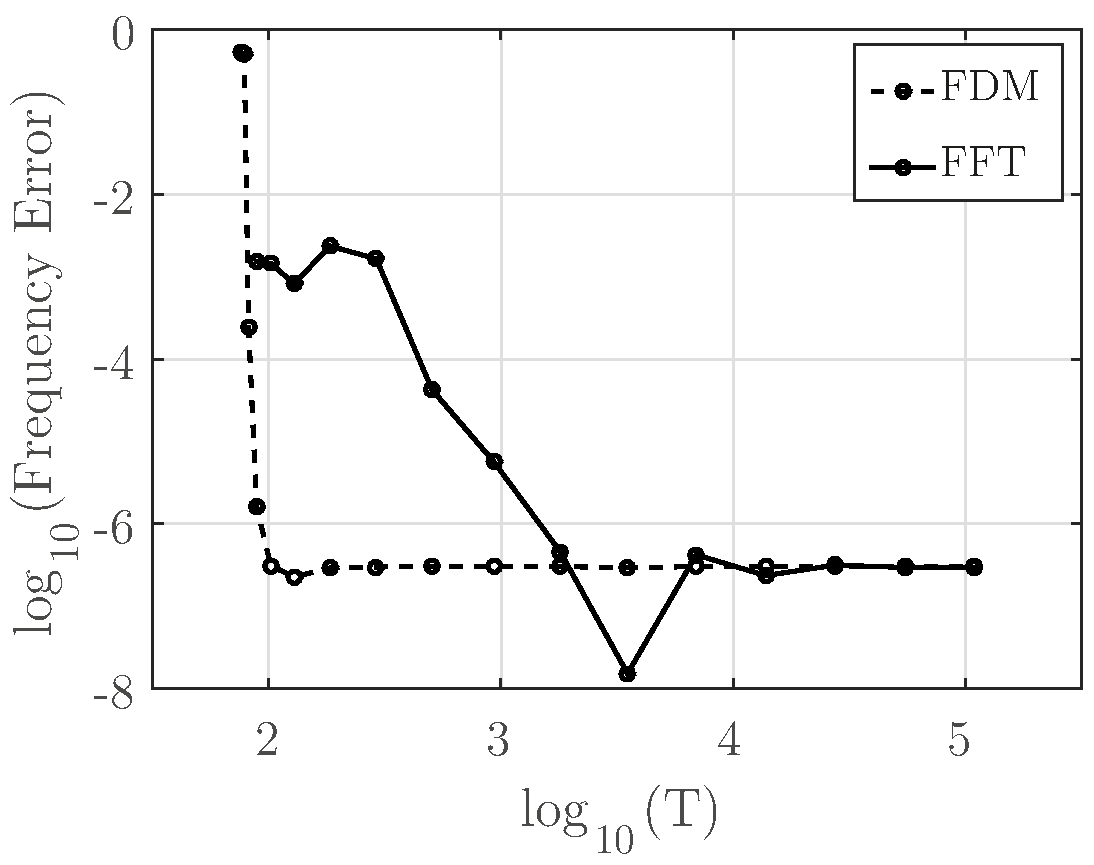
\includegraphics[width=0.6\textwidth]{figs/comparisonFFT_FDM}
	\caption{Error on a computed resonant frequency as a function of the length of the signal for FFT and FDM.}
	\label{fig:comparisonFFT_FDM}
\end{figure}
%TODO specify the units of time (T) somewhere in the text for an example
%geometry (so that I know what order they are for a problem of interest)
%text
It can be clearly observed that FDM is able to provide the same accuracy than FFT by reducing the final simulation time by more than two orders of magnitude. A detailed comparison of different frequency extraction techniques has been recently presented in~\cite{dantanarayana2014resonant}.

The choice of the monitor/s points can have an important effect on the final spectrum obtained. For instance, if a monitor point coincides (or it is very close) to a symmetry point of a particular mode, the frequency associated to this mode will not be obtained when applying the signal processing algorithm to the recorded signal. This effect has been studied in detail in~\cite{stark2009positional} and also can be utilised to avoid exciting undesired modes. 

Finally, it is worth mentioning that filters are commonly applied to the recorded fields to reduce the spectral leakage effect induced by the length of the signal~\cite{harris1978use,madisetti2009digital}. For the examples considered in this work the FDM is applied to the recorded signals and a Blackman filter is applied before extracting the frequency content. 

%=========================================================

\subsection{Resonant modes}
%text
\label{sc:modes}
After the resonant frequencies are computed, the associated resonant modes are computed by performing a second run of the time domain solver with a built-in discrete Fourier transform, namely
\begin{equation*}
    \hat{\USoltn}_j(f_k) = \sum_{n=0}^{\nT-1} \USoltn_j (t_n) \exp(-i2\pi t_n f_k), \quad j=1,\cdots,\nnode,
\end{equation*}
where $\nT$ is the total number of time steps, $\Delta t$ is the time step, $i = \sqrt{-1}$, $f_k$ are the computed resonant frequencies,  $t_n = n\Delta t$ and $\nnode$ is the total number of mesh nodes.


%=======================================================

\section{Numerical examples} 
%text
\label{sc:examples}

This sections presents a number of numerical examples to validate the implementation of the proposed technique for both free-space and dispersive materials. A comparison of the performance of low and high-order elements is presented and the effect of the geometric representation of cavities with curved boundaries on the accuracy and convergence properties of the proposed methodology are presented.

%============================================================

\subsection{Rectangular free space cavity}
%text
\label{sbc:freeSpace2D}

The first example involves the computation of the resonant frequencies and associated modes on a rectangular metallic cavity of dimension $2L \times L$ where $L=$20$\mu$m filled with air. The objective is to show the optimal convergence of the proposed approach for approximating the resonant frequencies and compare the performance of high and low-order approximations.  

The TM mode is considered and the frequencies are computed using a series of
structured quadrilateral meshes with 4$\times$2, 8$\times$4, 16$\times$8,
32$\times$16 and 64$\times$32 elements and different degrees of approximation.
The spectra obtained is shown in Figure~\ref{fig:rectangle2DfreeSpace_Spectrum}

EXAMPLE INTRODUCTION (PHYSICS)
\begin{itemize}
\item show the analytical solution
\item refer to a reference problem (i.e. length etc)
\item refer to a length of time for convergence in physical units
\item show a table of first 10 analytical solution values (up to $f=2$) with $f_1...f_10$ labels
\item include the analytical frequencies for the reference problem in the table
\end{itemize}
  
EXAMPLE INTRODUCTION (NUMERICS)
\begin{itemize}
\item initial condition, a point excitation, unity height at [0,0]
\item dt = 0.025 (as seen by FT, but not necessarily that of the simulation)
\item final time, $T = 2^(22) * 0.025$
\item specify the resolution in frequency space
\item hexagonal elements, uniform refinement
\item say that the way the initial condition is represented depends on the shape functions.
\item say that spectrum computed is the UNION of the amplitude all the components. motivation: shows all peaks detected)
\item note: TM only has one "good" component (which is U3), and TE has two U1 and U2 (but no U3) is the only component 
\end{itemize}
\begin{figure}[!ht]
	\centering
  \subfigure[4$\times$2, h-refinement]{
    \includegraphics[width=\textwidth]{2D_FreeSpaceCavity/SpectrumComparison/pVsH/hConv_2x4_legend}
    \label{fig:2D_FreeSpaceCavity:1x2_spectra_hConv}}
  \\
  \subfigure[4$\times$2, p-refinement]{
    \includegraphics[width=\textwidth]{2D_FreeSpaceCavity/SpectrumComparison/pVsH/pConv_2x4_legend}
    \label{fig:2D_FreeSpaceCavity:1x2_spectra_pConv}} \\
% /media/mark/slim/blueice_final/2D_FreeSpaceCavity_exampleSpectra/SpecComparisonPlot/original/allSameSourceAndMonitor/extraruns/signals
\end{figure}
Figure~\ref{fig:2D_FreeSpaceCavity:1x2_spectra_hConv}
\begin{itemize}
\item point out that the black line is the same on both
\item discuss the advantages of high order vs low order (higher frequency + higher amplitude)
\item Q:does the uniform length of time put $p=1$ at a disadvantage
\item say WHY we want higher amplitude...maybe this should have already happened by this stage?
\item all frequencies captured up to...
\item some comments about peak at zero
\end{itemize}

Figure~\ref{fig:2D_FreeSpaceCavity:1x2_spectra_pConv}
\begin{itemize}
\item Focus on the lowest frequency, compare the p=2 vs 8x16 coarse
  mesh, p=2 fne vs p=3 coarse (give ndof, nsteps for each example, total cpu time numbers)
\item compare number of degrees of freedom: href = 6    24    96, pref= 6 12 20
\item compare H2 + p=3 as having a similar number of degrees of freedom.
\item discuss the initial condition, we are using a delta function, which means that its representation in the mesh changes as we refine
\item mention that some frequencies are not captured
\item mention that this is due to initial condition, and could be modified by: gaussian, multiple initial conditions
\item show a plot of p=2, 16x8 with multiple initial conditions
\item need to mention peak WIDTH (for the same final time?), make sure the final time is ACTUALLY the same - width should be a measure of quality factor
\item mention that these are done using a Blackman envelope (haven't introduced this yet!!)
\item include a table with first 10 analytical frequencies
\end{itemize}

\begin{figure}[!ht]
	\centering
  \subfigure[8$\times$4, p-refinement]{
    \includegraphics[width=\textwidth]{2D_FreeSpaceCavity/SpectrumComparison/pVsH/pConv_4x8_legend}
    \label{fig:2D_FreeSpaceCavity:1x2_spectra_pConv}} \\
\end{figure}

Message: In practice, best results achieved with a combination of p and h refinement
Figure~\ref{fig:2D_FreeSpaceCavity:4x8_spectra_pConv}
\begin{itemize}
\item say a better resolution can be obtained from a combination of h and p refinement
\item conclude: mesh refinement improves ability to capture higher frequencies
\item for p=3 each peak in the range 0:2.5 corresponds exactly to a resonant frequency in the table above, i.e. the frequencies 1->33 are all captured. Above 2.5 some peaks are missing and badly captured.
\item compare ndof and amplitude/frequencies captured for each line with the href and pref
\end{itemize}

Message: Do not discard start of the signal...
TODO
Figure~\ref{fig:2D_FreeSpaceCavity:discardTimes_4x8_p3}
\begin{itemize}
\item discarding the initial signal has no effect (on signal)
\item Since signal duration is long, the effect on converged frequency estimate.
\item for the following examples the the 4x8, p=3 spectra is selected
\item message: don't discard the start
\item the effects of noise due to numerical dispersion (causing attenuation of the signal) seen.
\item higher frequencies attenuate more (due to low pass filtering of FEM)
\item the variation observed in the fundemental frequency between a discard time of 0 and 10000 is of the order $10^{13.5}$. (30 samples, uniformly distributed in log space).
\item Since signal duration is long, the effect on converged frequency estimate.
\end{itemize}

Message: start of signal is important...
TODO: no figure
\begin{itemize}
\item select the 4x8, p=3 spectra is selected
\item the effects of noise due to numerical dispersion (causing attenuation of the signal) seen.
\item higher frequencies attenuate more (due to low pass filtering of FEM)
\item the variation observed in the fundemental frequency between a discard time of 0 and 10000 is of the order $10^{13.5}$. (30 samples, uniformly distributed in log space).
\item Since signal duration is long, the effect on converged frequency estimate.
\end{itemize}

%============================================================
%============================================================

\clearpage
\subsection{Window functions}
%figure
\begin{figure}[!ht]
	\centering
  \subfigure[Rectangular]{\includegraphics[width=0.49\textwidth]{2D_FreeSpaceCavity/Windows/newRuns/filter_4x8_p3_Rect}}
  \subfigure[Gaussian]{\includegraphics[width=0.49\textwidth]{2D_FreeSpaceCavity/Windows/newRuns/filter_4x8_p3_Gaussian}}
  \subfigure[Blackman]{\includegraphics[width=0.49\textwidth]{2D_FreeSpaceCavity/Windows/newRuns/filter_4x8_p3_Blackman}}
  \subfigure[Blackman-Harris]{\includegraphics[width=0.49\textwidth]{2D_FreeSpaceCavity/Windows/newRuns/filter_4x8_p3_Blackman-Harris}}
\end{figure}
%figure DONE convergence with various windows
\begin{figure}[!ht]
	\centering
  \subfigure[$f_{3}$]{\includegraphics[width=0.45\textwidth]{2D_FreeSpaceCavity/Windows/conv/F3}} 
  \subfigure[$f_{4}$]{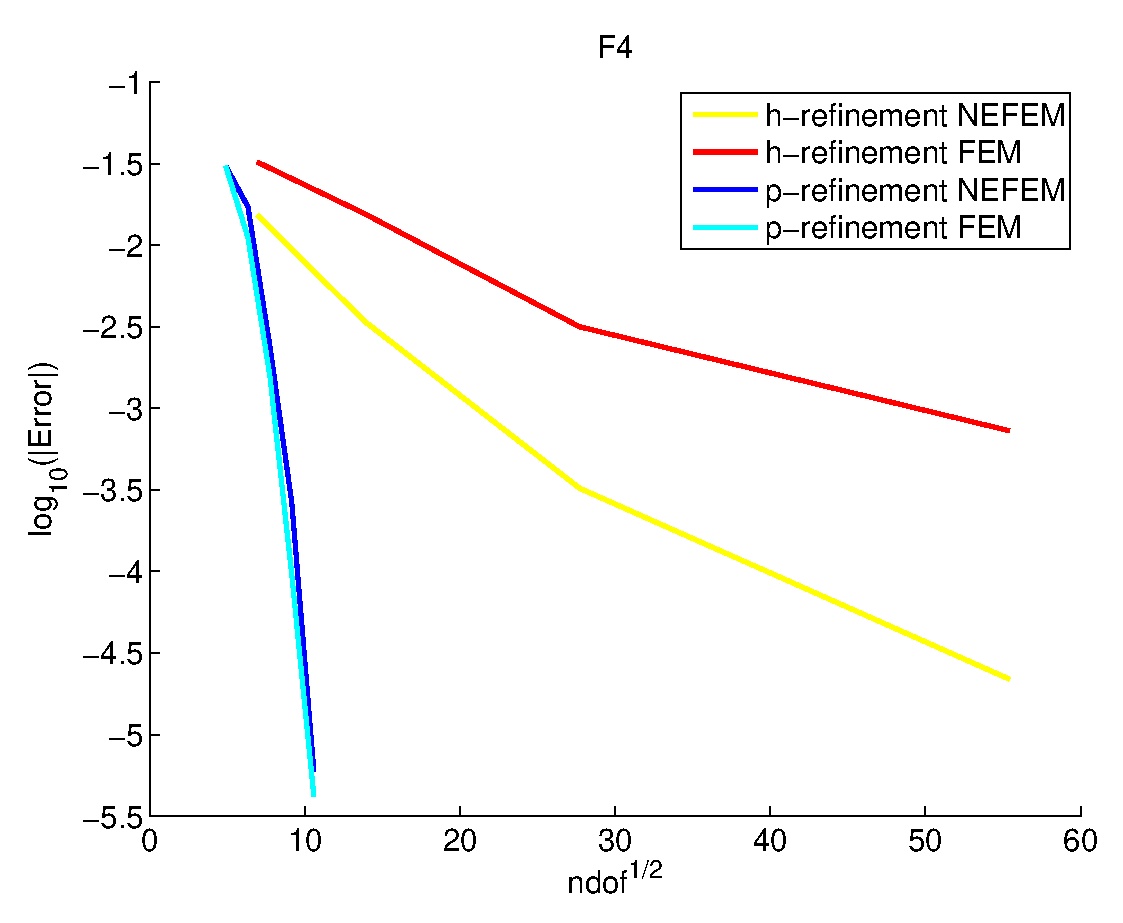
\includegraphics[width=0.45\textwidth]{2D_FreeSpaceCavity/Windows/conv/F4}}
  %\subfigure[$f_{8}$]{\includegraphics[width=0.45\textwidth]{2D_FreeSpaceCavity/Windows/conv/F8}}
  \subfigure[$f_{9}$]{\includegraphics[width=0.45\textwidth]{2D_FreeSpaceCavity/Windows/conv/F9}}
  \subfigure[$f_{10}$]{\includegraphics[width=0.45\textwidth]{2D_FreeSpaceCavity/Windows/conv/F10_legend}}
	\label{fig:rectangle2DfreeSpace_filteringConvergence}
\end{figure}

\begin{figure}[!ht]
	\centering
  \subfigure[Rectangular]{\includegraphics[width=\textwidth]{2D_FreeSpaceCavity/Windows/newRuns/filter_4x8_p3_Rect_spec}}
  \subfigure[Blackman]{\includegraphics[width=\textwidth]{2D_FreeSpaceCavity/Windows/newRuns/filter_4x8_p3_Blackman_spec}}
\end{figure}
for WINDOWS single-peak figures discuss:
NOTE: THE CONVERGENCE IN TIME PLOT IS DONE USING ZERO-PADDING (nothing else so far is)
\begin{itemize}
\item rectangular has minimal scalloping loss
\item rectangular has minimal scalloping loss
\item windows can be selected to sharpen peaks, but retain width
\item blackman, lots of loss of amplitude - but sharp peaks
\item blackman/blackman harris get there faster...Mention that the one Blackman perform better than the other for low frequencies and contrary for high frequencies so basically similar performance.
\item consistently perform better than rectangular window
\item Width of peaks
\item Noise
\item Discuss each one of them using the using the Fourier transform of the window itself. And basically conclude that you need to take a compromise. Refer to final time of 10000 (used here) and say that this is enough.
\end{itemize}

\clearpage
\subsection{Aliasing effects}
%figure
\begin{figure}[!ht]
	\centering
\subfigure[$\Delta t = 0.025$]{\includegraphics[width=\textwidth]{2D_FreeSpaceCavity/Aliasing/new/4x8_p3_dt=0_025}} \\
\subfigure[$\Delta t = 0.2$]{\includegraphics[width=\textwidth]{2D_FreeSpaceCavity/Aliasing/new/4x8_p3_dt=0_2}} \\
\subfigure[$\Delta t = 0.4$]{\includegraphics[width=\textwidth]{2D_FreeSpaceCavity/Aliasing/new/4x8_p3_dt=0_4}} \\
	\caption{Rectangular free-space cavity: spectrum with and without aliasing
    effects for two choices of timestep}
	\label{fig:rectangle2DfreeSpace_aliasing}
\end{figure}

Aliasing: Figure~\ref{fig:rectangle2DfreeSpace_aliasing}
Message: the time steps needs to be small enough
\begin{itemize}
\item T fixed at $2^{22}$ timesteps (as previous examples)
\item dt is increased
\item again, union of all components shown
\item no zero padding (yet)
\item additional peaks start appearing
\item location of peak not affected, but becomes harder to distinguish from noise
\end{itemize}

\begin{figure}[!ht]
	\centering
\includegraphics[width=\textwidth]{2D_FreeSpaceCavity/convergenceInTime/nTS2pow22_4x8_p3_f1_dt=0_025_legend} \label{fig:2D_FreeSpaceCavity:peakNarrowingInTime}
\end{figure}

Message: We need to run for long periods of time
Figure~\ref{fig:2D_FreeSpaceCavity:convergenceInTime}
TODO: need to adjust fonts on this figure...
\begin{itemize}
\item select the 4x8, p=3 spectra is selected (same dt)
\item refer up to figure on windows (showing convergence in time)
\item shown WITH window functions...
\item Figure~\ref{fig:2D_FreeSpaceCavity:peakNarrowingInTime} shows the narrowing of the peak with time
\item Figure~\ref{} shows the corresponding convergence of the frequency in time (rectangular window)
\item point out the time used in the previous examples, and the error associated with this time on the spectrum width/shape AND the final error (convergence in time)
\item high frequencies have higher error, due to the difficulty in capturing these frequencies, and the need for refinement.
\item low errors require a longer time
\end{itemize}

%figure TODO figure showing modes and convergence (i.e. FEM as a filter)

Message:zero padding can be used to improve resolution - but the spectra don't look the way one would expect
\begin{itemize}
\item started with previous in the first figure
\item done with RECTANGULAR window
\item other figures show zero padding in the close vicinity of the peak
\item frequency domain interpolation does not follow the way the untrained eye expects
\item amplitude loss (division by N)
\item iterpolation causes evidence of leakage to be visible - note this isn't CAUSED by zero padding, interpolation by zero padding interpolates the missing information missing?
\item note that lower resolution in the input signal, results in a lower resolution spectrum, regardless of zero padding
\item do I need to mention QFFT?
\end{itemize}

\begin{figure}[!ht]
	\centering
  \subfigure[$2^{22}$ timesteps without padding]{\includegraphics[width=0.45\textwidth]{2D_FreeSpaceCavity/zeroPadding/PAD_sig22_22}}
  \subfigure[$2^{19}$ timesteps, padded to $2^{22}$]{\includegraphics[width=0.45\textwidth]{2D_FreeSpaceCavity/zeroPadding/PAD_sig19_22}} \\
  % \subfigure[$2^{22}$ timesteps, padded to $2^{23}$]{\includegraphics[width=0.45\textwidth]{2D_FreeSpaceCavity/zeroPadding/PAD_sig22_23}}
  % \subfigure[$2^{19}$ timesteps, padded to $2^{23}$]{\includegraphics[width=0.45\textwidth]{2D_FreeSpaceCavity/zeroPadding/PAD_sig19_23}} \\
  % \subfigure[$2^{22}$ timesteps, padded to $2^{24}$]{\includegraphics[width=0.45\textwidth]{2D_FreeSpaceCavity/zeroPadding/PAD_sig22_24}}
  % \subfigure[$2^{19}$ timesteps, padded to $2^{24}$]{\includegraphics[width=0.45\textwidth]{2D_FreeSpaceCavity/zeroPadding/PAD_sig19_24}} \\
  \subfigure[$2^{22}$ timesteps, padded to $2^{25}$]{\includegraphics[width=0.45\textwidth]{2D_FreeSpaceCavity/zeroPadding/PAD_sig22_25}}
  \subfigure[$2^{19}$ timesteps, padded to $2^{25}$]{\includegraphics[width=0.45\textwidth]{2D_FreeSpaceCavity/zeroPadding/PAD_sig19_25}} \\
  \caption{Rectangular}
%
\end{figure}

\begin{figure}[!ht]
	\centering
  \subfigure[$2^{22}$ timesteps without padding]{\includegraphics[width=0.45\textwidth]{2D_FreeSpaceCavity/zeroPadding/PAD_Blackman_sig22_22}}
  \subfigure[$2^{19}$ timesteps, padded to $2^{22}$]{\includegraphics[width=0.45\textwidth]{2D_FreeSpaceCavity/zeroPadding/PAD_Blackman_sig19_22}} \\
  % \subfigure[$2^{22}$ timesteps, padded to $2^{23}$]{\includegraphics[width=0.45\textwidth]{2D_FreeSpaceCavity/zeroPadding/PAD_Blackman_sig22_23}}
  % \subfigure[$2^{19}$ timesteps, padded to $2^{23}$]{\includegraphics[width=0.45\textwidth]{2D_FreeSpaceCavity/zeroPadding/PAD_Blackman_sig19_23}} \\
  % \subfigure[$2^{22}$ timesteps, padded to $2^{24}$]{\includegraphics[width=0.45\textwidth]{2D_FreeSpaceCavity/zeroPadding/PAD_Blackman_sig22_24}}
  % \subfigure[$2^{19}$ timesteps, padded to $2^{24}$]{\includegraphics[width=0.45\textwidth]{2D_FreeSpaceCavity/zeroPadding/PAD_Blackman_sig19_24}} \\
  \subfigure[$2^{22}$ timesteps, padded to $2^{25}$]{\includegraphics[width=0.45\textwidth]{2D_FreeSpaceCavity/zeroPadding/PAD_Blackman_sig22_25}}
  \subfigure[$2^{19}$ timesteps, padded to $2^{25}$]{\includegraphics[width=0.45\textwidth]{2D_FreeSpaceCavity/zeroPadding/PAD_Blackman_sig19_25}} \\
	\label{fig:rectangle2DfreeSpace_filteringConvergence}
  \caption{Blackman}
\end{figure}

NOTE THE CHANGES IN SCALE

\begin{figure}[!ht]
	\centering
	\label{fig:rectangle2DfreeSpace_filteringConvergence}
\end{figure}
Figure~\ref{fig:rectangle2DfreeSpace_Convergence} shows the evolution of the
error on four computed resonant frequencies as a function of the element size
for a degree of approximation $p$ ranging from 1 up to 3. Each error is computed
from a single component. Figure (a) is computed from $E_2$, (b) from $E_1$, (c)
from $E_3$, (d) from $H_2$, and both (e) and (f) from $H_3$.
%figure
\begin{itemize}
\item TODO: cut out the points (p2 8x16) has some time marching error!
\item TODO: Add extra (higher error) points to make plots more asthetically
  pleasing
\item TODO: Add legends to all figures
\end{itemize}
\begin{figure}[!ht]
	\centering
   \subfigure[$f_{1} \approx, \USoltn_{2}, \TEz $]{\includegraphics[width=0.49\textwidth]{2D_FreeSpaceCavity/Conv/U[2]/F1_TE}}
   \subfigure[$f_{2} \approx, \USoltn_{1}, \TEz $]{\includegraphics[width=0.49\textwidth]{2D_FreeSpaceCavity/Conv/U[1]/F2_TE_legend}} \\
   \subfigure[$f_{3} \approx, \USoltn_{3}, \TMz $]{\includegraphics[width=0.49\textwidth]{2D_FreeSpaceCavity/Conv/U[3]/F3_TM_legend}}
   \subfigure[$f_{6} \approx, \USoltn_{2}, \TMz $]{\includegraphics[width=0.49\textwidth]{2D_FreeSpaceCavity/Conv/U[2]/F6_TM_legend}} \\
   \subfigure[$f_{8} \approx, \USoltn_{3}, \TMz $]{\includegraphics[width=0.49\textwidth]{2D_FreeSpaceCavity/Conv/U[3]/F8_TM_legend}}
   \subfigure[$f_{10} \approx, \USoltn_{3}, \TMz $]{\includegraphics[width=0.49\textwidth]{2D_FreeSpaceCavity/Conv/U[3]/F10_TM_legend}}
	\caption{Rectangular free-space cavity: $h$-convergence of the error for six resonant frequencies.}
	\label{fig:rectangle2DfreeSpace_Convergence}
\end{figure}
\begin{itemize}
\item RECTANGULAR CAVITY CONVERGENCE PLOTS
\item *only* a single component has been used, any component could have been used
\item refer to which components/modes used for which plot in the text
\item explain all components could have been used - this is easier
\item initial condition selected to excite these modes
\item find a reference for the 2p+2 convergence rate
\end{itemize}
%text
In this figure, and in subsequent examples, $f_i$ denotes the computed $i$-th resonant frequency and the frequencies are assumed ordered from lower to higher, i.e. $f_i < f_j$ if $i<j$. The error in the computed frequency $f_i$ is evaluated as $\epsilon_i = (|f_i - f_i^\star|)/f_i^\star$, where $f_i^\star$ is the known exact value of the resonant frequency~\cite{BalanisBook}.

In all the examples, the expected $2p+2$
%TODO - reference here for 2p+2 convergence rate...!
rate of convergence is approximately obtained, confirming the optimality of the proposed approach for computing the resonant frequencies of a free-space cavity. It can be observed that, for a given mesh and degree of approximation, the error increases as the frequency increases, illustrating the challenge in approximating higher frequencies. For instance, if the third mesh is used with a linear approximation (i.e., $p$=1), the resonant frequency $f_3 \approx$  8.38 THz is computed with an accuracy of $6.1 \times 10^{-4}$ whereas the error on the computed frequency $f_9 \approx$ 16.76 THz is $3.9 \times 10^{-3}$ (i.e. the error on the $f_9$ is more than 6 times higher than the error on the frequency $f_3$).

The results also illustrate the benefit of using high-order approximations. In the second mesh, the use of a cubic approximation of the solution offers a result almost four orders more accurate than using a linear approximation and two orders of magnitude more accurate than using a quadratic approximation. In the four cases presented in Figure~\ref{fig:rectangle2DfreeSpace_Convergence}, the use of a cubic approximation in the second mesh provides a similar accuracy than the computation in the finest mesh with a linear approximation. This implies that the computation with $p$=3 provides the same accuracy than the computation with $p$=1 by reducing the number of degrees of freedom by a factor of almost 20. It is worth mentioning that the required use of finer meshes with linear elements induces a significantly higher computational cost due to the use of an explicit time marching scheme.

After computing the resonant frequencies, the associated modes can be extracted by performing a discrete Fourier transform as described in Section~\ref{sc:FrequenciesAndModes}. Figure~\ref{fig:rectangle2DfreeSpace_modes} shows the second component of the electric field for the four modes associated to the frequencies $f_3$, $f_4$, $f_6$ and $f_9$.
%figure DONE Rectangular cavities
\begin{figure}[!ht]
	\centering
	\subfigure[$f_3 \approx$  8.38 THz]{\includegraphics[width=0.24\textwidth]{2D_FreeSpaceCavity/modeShapes/rectangleFreeSpace_U2_Mode2}}
	\subfigure[$f_4 \approx$ 10.60 THz]{\includegraphics[width=0.24\textwidth]{2D_FreeSpaceCavity/modeShapes/rectangleFreeSpace_U2_Mode3}}
	\subfigure[$f_6 \approx$ 13.51 THz]{\includegraphics[width=0.24\textwidth]{2D_FreeSpaceCavity/modeShapes/rectangleFreeSpace_U2_Mode5}}
	\subfigure[$f_9 \approx$ 16.76 THz]{\includegraphics[width=0.24\textwidth]{2D_FreeSpaceCavity/modeShapes/rectangleFreeSpace_U2_Mode6}} 
	\caption{Rectangular free-space cavity: component $E_2$ of four resonant modes.}
	\label{fig:rectangle2DfreeSpace_modes}
\end{figure}

%text
To further illustrate the potential of the proposed approach, Figure~\ref{fig:rectangle2DfreeSpace_modesHF} shows the first electric and magnetic component of the electromagnetic field corresponding to a high frequency mode, with associated resonant frequency of $f_{26} \approx 31.80$ THz. 
%figure DONE high-frequency rectangular cavities
\begin{figure}[!ht]
	\centering
	\subfigure[$E_1$]{\includegraphics[width=0.45\textwidth]{2D_FreeSpaceCavity/modeShapes/rectangleFreeSpace_2x4_p4_f15_U1}}
	\hspace{1cm}
	\subfigure[$H_1$]{\includegraphics[width=0.45\textwidth]{2D_FreeSpaceCavity/modeShapes/rectangleFreeSpace_2x4_p4_f15_U4}}
	\caption{Rectangular free-space cavity: two components of a high frequency resonant mode corresponding to the resonant frequency $f_{26} \approx 31.80$ THz.}
	\label{fig:rectangle2DfreeSpace_modesHF}
\end{figure}
%text
The computation has been performed on a very coarse mesh with only 8 elements and using a degree of approximation $p$=4 and the high quality of the mode shape can be clearly observed.

\clearpage
\subsection{Effect of the geometric representation for cavities with curved boundaries}
%text
The second example considers the computation of the resonant frequencies and associated modes in a metallic disk resonator of radius 1$\mu$m filled with air, for which an analytical solution is known~\cite{BalanisBook}. The objective is to study the effect of the geometric approximation of curved boundaries in the accuracy and convergence properties of isoparametric finite elements and NEFEM. In addition, the benefits of using high-order curved elements in this context are quantified using the computational time. 

The resonator is discretised using a series of unstructured triangular meshes with 4, 16, 64, 256, and 1,024 elements and with different orders of approximation. Figure~\ref{fig:circleFEMvsNEFEM_Convergence} (a) shows the evolution of the error in the first resonant frequency, $f_1 \approx$ 57.59 THz, as a function of the element size for linear and quadratic elements and by using standard isoparametric finite elements and NEFEM. 
%figure REVISE - 2D Circle convergence comparison - more of them!
\begin{figure}[!ht]
	\centering
	\subfigure[$h$-refinement]{\includegraphics[width=0.49\textwidth]{2D_Circle/convergenceFigures/circleFreeSpce_hRef_legend}}
	\subfigure[$p$-refinement]{\includegraphics[width=0.49\textwidth]{2D_Circle/convergenceFigures/circleFreeSpce_pRef_legend}}
	\caption{Disk resonator: $h$-convergence and $p$-convergence of the error for the first resonant frequency $f_1$.}
	\label{fig:circleFEMvsNEFEM_Convergence}
\end{figure}
%text
The results show that the geometric approximation of curved boundaries introduced by standard finite elements induce not only a significant loss of accuracy but, more importantly, a loss of the optimal rate of convergence. For example, in the fourth mesh, with 256 elements and using a linear approximation of the solution, the error on the resonant frequency with NEFEM is more than two orders of magnitude lower than the error obtained by using standard finite elements. For isoparametric finite element a rate of convergence $2p$ is observed whereas for NEFEM the optimal rate of convergence, $2p+2$, is observed. 

Figure~\ref{fig:circleFEMvsNEFEM_Convergence} (b) shows a $p$-refinement study. The first mesh, with only four elements, is considered and the degree of approximation is increased from $p$=1 to $p$=4. The evolution of the error in the first resonant frequency as a function of the square root of the number of degrees of freedom is shown for isoparametric finite elements and NEFEM. The comparison shows important differences for low order approximations (i.e, $p$=1,2) whereas for higher order approximations (i.e, $p \geq$3), a similar error is obtained suggesting that a high order approximation of the geometry is mandatory is order to avoid an effect on the computed resonant frequencies. 

Figure~\ref{fig:circle2DfreeSpace_modes} shows the third component of the electric field for twelve modes. 
%figure DONE Circle Mode Shapes
\begin{figure}[!ht]
\centering
\subfigure[$f_1 \approx$ 57.37 THz]{\includegraphics[width=0.24\textwidth] {2D_Circle/modeShapes/circleFreeSpace_mode1_U3}}
\subfigure[$f_2 \approx$ 91.41 THz]{\includegraphics[width=0.24\textwidth] {2D_Circle/modeShapes/circleFreeSpace_mode2_U3}}
\subfigure[$f_3 \approx$ 122.52 THz]{\includegraphics[width=0.24\textwidth] {2D_Circle/modeShapes/circleFreeSpace_mode3_U3}}
\subfigure[$f_{14} \approx$ 263.97 THz]{\includegraphics[width=0.24\textwidth] {2D_Circle/modeShapes/circleFreeSpace_mode14_U3}} \\
%
\subfigure[$f_4 \approx$ 131.69 THz]{\includegraphics[width=0.24\textwidth] {2D_Circle/modeShapes/circleFreeSpace_mode4_U3}}
\subfigure[$f_6 \approx$ 167.37 THz]{\includegraphics[width=0.24\textwidth] {2D_Circle/modeShapes/circleFreeSpace_mode6_U3}}
\subfigure[$f_5 \approx$ 152.21 THz]{\includegraphics[width=0.24\textwidth] {2D_Circle/modeShapes/circleFreeSpace_mode5_U3}}
\subfigure[$f_{19} \approx$ 294.36 THz]{\includegraphics[width=0.24\textwidth] {2D_Circle/modeShapes/circleFreeSpace_mode19_U3}} \\
%
\subfigure[$f_{17} \approx$ 281.31 THz]{\includegraphics[width=0.24\textwidth] {2D_Circle/modeShapes/circleFreeSpace_mode17_U3}}
\subfigure[$f_{13} \approx$ 242.71 THz]{\includegraphics[width=0.24\textwidth] {2D_Circle/modeShapes/circleFreeSpace_mode13_U3}}
\subfigure[$f_7 \approx$ 181.03 THz]{\includegraphics[width=0.24\textwidth] {2D_Circle/modeShapes/circleFreeSpace_mode7_U3}}
\subfigure[$f_{20} \approx$ 310.50 THz]{\includegraphics[width=0.24\textwidth] {2D_Circle/modeShapes/circleFreeSpace_mode20_U3}} 
\caption{Disk resonator: component $H_3$ of twelve resonant modes.}
\label{fig:circle2DfreeSpace_modes}
\end{figure}
%text
These modes are extracted by performing a discrete Fourier transform as described in Section~\ref{sc:FrequenciesAndModes}. All the modes were computed using a single time domain run on a mesh with 
only 1,024 elements and using a degree of approximation $p$=5 (i.e, 46,080 degrees of freedom) and the error on the highest computed resonant frequency ($f_{20} \approx$ 310.50 THz) is less than 0.3\%. This clearly illustrate the potential of the proposed approach for computing a broadband of resonant frequencies and the associated modes using NEFEM with a DG formulation in the time domain.

Next, the performance of both low and high-order approximations is studied. Figure~\ref{fig:circleHvsP} shows the evolution of the error of the first computed resonant frequency as a function of the number of degrees of freedom (\ndof) and the CPU time for low and high-order approximations. In both cases NEFEM is considered in order to avoid any error introduced by the polynomial approximation of curved boundaries inherent to standard isoparametric finite elements.
%figure REVISE : Circle convergence CPU times
\begin{figure}[!ht]
	\centering
  \subfigure[degrees of freedom]{\includegraphics[width=0.49\textwidth]{2D_Circle/convergenceFigures/circleFreeSpce_ndof_legend}}
  \subfigure[Wall time]{\includegraphics[width=0.49\textwidth]{2D_Circle/convergenceFigures/circleFreeSpce_cpu_legend}}
	\caption{Disk resonator: Comparison of $h$ and $p$ refinement in terms of (a) the number of degrees of freedom (\ndof) and (b) the wall time for the computation of the first resonant frequency $f_1$.}
	\label{fig:circleHvsP}
\end{figure}
%text
The comparison in terms of number of degrees of freedom in Figure~\ref{fig:circleHvsP} (a) shows, as expected that high-order elements significantly outperform low-order elements when the solution is smooth due to the exponential rate of convergence of a $p$-refinement strategy compared to the algebraic rate of an $h$-refinement strategy. In this example, for an error in the first resonant frequency of $10^{-4}$ the number of degrees of freedom required using NEFEM with linear approximation is 1,149, whereas the same accuracy can be obtained using approximately 204 degrees of freedom. For high accurate results, namely an error in the first resonant frequency of $2.5 \times 10^{-7}$, the use of high-order methods is even more advantageous. NEFEM with linear approximation requires 18,432 degrees of freedom, whereas the same accuracy can be obtained using only 360 degrees of freedom. 

The save in number of degrees of freedom introduced by a high-order functional approximation has been consistently observed in many examples and it is probably a crucial factor for the growing interest in high-order methods not only by the computational electromagnetics and but also by the computational fluid dynamics community~\cite{ADIGMA,HO-Fluids}. In some examples this save is not translated in a lower computational cost due to the extra computational cost per element induced by a high-order approximation. Figure~\ref{fig:circleHvsP} (b) shows the comparison of low and high-order approximations in terms of the normalised CPU time (i.e, dividing by the computational cost of linear elements in the coarse mesh) in logarithmic scale. The results demonstrate that high-order methods are not only competitive in terms of memory requirements, but more importantly, in terms of the computing time. In this example, an error in the first resonant frequency of $10^{-4}$ can be achieved using high-order elements 5.5 times faster than using linear elements. For high accurate results, namely an error in the first resonant frequency of $2.5 \times 10^{-7}$, high-order elements are 88 times faster than linear elements.

It is worth noting that the speed up factor of high-order elements compared to low-order elements is similar, or even higher, than the factor by which the number of degrees of freedom is reduced, clearly illustrating the potential and performance of high-order elements for the computation of resonant frequencies in cavities.


%============================================================
\clearpage
\subsection{Effect of the monitor position choice for cavities}
\clearpage
%figure TODO : Plots for effects of monitor positions - take them from ACME and change unit system as appropriate
\subsection{Rectangular dispersive cavity}
%text
The next example considers a rectangular cavity of dimension $2L \times L$, with $L=$20$\mu$m made of a dispersive material with non-dimensional constants $\omega_p = 0.7933$ and $\gamma = 0.076$ and with a perfect electric conducting boundary.

First, the implementation of the DG method for a lossless single-pole Drude media with no magnetic polarisation is validated by considering the propagation of a mode in the cavity. A volumetric source term is considered so that the analytical solution is
% 
\begin{equation*}
\E = \sin (\pi t) 
\begin{pmatrix}
- \cos (\pi x_1) \sin (\pi x_2) \\
  \sin (\pi x_1) \cos (\pi x_2) \\
2 \sin (\pi x_1) \sin (\pi x_2) 
\end{pmatrix}
%
\quad
%
\H = \cos (\pi t) 
\begin{pmatrix}
- \sin (\pi x_1) \cos (\pi x_2) \\
  \cos (\pi x_1) \sin (\pi x_2) \\
- \cos (\pi x_1) \cos (\pi x_2) 
\end{pmatrix}.
\end{equation*}

The computations are performed on a series of uniformly refined unstructured triangular meshes with elements and for a degree of approximation from $p$=1 to $p$=4. Initial and boundary conditions corresponding to the analytical solution are considered.

\begin{figure}[!ht]
	\centering
	\subfigure[$E_1$]{\includegraphics[width=0.49\textwidth]{2D_DispersiveVolumetricSource/soltnT3_TRI_H4_p2_E1}}
	\subfigure[$E_2$]{\includegraphics[width=0.49\textwidth]{2D_DispersiveVolumetricSource/soltnT3_TRI_H4_p2_E2}}
	\subfigure[$E_3$]{\includegraphics[width=0.49\textwidth]{2D_DispersiveVolumetricSource/soltnT3_TRI_H4_p2_E3}}
	\caption{Rectangular dispersive cavity: snapshots of the electric field intensity obtained from a 136 element mesh with $p=2$ at $T=3$.}
	\label{fig:rectangle2DdispersiveTest_Convergence}
\end{figure}

Figure~\ref{fig:rectangle2DdispersiveTest_Convergence} shows the $\mathcal{L}^2(\Omega)$ norm of the error of two components of the electromagnetic field, namely $E_1$ and $H_3$, as a function of the characteristic element size $h$. In all cases, the expected optimal rate of convergence (i.e, $p$+1) is observed. 
%figure DONE: Volumetric source convergence
\begin{figure}[!ht]
	\centering
	\subfigure[$E_1$]{\includegraphics[width=0.49\textwidth]{figs/dispersiveHconv_U1}}
	\subfigure[$H_3$]{\includegraphics[width=0.49\textwidth]{figs/dispersiveHconv_U3}}
	\caption{Rectangular dispersive cavity: $h$-convergence of the $\mathcal{L}^2(\Omega)$ norm of the error of two components of the electromagnetic field as a function of the characteristic element size $h$ for different degrees of approximation ($p$).}
	\label{fig:rectangle2DdispersiveTest_Convergence}
\end{figure}
%text
Next, the convergence properties of the proposed technique for the computation of resonant frequencies in a dispersive cavity are validated. As no analytical solution is available for the resonant frequencies, a reference solution is computed using a mesh with 2048 elements and a degree of approximation $p$=3.  The error in the computed frequency $f_i$ is evaluated as $\epsilon_i = (|f_i - f_i^r|)/f_i^r$, where $f_i^r$ is the reference value of the resonant frequency.

Figure~\ref{fig:rectangle2Ddispersive_Convergence} shows the evolution of the error on two computed resonant frequencies as a function of the element size for linear and quadratic elements. 
%figure DONE: dispersive convergence
\begin{figure}[!ht]
	\centering

\subfigure[$f_{3},\USoltn_{3} $]{\includegraphics[width=0.49\textwidth]{2D_DispersivePlate/Conv/F3_U3_TM}}
\subfigure[$f_{6},\USoltn_{3} $]{\includegraphics[width=0.49\textwidth]{2D_DispersivePlate/Conv/F6_U3_TM}}
\subfigure[$f_{8},\USoltn_{3} $]{\includegraphics[width=0.49\textwidth]{2D_DispersivePlate/Conv/F8_U3_TM}}
\subfigure[$f_{9},\USoltn_{2} $]{\includegraphics[width=0.49\textwidth]{2D_DispersivePlate/Conv/F9_U2_TM}}
\subfigure[$f_{10},\USoltn_{3} $]{\includegraphics[width=0.49\textwidth]{2D_DispersivePlate/Conv/F10_U3_TM} }
	\caption{Rectangular dispersive cavity: $h$-convergence of the error for two resonant frequencies.}
	\label{fig:rectangle2Ddispersive_Convergence}
\end{figure}
%text
In all the examples, the expected $2p+2$ rate of convergence is approximately obtained, confirming the optimality of the proposed approach for computing the resonant frequencies of cavities filled with dispersive materials. As in previous examples, it can be observed that, for a given mesh and degree of approximation, the error increases as the frequency increases, illustrating the challenge in approximating higher frequencies. 


The effect of the dispersive material in the signal recorded at a point of the cavity is shown in Figure~\ref{fig:freeSpaceDispersiveSignal} by comparing the results to the ones obtained in the free-space cavity discussed in Section~\ref{sbc:freeSpace2D}.
%figure DONE: dispersive signal(unfiltered)
\begin{figure}[!ht]
	\centering
	\subfigure[]{\includegraphics[width=0.49\textwidth]{figs/freeSpaceDispersiveSignal1}}
	\subfigure[]{\includegraphics[width=0.49\textwidth]{figs/freeSpaceDispersiveSignal2}}
	\caption{Rectangular dispersive cavity: Comparison of the time recorded signal corresponding to the component $H_3$ at a point of the cavity for free-space and dispersive media.}
	\label{fig:freeSpaceDispersiveSignal}
\end{figure}
%text
It can be observed in Figure~\ref{fig:freeSpaceDispersiveSignal}(a) that in initially the signals are very similar in shape and phase despite important differences are already observed in the amplitude. As represented in Figure~\ref{fig:freeSpaceDispersiveSignal}(b) for latter times the recorded signals vary significantly.

Finally, Figure~\ref{fig:dispersiveFreeSpaceSpectrum} shows the computed spectrum for both the free-space cavity and the dispersive cavity using, in both cases, a mesh with 128 elements and a degree of approximation $p$=2. 
%figure LATER: dispersive spectrum comparison -  can I do better?
\begin{figure}[!ht]
\centering
\includegraphics[width=\textwidth]{2D_DispersivePlate/SpectrumComparison/dispVsNonDisp}
\caption{Rectangular dispersive cavity: Comparison of computed spectra for a for free-space and dispersive cavity.}
\label{fig:dispersiveFreeSpaceSpectrum}
\end{figure}

\begin{figure}[!ht]
\centering
\subfigure[$f_1,E_3$]{\includegraphics[width=0.46\textwidth]{2D_DispersivePlate/Modes/F1_U3}}
\subfigure[$f_2,H_1$]{\includegraphics[width=0.46\textwidth]{2D_DispersivePlate/Modes/F2_U1}}
\subfigure[$f_2,H_2$]{\includegraphics[width=0.46\textwidth]{2D_DispersivePlate/Modes/F2_U2}}
\subfigure[$f_2,E_3$]{\includegraphics[width=0.46\textwidth]{2D_DispersivePlate/Modes/F2_U3}}
\subfigure[$f_3,H_2$]{\includegraphics[width=0.46\textwidth]{2D_DispersivePlate/Modes/F3_U2}}
\subfigure[$f_5,H_2$]{\includegraphics[width=0.46\textwidth]{2D_DispersivePlate/Modes/F5_U2}}
\subfigure[$f_6,E_3$]{\includegraphics[width=0.46\textwidth]{2D_DispersivePlate/Modes/F6_U3}}
\caption{Rectangular dispersive cavity: mode shapes for a 32 element mesh, with $p=2$.}
\label{fig:dispersiveFreeSpaceSpectrum}
\end{figure}

\begin{figure}[!ht]
\centering
\subfigure[$f_5,|\mathbf{H}|$]{\includegraphics[width=0.46\textwidth]{2D_DispersivePlate/Modes/F5_AmpH}}
\caption{Rectangular dispersive cavity: mode shapes for a 32 element mesh, with $p=2$.}
\label{fig:dispersiveFreeSpaceSpectrum}
\end{figure}

frequencies:
0.573093071579933
0.718288226075311
0.910187134866009
1.038485020399094
1.125144932732563
1.256364956498146
1.352221811226707
1.419845223426819
1.526010036468506
1.586255573838266
1.605777069926262
1.681876927614212
1.807270944118500
1.824646443128586
1.956731081008911

/Data/2D_DispersiveCavity/modeShapes/nOfCyclesMax_500
%text
The results reveal a shift of all the frequencies, being more important for low frequencies than for the higher frequencies. It can also be observed that the amplitude is lower for the dispersive cavity compared to the cavity filled with air.


%============================================================
\clearpage
\subsection{Three dimensional cavities with planar faces}
%text
The next example considers a three dimensional metallic cavity of dimension $L\times L \times L$, where $L$=2$\mu$m filled with air, for which an analytical solution is known~\cite{BalanisBook}. The objective is to validate the implementation and illustrate the potential of the proposed approach in three dimensions.  

The frequencies are computed using a series of structured hexahedral meshes with 2$\times$2$\times$2, 4$\times$4$\times$4, 8$\times$8$\times$8 and 16$\times$16$\times$16 elements and different degrees of approximation. Although the use of tetrahedral meshes is preferred for geometrically complex cavities, the use of hexahedral elements, when possible, reduces significantly the cost of the time domain solver due to the reduced number of interior faces compared to a tetrahedral mesh. The performance of different elements was studied in detail in~\cite{HybridMeshesCEM} and it was concluded that in order to obtain the same accuracy hexahedral elements require between 10 to 15 less computational time than tetrahedral elements.

The evolution of the error on two computed resonant frequencies as a function of the element size for a degree of approximation $p$ ranging from 1 up to 3 is shown in Figure~\ref{fig:cube3DfreeSpace_ConvergenceTet} for tetrahedral elements and in Figure~\ref{fig:cube3DfreeSpace_ConvergenceHex} for hexahedral elements.

\begin{figure}[!ht]
	\centering
	\subfigure[$f_5    \approx$ 1.118, $\USoltn_{1}$]{\includegraphics[width=0.49\textwidth]{3D_CubeCavity/Conv/HEX/U[1]/F5_CF}}
	\subfigure[$f_6    \approx$ 1.225, $\USoltn_{6}$]{\includegraphics[width=0.49\textwidth]{3D_CubeCavity/Conv/HEX/U[6]/F6_CF}}
	\subfigure[$f_9    \approx$ 1.581, $\USoltn_{4}$]{\includegraphics[width=0.49\textwidth]{3D_CubeCavity/Conv/HEX/U[4]/F9_CF}}
	\subfigure[$f_{10} \approx$ 1.658, $\USoltn_{2}$]{\includegraphics[width=0.49\textwidth]{3D_CubeCavity/Conv/HEX/U[2]/F10_CF}}

	\caption{Three dimensional cavity: $h$-convergence of the error for a selection of four choices of resonant frequency and solution component using hexahedral elements.}
	\label{fig:cube3DfreeSpace_ConvergenceHex}
\end{figure}
%viva - higher frequencies more challenging in 3D
%text
The results demonstrate the optimal convergence properties of the proposed approach to compute the resonant frequencies in three dimensional cavities and illustrate the challenge of computing high resonant frequencies as the accuracy of the frequency $f_5$ is almost two orders of magnitude higher than the accuracy for the frequency $f_9$. 

In addition, it is important to remark that the save in terms of number of degrees of freedom is more significant here than for the two dimensional problems discussed before. For instance, in order to obtain a relative error on the frequency $f_9$ below $10^{-4}$, cubic elements employ a mesh with 64 elements (i.e, 1,280 degrees of freedom), quadratic elements require a mesh with 512 elements (i.e, 5,120 degrees of freedom) and linear elements require a further level of mesh refinement (not considered in Figure~\ref{fig:cube3DfreeSpace_Convergence}(b)), resulting in a mesh with 32,768 elements (i.e, 131,072 degrees of freedom). This means that cubic elements are able to perform a similar accuracy compared to linear elements by reducing the number of degrees of freedom by more than two orders of magnitude.

The resonant modes are again computed using another time domain simulation as described in Section~\ref{sc:FrequenciesAndModes}. Figure~\ref{fig:cubeFreeSpace_1stMode} shows the three components of the electric field for the resonant mode associated to the lowest frequency, $f_1 \approx$ 105.99 THz.
%figure DONE: 3D Cube mode shapes different components
\begin{figure}[!ht]
	\centering
	\subfigure[$E_1$]{\includegraphics[width=0.32\textwidth] {3D_CubeCavity/modeShapes/Cube_Mode2_U1}}
	\subfigure[$E_2$]{\includegraphics[width=0.32\textwidth] {3D_CubeCavity/modeShapes/Cube_Mode2_U2}}
	\subfigure[$E_3$]{\includegraphics[width=0.32\textwidth] {3D_CubeCavity/modeShapes/Cube_Mode2_U3}}
	\caption{Three dimensional cavity: three components of the electric field for the first resonant mode with frequency $f_1 \approx$ 105.99 THz.}
	\label{fig:cubeFreeSpace_1stMode}
\end{figure}

%text
To further illustrate the potential of the proposed methodology, Figure~\ref{fig:cubeFreeSpace_modes} shows the intensity of the electric and magnetic fields for four resonant modes, associated to the resonant frequencies $f_4\approx$ 167.59 THz, $f_6\!\approx$ 211.99 THz, $f_{35} \approx$ 491.47 THz and $f_{36} \approx$ 502.77 THz.
%figure TODO: better 3D Cube mode shapes
\begin{figure}[!ht]
	\centering
	\subfigure[$\!\!\!E, f_4\!\approx$167.6 THz]{\includegraphics[width=0.24\textwidth]{3D_CubeCavity/modeShapes/Cube_Mode5_E}}
	\subfigure[$\!\!\!E, f_6\!\approx$212.0 THz]{\includegraphics[width=0.24\textwidth]{3D_CubeCavity/modeShapes/Cube_Mode7_E}}
	\subfigure[$\!\!\!E, f_{35}\!\approx$491.5 THz]{\includegraphics[width=0.24\textwidth]{3D_CubeCavity/modeShapes/Cube_Mode36_E}}
	\subfigure[$\!\!\!E, f_{36}\!\approx$502.8 THz]{\includegraphics[width=0.24\textwidth]{3D_CubeCavity/modeShapes/Cube_Mode37_E}} \\
	\subfigure[$\!\!\!H, f_4\!\approx$167.6 THz]{\includegraphics[width=0.24\textwidth]{3D_CubeCavity/modeShapes/Cube_Mode5_H}}
	\subfigure[$\!\!\!H, f_6\!\approx$212.0 THz]{\includegraphics[width=0.24\textwidth]{3D_CubeCavity/modeShapes/Cube_Mode7_H}}
	\subfigure[$\!\!\!H, f_{35}\!\approx$491.5 THz]{\includegraphics[width=0.24\textwidth]{3D_CubeCavity/modeShapes/Cube_Mode36_H}}
	\subfigure[$\!\!\!H, f_{36}\!\approx$502.8 THz]{\includegraphics[width=0.24\textwidth]{3D_CubeCavity/modeShapes/Cube_Mode37_H}} 
	\caption{Three dimensional cavity: intensity of the electric (top) and magnetic (bottom) fields for four resonant modes.}
	\label{fig:cubeFreeSpace_modes}
\end{figure}

%text
All the modes have been computed on a mesh with only 64 hexahedral elements and using a degree of approximation $p=3$ (i.e, 7,680 degrees of freedom) and the relative error in the four resonant frequencies associated to the mode represented in Figure~\ref{fig:cubeFreeSpace_modes}, ranging from 167.59 THz to 502.77 THz is below $10^{-5}$.

\clearpage
\subsection{Three dimensional cavities with curved faces}
%text TODO introduce 3D Sphere
%figures TODO show some figures of 3D Sphere

\clearpage
\subsection{Cavities with small features}
Meshes
- Discuss the required mesh refinement with FEM and how this can be avoided with NEFEM. (provide number of elements and induced time step).
Show figures.
\begin{itemize}
\item Show the spectrum with a scale such that the two peaks are hardly differentiated (or not at all). Include a box explaining that this will be zoomed in.
\item Show the modes
\item Qualitative comparison with the dielectric circle.
\item This will be the first problem with multi-material.
\item You can show here results of the dielectric circle 
\item You can show two different materials to show different frequencies where the split happens.
\end{itemize}

%figure
\begin{figure}[!ht]
	\centering
\subfigure[without scatterers]{\includegraphics[width=0.49\textwidth]{NotchedAndSpiral/peakCircleOnly}}
\subfigure[with scatterers]{\includegraphics[width=0.49\textwidth]{NotchedAndSpiral/peakNotchOnly}}
\subfigure[with and without scatterers]{\includegraphics[width=0.49\textwidth]{NotchedAndSpiral/peakNotchAndCircle}}
	\caption{Rectangular dispersive cavity: $h$-convergence of the error for two resonant frequencies.}
	\label{fig:rectangle2Ddispersive_Convergence}
\end{figure}
%text TODO introduce 3D Sphere
\section{Parallel}
\subsection{3D Convergence plots}
single p strong scaling plot
\begin{itemize}
\item use these plots to justify that communication it not relevant, so the most important is to distribute the work among all the processor properly ---> not sure about this statement, but I need a conclusion
\item You could add two different communication strategies.
\item do I need another figure with bigger meshes.
\item This figure shows that when all the elements have the same p you just need to the same number of elements per processor, so the only thing is to minimise  interfaces in between processors (parametis)
\end{itemize}
\begin{figure}[!ht]
	\centering
  \includegraphics[width=0.49\textwidth]{Parallel/3DSpeedPlot_unitCube_legend}
	\caption{3D unit cube: timings obtained with a non-uniform mesh}
	\label{fig:unitCubeNonUniformTimings}
\end{figure}
\clearpage
\subsection{3D Non-Uniform Cube}
DESCRIPTION OF MESH:
\begin{itemize}
\item SHOW THE MESH and explaining the rationale of the test.
Show a table with rows showing p=1,...,9.
Columns showing min nwl and max nwl. THis motivates variable p.
\item: TO THINK ABOUT. Including delta t. This will need s study of the stability limit for different p.
  %http://wwwhome.math.utwente.nl/~botchevma/sarmany_ea07.pdf
\item In many applications the mesh is generated so that a uniform distribution of nodes per wavelength are obtained. In the presence of small features you propose to use variable p to alleviate the meshing constraint.
\item Provide in the text the min and max element size, time step induced if you were to use 
\end{itemize}
%TODO FIGURE - show the mesh and partition

\begin{figure}[!ht]
	\centering
  \subfigure[histogram]{\includegraphics[width=0.49\textwidth]{Parallel/3D_UnitCube_nonUniform/elementSizeHsitogram}}
  \subfigure[histogram]{\includegraphics[width=0.49\textwidth]{Parallel/3D_UnitCube_nonUniform/pHistogram}}
\caption{3D unit cube: histograms of p and element size}
	\label{fig:unitCubeNonUniformTimings}
\end{figure}

speed(normalised): 0.5551    0.6592    1.0000
(computed from minimum timestep length)
\begin{figure}[!ht]
	\centering
  \subfigure[unweighted]{\includegraphics[width=0.49\textwidth]{Parallel/3D_UnitCube_nonUniform/noWeighting}} \\
  \subfigure[by measurement]{\includegraphics[width=0.49\textwidth]{Parallel/3D_UnitCube_nonUniform/computedWeighting}}
  \subfigure[by operation count]{\includegraphics[width=0.49\textwidth]{Parallel/3D_UnitCube_nonUniform/analyticalWeighting}}
	\caption{3D unit cube: timings obtained with a non-uniform mesh}
	\label{fig:unitCubeNonUniformTimings}
\end{figure}

16689 elements
3437 nodes
Tets
\begin{figure}[!ht]
	\centering
\subfigure[]{\includegraphics[width=0.49\textwidth]{Parallel/3D_UnitCube_nonUniform/weightingComparison_legend}}
\caption{3D unit cube: weighting comparison}
	\label{fig:unitCubeNonUniformTimings}
\end{figure}
change in delta t is only 6x
hMin=0.003963734230961


\section{Variable order}
%figure done 3D Cube Exploded
\begin{figure}[!ht]
	\centering
  \includegraphics[width=\textwidth]{3D_SphereExploded/sphereDots}
	\caption{3D unit cube: timings obtained with a non-uniform mesh}
	\label{fig:unitCubeNonUniformAdaptiveP}
\end{figure}
\begin{figure}[!ht]
	\centering
\includegraphics[width=\textwidth]{Parallel/globalL2Convergence}
\caption{3D unit cube: global convergence of L2 norm of the solution}
	\label{fig:unitCubeNonUniformGlobalAdaptivePL2Conv}
\end{figure}
L2 computed at $T=1$
% text TODO
%% * use the same dimensions as the 3D Cube
\section{Photonic Crystals}
\begin{figure}[!ht]
	\centering
  \includegraphics[width=0.49\textwidth]{PhC/PhCHexagonal}
\end{figure}
NEFEM mesh
TODO: mesh details (number of elements etc)
\begin{figure}[!ht]
	\centering
\subfigure[$f_{2}, \USoltn_{3}$]{\includegraphics[width=0.49\textwidth]{PhC/modeShapes/frame2_U3_nurbsZoom}}
\subfigure[$f_{5}, \USoltn_{2}$]{\includegraphics[width=0.49\textwidth]{PhC/modeShapes/frame5_U2_nurbsZoom}}
\subfigure[$f_{4}, \USoltn_{2}$]{\includegraphics[width=0.49\textwidth]{PhC/modeShapes/frame4_U2_nurbsZoom}}
\subfigure[$f_{3}, \USoltn_{3}$]{\includegraphics[width=0.49\textwidth]{PhC/modeShapes/frame3_U3_nurbsZoom}}
\subfigure[$f_{1}, \USoltn_{3}$]{\includegraphics[width=0.49\textwidth]{PhC/modeShapes/frame1_U3_nurbsZoom}}
\subfigure[$f_{7}, \USoltn_{1}$]{\includegraphics[width=0.49\textwidth]{PhC/modeShapes/frame7_U1_nurbsZoom}}
\subfigure[$f_{5}, \USoltn_{3}$]{\includegraphics[width=0.49\textwidth]{PhC/modeShapes/frame5_U3_nurbsZoom}}
\subfigure[$f_{7}, \USoltn_{3}$]{\includegraphics[width=0.49\textwidth]{PhC/modeShapes/frame7_U3_nurbsZoom}}
\subfigure[$f_{3}, \USoltn_{2}$]{\includegraphics[width=0.49\textwidth]{PhC/modeShapes/frame3_U2_nurbsZoom}}
\subfigure[$f_{1}, \USoltn_{2}$]{\includegraphics[width=0.49\textwidth]{PhC/modeShapes/frame1_U2_nurbsZoom}}
\subfigure[$f_{3}, \USoltn_{1}$]{\includegraphics[width=0.49\textwidth]{PhC/modeShapes/frame3_U1_nurbsZoom}}
\subfigure[$f_{1}, \USoltn_{1}$]{\includegraphics[width=0.49\textwidth]{PhC/modeShapes/frame1_U1_nurbsZoom}}
\subfigure[$f_{7}, \USoltn_{2}$]{\includegraphics[width=0.49\textwidth]{PhC/modeShapes/frame7_U2_nurbsZoom}}
\subfigure[$f_{9}, \USoltn_{3}$]{\includegraphics[width=0.49\textwidth]{PhC/modeShapes/frame9_U3_nurbsZoom}}
\subfigure[$f_{4}, \USoltn_{1}$]{\includegraphics[width=0.49\textwidth]{Figures/PhC/modeShapes/frame4_U1_nurbsZoom}}
\end{figure}

\section{3D Computations}
% TODO : remember the stuff I did for the more accurate timestepping...! 
%text ENDDOC
%%% Local Variables:
%%% mode: latex
%%% TeX-master: "../Thesis"
%%% End:

% % Chapter 1

\chapter{Analytical Investigations} % Write in your own chapter title
\label{Chapter 4}
\lhead{Chapter 4. \emph{Analytical Investigations}} % Write in your own chapter title to set the page header

\section{Mesh Refinement Study for Analytical Solutions}
A study of FFT and FDM methods using an analytical wave shape were performed to try and determine how the method is affected by signal length and mesh interpolation. The waves studied are of the form:
$$
E(x,t) = \sum_i sin(kx - \omega_i t)
$$
Take two spatial points $x_1$ and $x_2$, which are a distance $\Delta x$ appart. Choose a point $x_0$ which is half way between these two points, and represent the value at that point as a linear interpolation of the values at $x_1$ and $x_2$.
$$
E(x_0,t) = \frac{1}{2} \left[ E(x_1,t) + E(x_2,t) \right]
$$

The studies in this section were performed with a single and multiple frequencies ($\omega_i$) however no major differences were found and the results presented here are for f=100 ($\omega = 2 \pi f$);

The idea is then to cary $\Delta_x$ and investigate the effect of the mesh on the signal achieved. This is illustrated in figure \ref{MonitorPointMeshRefinement_waves_in_space} which shows the spatial, analytical waves in space at time $t=0$ and a line showing the linear approximation being used to find the value at $x_0$ for 9 different values of $\Delta x$. These 9 different values of $\Delta x$ will be used throughout the study. Clearly depending on the size of $\Delta x$ there will be a phase difference in the signals between the sampled points at $x_0$, $x_1$ and $x_2$. A very small $\Delta x$ will give a signal shape very close to signal both at $x_1$ and $x_2$. The larger values of $\Delta x$ however give a linear interpolation with a larger phase difference and the phase difference between the wave at point $x_0$ and $x_1$ in space determines the amplitude. Figure \ref{MonitorPointMeshRefinement_waves_in_time} shows analytical values for signals at $x_0$, $x_1$ and $x_2$ while Figure \ref{MonitorPointMeshRefinement_waves_approx_in_time} shows the analytical values at $x_0$ (the same as those in Figure \ref{MonitorPointMeshRefinement_waves_in_time}) compared to the linear interpolations obtained at $x_0$. Figure \ref{MonitorPointMeshRefinement_waves_approx_in_time} shows that the linear interpolations for the selected $\Delta x$ values vary visibly from the analytical values of the waves sampled at the same point. Values of $\Delta x$ in which the points selected are in phase show an interpolated wave which is in phase. Whilst points out of phase show waves with a very different phase and amplitude.

\begin{figure}
    \subfigure[Waves for t=0 in space showing the linear approximation being used for each $\Delta x$.]{
        \includegraphics[width=0.48\textwidth]{Figures/1D_Analytical_Study/MonitorPointMeshRefinement/waves_in_space.png}
        \label{MonitorPointMeshRefinement_waves_in_space}
    }
    \subfigure[This plot shows the exact (analytical) values of the waves sampled in time at points $x_0$ (green), $x_1$ (blue) and $x_2$ (red).] {
        \label{MonitorPointMeshRefinement_waves_in_time}
        \includegraphics[width=0.48\textwidth]{Figures/1D_Analytical_Study/MonitorPointMeshRefinement/waves_in_time.png}
    }
    
    \subfigure[Values obtained at $x_0$ by linear interpolation (blue) and the corrisponding analytical values at $x_0$ (green) for different $\Delta x$.]{
        \label{MonitorPointMeshRefinement_waves_approx_in_time}
        \includegraphics[width=0.48\textwidth]{Figures/1D_Analytical_Study/MonitorPointMeshRefinement/waves_approx_in_time.png}
    }
    \caption{Analytical and interpolated waves in space and time}
    
    \label{MonitorPointMeshRefinement}
\end{figure}

\begin{figure}
    \subfigure[FFT spectrum from waves sampled for 1000 cycles. Waves with different mesh sizes appear to be have different spectral amplitudes.]{
        \includegraphics[width=0.66\textwidth]{Figures/1D_Analytical_Study/MonitorPointMeshRefinement/waves_in_time_fft.png}
    }
    
    \subfigure[Peak frequency error in the two frequency components from the analytical frequency]{
        \includegraphics[width=0.66\textwidth]{Figures/1D_Analytical_Study/MonitorPointMeshRefinement/PeakFreqError.png}
    }
    \caption{Frequencies Calculated from FFT of signal in time obtained from interpolation at various $\Delta x$s}
    \label{MonitorPointMeshRefinement_FFT}
\end{figure}

\section{Timestep Refinement Study for Analytical Solutions}

A the same analytical wave shapes are used
$$
E(x,t) = \sum_f sin(kx - \omega_f t)
$$
where
$$
\omega_f = [ 100, 120, 1000, 500, 300 ]
$$

\begin{figure}
\includegraphics[width=\textwidth]{Figures/1D_Analytical_Study/MonitorPointDtRefinement/waves_in_time.png}
\caption{Original signal in time with red line showing points selected for approximation}
\end{figure}

\begin{figure}
\includegraphics[width=\textwidth]{Figures/1D_Analytical_Study/MonitorPointDtRefinement/waves_in_time_fft.png}
\caption{Spectrum FFT - cut off point visible}
\end{figure}

\begin{figure}
\includegraphics[width=\textwidth]{Figures/1D_Analytical_Study/MonitorPointDtRefinement/PeakFreqError.png}
\caption{Frequencies plotted up to cutoff point}
\end{figure}

\begin{figure}
\includegraphics[width=\textwidth]{Figures/1D_Analytical_Study/MonitorPointDtRefinement_byDoubling/PeakFreqError.png}
\caption{Frequencies plotted against cutoff (more points)}
\end{figure}
% % Chapter 1

\chapter{2D Plate} % Write in your own chapter title
%\label{Chapter3}
\lhead{Chapter 3. \emph{Results}} % Write in your own chapter title to set the page header

\section{fake wave}

\begin{figure}
\includegraphics[width=\textwidth]{Figures/2D_FEM_Propagation_MPI/errorSignal_0_5x100_domain}
\caption{Error for shorter domain - 0.5x100 - with envelope IC and no evelope - PEC on all sides except LHS with dirichlet boundary. BC=100 and 106(with envelope)}
\end{figure}

\section{Signal and error in Signal - 0.5x100 domain}

\begin{figure}
\includegraphics[width=\textwidth]{Figures/2D_FEM_Propagation_MPI/errorSignal_0_5x100_domain}
\caption{Error for shorter domain - 0.5x100 - with envelope IC and no evelope - PEC on all sides except LHS with dirichlet boundary. BC=100 and 106(with envelope)}
\end{figure}

\begin{figure}
\includegraphics[width=\textwidth]{Figures/2D_FEM_Propagation_MPI/FDM_forAnalyticalWave}
\caption{Error in the frequency calculated by FDM for an analytical wave of the same shape as the wave being studied sampled at a point [0.25,0.25]}
\end{figure}

\begin{figure}
\includegraphics[width=\textwidth]{Figures/2D_FEM_Propagation_MPI/PeriodConvFreq}
\caption{Convergence of error in frequency with period. Measure at point [1.0000,0.2500] in 10x0.5 domain. Signals with no initial condition were sampled from t=4}
\end{figure}

\begin{figure}
\includegraphics[width=\textwidth]{Figures/2D_FEM_Propagation_MPI/signalValueWithoutInitialCondition}
\includegraphics[width=\textwidth]{Figures/2D_FEM_Propagation_MPI/signalAnalyticalVsCalculatedValue}
\caption{Top: Wave solution sampled at 3 points in the domain with no initial condition (shows propagation speed and shape of solution) Bottom: 1280x2 mesh with IC=100 and dirichlet boundary on LHS, PEC top and bottom and ABC on the RHS. Measured at point [0.25,0.25] }
\end{figure}

\begin{figure}
  \begin{centering}
\includegraphics[width=0.7\textwidth]{Figures/2D_FEM_Propagation_MPI/errorInSignalWithTimeStep}
\caption{Error in signal propagation with time for the initial period T=0->50 at point [0.25,0.25]. Error remains fixed after convergence.}
\end{centering}
\end{figure}

\section{Signal and error in Signal - 0.5x300 domain}

Problem: wave propagation, BC=100 in a long cavity length 320.

\begin{figure}
  \begin{centering}
\includegraphics[width=0.7\textwidth]{Figures/2D_FEM_Propagation_MPI/convWithPeriod_variableDT_skipStep1}
\includegraphics[width=0.7\textwidth]{Figures/2D_FEM_Propagation_MPI/convWithPeriod_variableDT_skipStep10}
\includegraphics[width=0.7\textwidth]{Figures/2D_FEM_Propagation_MPI/convWithPeriod_variableDT_skipStep50}
\caption{Error in the frequency calculated by FDM for a signal sampled at a point [0.25,0.25] and for varying periods. Three plots show (top to bottom) signal sampled every 1,10 and 50 timesteps. timesteps are
0.0164,0.0059 and 0.0021 (respectively for refinements 2->4 elements across).
}
\end{centering}
\end{figure}

\begin{figure}
\includegraphics[width=\textwidth]{Figures/2D_FEM_Propagation_MPI/errorInFrequncyWithDt}
\caption{Error in frequency with changing sampling rate after simulation (for a fixed simulation timestep) using a fixed length period (5000)}
\end{figure}

\begin{figure}
    \begin{centering}
\includegraphics[width=0.5\textwidth]{Figures/2D_FEM_Propagation_MPI/maxErrorPerCycle_zoomIn_1280x2}
\includegraphics[width=0.5\textwidth]{Figures/2D_FEM_Propagation_MPI/maxErrorPerCycle_zoomIn_2560x4}
\includegraphics[width=0.5\textwidth]{Figures/2D_FEM_Propagation_MPI/maxErrorPerCycle_zoomIn_8x5120}
\caption{Maximum error per cycle for a 2560x2, 2560x4 and 8x5120 element mesh respectively of a 0.5x320 domain.}
\end{centering}
\end{figure}

\begin{figure}
    \begin{centering}
\includegraphics[width=0.5\textwidth]{Figures/2D_FEM_Propagation_MPI/maxErrorPerCycle_zoomIn_2x1280_500_to_5000}
\includegraphics[width=0.5\textwidth]{Figures/2D_FEM_Propagation_MPI/maxErrorPerCycle_zoomIn_4x2560_500_to_5000}
\caption{Maximum error per cycle for a 2560x2, 2560x4 and 8x5120 element mesh respectively of a 0.5x320 domain (x range 500 to 5000)}
\end{centering}
\end{figure}

% NOTE: the names might be wrong for these files!??

\begin{figure}
\includegraphics[width=\textwidth]{Figures/2D_FEM_Propagation_MPI/PeriodConvFreq_zoomIn_4x2560_2000_to_5000}
\caption{The second mesh refinement (2560x4) shows an increase in the error after 2000. No such increase can be seen in the coarser mesh}
\end{figure}
% % Chapter 1

\chapter{2D Plate} % Write in your own chapter title
%\label{Chapter3}
\lhead{Chapter 3. \emph{Results}} % Write in your own chapter title to set the page header

\section{Wave behaviour}
% \begin{itemize}
% \item how do I quantify a good wave - is there a correspondence between this convergence and wave shape convergence? So does this mean I can do convergence in terms of wave shapes maybe? EEEEK.
% \item do a LOT of high-p short runs to try and identify a convergence between multiple waves.
% \end{itemize}

% TODO = SAY HOW MANY TIMESTEPS NOT HOW MANY SECONDS....!
All results presented here are generated with compact 2D formulation with an explicit z-dependence. Results for spectrum are generated with propagation constant equal to zero which will match analytical solution for a 2D plate.

Wave shapes obtained as a solution to maxwells equations should converge as a power $p+1$ where p is the order of shape functions used. Figure \figref{WaveConv2} shows the convergence of the wave shape with element size starting from three different initial conditions compared to a reference solution. For a delta initial condition a convergence of 1.9 is obtained after 500 and 1000 seconds. However for the gaussian initial condition the convergence for a narrow gaussian was significantly different with the convergence for a wider gaussian being close to that expected $~ 1.4$.

\begin{figure}
\includegraphics[width=\textwidth]{Figures/matlab/convergence_of_wave_shapes_with_h_100_frames.png}
\caption{L2 norm of wave shape with element size compared to a reference wave. L2 norm is relative to a reference wave with h=0.025}
\label{WaveConv2}
\end{figure}
%TODO - do the plot again with a lower value of h...if possible (only do 50 'frames')

We expect that this is due to the number of points required to accurately capture a gaussian initial condition. In \figref{WaveConv7} and \figref{WaveConv8} we can see wave shapes after 100s for both delta and gaussian initial conditions respectively. We can see visually that at finer mesh refinements the gaussian wave shapes appear to contain higher harmonics. The wave produced from a delta function however does not. Capturing more frequencies will be desirable for capturing a better spectrum and we expect that at further mesh refinement the both wave shapes will converge.

\begin{figure}
\includegraphics[width=\textwidth]{Figures/matlab/WaveShapes/PlotDeltaWaveShapes.png}
\caption{H 3 components obtained after 100s for delta function initial condition for various mesh refinements}
\label{WaveConv7}
\end{figure}

\begin{figure}
\includegraphics[width=\textwidth]{Figures/waves_in_cavity/waves_in_cavity.png}
\caption{H 3 components obtained after 100 seconds for gaussian function initial condition for various mesh refinements}
\label{WaveConv8}
\end{figure}

\begin{figure}
\includegraphics[width=\textwidth]{Figures/waves_in_cavity/waves_in_cavity_section_delta.png}
\label{WaveConv9}
\end{figure}

\begin{figure}
\includegraphics[width=\textwidth]{Figures/waves_in_cavity/waves_in_cavity_section_gauss.png}
\label{WaveConv10}
\end{figure}


% TODO - non-zero beta values

% TODO - CHECH THAT THIS IS ACTUALLY TRUE

% TODO - 

% TODO - why is this? Are gaussian initial conditions actually better in the long run??

%ConvergeOfWaveShapeWithH:
%-> this was measured after 10 cycles (is that enough for convergence? Who knows?)
%-> NOTE: I NEED TO RUN THIS WITH A HIGHER P AND A BETTER INITIAL CONDITION METHINKS....!! WAAAA!!!

% TODO - EVENTUALLY...! Convergence with P
% \begin{figure}
% \includegraphics[width=\textwidth]{Figures/2DPlate/WaveShapes/ConvergeOfWaveShapeWithP.png}
% \caption{Converge of wave shape with shape function order}
% \label{WaveConv3}
% \end{figure}

% \begin{figure}
% \includegraphics[width=\textwidth]{Figures/matlab/emptyplot.png}
% \caption{Convergence of wave shape measured at a point in space}
% \label{WaveConv4}
% \end{figure}

% \begin{figure}
% \includegraphics[width=\textwidth]{Figures/matlab/emptyplot.png}
% \caption{Error at same point in space as a function of time for various values of p (end every cycle)}
% \label{WaveConv5}
% \end{figure}

% \begin{figure}
% \includegraphics[width=\textwidth]{Figures/matlab/emptyplot.png}
% \caption{Error at same point in space as a function of time for various values of h (end every cycle)}
% \label{WaveConv6}
% \end{figure}

% \subsection{Propagation Constant}
% $\beta$ non-zero runs
% TODO: Change beta and show that the waves change as expected. Try to explain this in terms of the significance of Beta??
% \subsection{conclusion}

\section{FFT Spectrums}

Determination of frequency components of a time domain solution to maxwells equations is commonly done by a fourier transform to frequency space. The following spectrum was obtained by a Discrete Fourier Transform of a signal obtained from a finite element simulation. Peaks corrispond to resonant frequencies - known analytical values for resonant frequency are plotted for comparison.

\begin{figure}
\includegraphics[width=\textwidth]{Figures/matlab/Spectrums/GoodSpectrum.png}
\caption{Spectrum obtained by FFT from a timestep of 0.13E-03, 3,286,002 timesteps and 3200 elements. First order shape functions were used. A blackman window was used to reduce noise.}
\label{Spectrum1}
\end{figure}

% TODO - MAYBE DO WITHOUT A BLACKMAN WINDOW AND WITH A DELTA-FUNCTION INIT COND
% 
% \subsection{Window Functions}
% 
% \begin{figure}
% \includegraphics[width=\textwidth]{Figures/matlab/emptyplot.png}
% \caption{Spectrums with and without a window function}
% \label{WindowFFT1}
% \end{figure}
% 
% Quantify the noise (lowest possible cutoff frequency maybe, or cutoff freq difference)

\subsection{Peak Detection}

\subsubsection{Timestep And Cut-Off Frequencies}

% TODO - higher than Nyquist frequency??

% I need to determine a cut-off frequency?? What strategies do I have?
% 
% plot histogram for various differnt types of spectrum to show differences...! A BAD spectrum should have a BAD histogram
% Plot histogram to a number of ANALYTICAL frequencies with different samplings and spectrum richness (maybe) ??

The highest frequency component which can be indentified from a time-domain signal sampled at frequency $f_{s} = \frac{1}{T}$ where $T$ is the sampling time interval is given by:

$$f_{max} = \frac{f_s}{2} = \frac{1}{2T} $$

This introduces a theoretical upper bound on the spectrum obtained based on sampling frequency. In practice since the sampling interval used is the simulation time step then an upper limit will also be imposed by the stability criterion:

% TODO: STABILITY CRITERION

In practice upper limit for a wave domainated simulation will be the same as the time integration timestep of the simulation which is governed by stability conditions.

However as can be seen in \figref{Timestep1} a finite time-domain signal a sufficiently high sampling frequency will also introduces signal noise below this limit. Here the theoretical highest frequency is shown for each plot however we see degredation in the quality of the spectrum below this cut-off frequency. A sufficiently small timestep should be selected to allow the peaks to be clearly distingushed from spectrum noise. A practical measure of this degredation could be ratio of maximum height of spectral noise to minimum height of signal as shown in \figref{Timestep01}. 

%TODO - show this stuff for HARMINV too (to demonstrate that its relevant).

%TODO:CHECK THIS statement
In practice for these simple examples the time step required for solution stability was sufficient to identify the fundamental frequency of interest. However this could be a consideration if frequencies of interest were higher. %TODO - quantify this...! How much higher before it becomes comparible to stability

%TODO: QUANTIFY how much the timestep effects the ACTUAL frequencies (i.e. by finding the CLOSEST PEAK) - because the input signal is the same every time this probably won't be affected too much by frequency %(dt) for a long run. The real difficulty is in identifying the real and fictitious peaks which arise in the frequency determination. 

\begin{figure}
\includegraphics[width=\textwidth]{Figures/matlab/TimestepConvergence/Spectrums4up.png}
\caption{Spectrum obtained from the same signal using different sampling rates. Signal was generated with a 3200 element mesh and p-2 shape functions and a final time of 500s. The lowest sampling frequency corrisponds to the simulation timestep}
%TODO - how many elements.
%TODO - graph titles
\label{Timestep1}
\end{figure}

%TODO: Talk about cutoff frequencies and identifying resonant frequencies. Noise appears. How does this change with time. If I take a longer time for a noisy signal will this get better?

\begin{figure}
\includegraphics[width=\textwidth]{Figures/matlab/TimeStepConvergence/TimeStepConv.png}
\caption{Error in resonant frequency maximum against sampling period. Same signal used as in \figref{Timestep1}.}
%TODO - how many elements.
%TODO - graph titles
\label{Timestep01}
\end{figure}

%TODO - do this...!
%\begin{figure}
%\includegraphics[width=\textwidth]{Figures/matlab/emptyplot.png}
%\caption{Ratio of minimum resonant frequency component to maximum noise for the first 3 frequencies vs sampling frequency. Same signal used as in \figref{Timestep1}.}
% [or some other measure of how easy it is to extract frequencies - maybe based on histograms?? ]
%\label{Timestep0}
%\end{figure}

% \begin{figure}
% \includegraphics[width=\textwidth]{Figures/matlab/emptyplot.png}
% \caption{Frequencies obtained by sampling a analytical generated spectrum}
% \label{Timestep3}
% \end{figure}

\subsubsection{Peak Resolution}
Signals of finite length undergo a spectral leakage under fourier transform. As a result a shorter sample length results in noise appearing in the a spectrum with wider, badly-resolved peaks as shown in \figref{Period1}. A signal of length $5 \times 10^4$ is sufficient to capture the resonant frequencies with an error of $3 \times 10^6$.

%What is the minimum time I need to accurately capture ths signal at the accuracy required?
% note: more accuracy MEANS that we need much longer runs. No good having a more accurate wave...we also need a more accurate FFT...! So to capture a p3 accuracy with the same level of accuracy we need to run for how many time longer?? :)

% TODO Whats the minimum time (in general) that I need to remove the FFT transform error completely? :)

% TODO: Expression of dependence between timestep and resolution

\begin{figure}
\includegraphics[width=\textwidth]{Figures/matlab/PeriodConvergence/Spectrums4up.png}
\caption{Spectrum obtained from signal using different signal periods. Signal were generated with a timestep of 0.95E-02 using a mesh of 200 elements and p-1 shape functions}
\label{Period1}
\end{figure}

\begin{figure}
\includegraphics[width=\textwidth]{Figures/matlab/PeriodConvergence/PeriodConvergenceManual.png}
\caption{Error in calulations of resonant frequencies obtained against signal length}
\label{Period2}
\end{figure}

%TODO - same for analytical signals made of 1,3,10 \& 100 frequency components
%Use an analytical soltuion to identify (depending on richness of spectrum) the kind of accuracy I can expect to obtain after a FFT.

\subsubsection{Lorentzian Fitting}

In \figref{LorentzFit1} we see a number of resonant peaks fitted with a Lorentzian curve given by:

$$
L(x)=\frac{1}{\pi} \frac{\frac{1}{2}\Gamma}{ (x-x_0)^2 + (\frac{1}{2}\Gamma)^2}
$$

where $x_0$ is the center and $\Gamma$ is a width parameter. The Lorentzian function is commonly used to overcome the peak broadening associated with spectral leakage. In practice however fitting a lorentz curve reliably for narrow peak widths using a least squares method was complicated. However for peaks with less a bad resolution an improvement in the resolution was observed as shown in \figref{LorentzFit2}. This difficulty with fitting is one of the motivations for using the Filter Diagonalisation Method presented later.

\begin{figure}
\includegraphics[width=\textwidth]{Figures/matlab/Lorentz/LorentzFitManual.png}
\caption{Resonant peaks fitted with Lorentz curve at various periods showing the lorentz curve fits as spectrum resolution increases}
\label{LorentzFit1}
\end{figure}

\begin{figure}
\includegraphics[width=\textwidth]{Figures/matlab/Lorentz/LorentzFitPeriodConv.png}
\caption{Results showing the difference obtained by using a Lorentz fit at low periods. Resonably results can be obtained from very short runs in this way. However for longer runs the lorentz fit implementation was less reliable.}
\label{LorentzFit2}
\end{figure}

%\subsection{Spectral Richness}
%Dependece of spectral richness on initial conditions. Dependence of peak height and sharpness on intial conditions too [ maybe this should go somewhere else]

\begin{figure}
\includegraphics[width=\textwidth]{Figures/matlab/harminvr/InitCondHarminv.png}
\caption{Error vs Time for different types of initial conditions produced with FDM method}
\label{InitCond1}
\end{figure}
%delta/gaussian/multiple gaussians(10)/narrow gaussians

%Initial Condition Optimisation:
%\begin{figure}
%\includegraphics[width=\textwidth]{Figures/matlab/emptyplot.png}
%\caption{L2 norm error in the wave shapes against time for different types of initial conditions}
%\label{InitCond2}
%\end{figure}

% \subsubsection{Symmetry}
% \begin{figure}
% \includegraphics[width=\textwidth]{Figures/matlab/emptyplot.png}
% \caption{Spectrum from point with low symmetry and spectrum obtained from same simulation at a point with a high symmetry}
% \label{SymmDep1}
% \end{figure}

% Mesh dependence of initial condition:
% \begin{figure}
% \includegraphics[width=\textwidth]{Figures/matlab/emptyplot.png}
% \caption{Wave vs time for the same gaussian with different mesh sizes}
% \label{SymmDep2}
% \end{figure}

% TODO: Discussion on how finer meshes can capture a better spectrum due to initial condition containing a richer spectrum.

%\subsubsection{Components}
%
%\begin{figure}
%\includegraphics[width=\textwidth]{Figures/matlab/emptyplot.png}
%\caption{Spectrums obtained after 15 cycles}
%\label{CompDep2}
%\end{figure}

% TODO: Different components dominate in different cycles. Can I change the initial conditions to affect this?
%TODO - try to show that spectrums are richer for narrower gaussians??
%TODO(maybe): excite a single component... (?)

%\subsection{Obtaining Data}
%Quality factor...? Should I even mention this?

%\subsection{Conclusion}
%Limitations of FFT. Advantages of FFT (can see the spectrum)

\section{Filter Diagonalization Method}

% V. A. Mandelshtam and H. S. Taylor, "Harmonic inversion of time signals," J. Chem. Phys. 107 (17), 6756-6769 (1997). Erratum, ibid. 109 (10), 4128 (1998).
Limitations with FFT include the number of cycles required for optimal accuracy and the difficulty of lorentz fitting as the peak width gets narrower. The Filter Diagonalization is a popular method that addresses these issues and produces good results in much shorter times. The following are a list of results obtained using the Filter Diagonalization Method. However it is sometimes desirable to also use FFT in order to have a visible spectrum and a more complete picture of spectral content.

Signals were found to sometimes contain additional frequencies or to miss frequencies - but this could be corrected by using a higher number of basis functions.

%when signal consists of arbitrary number...
%TODO - getting rid of additional modes. When do these addtional modes appear? What happens if a run is too long? What happens if its too short.
%--> We get the Q for free (HOOOOW???)

% \begin{figure}
% \includegraphics[width=\textwidth]{Figures/matlab/emptyplot.png}
% \caption{Good spectrum and results obtained from FDM}
% \label{HarmivSpectrum1}
% \end{figure}
% 
% \begin{figure}
% \includegraphics[width=\textwidth]{Figures/matlab/emptyplot.png}
% \caption{Bad spectrum and results obtained from FDM method}
% \label{HarmivSpectrum2}
% \end{figure}
% TODO  FDM and how to optimise. Discuss crap spectrums producing usable results. Discuss fictitious/additional modes and how to get rid of them.......!!

\begin{figure}
\includegraphics[width=\textwidth]{Figures/matlab/harminvr/ConvergenceForDifferentDtHarminv.png}
\caption{Convergence of FDM results for various signal lengths for two different sampling intervals. Note that these sampling intervals also corrispond to time integration timestep. Results are compared with convergence results obtained from the same data for FFT.}
\label{HarmivSpectrum3}
\end{figure}

\begin{figure}
\includegraphics[width=\textwidth]{Figures/matlab/harminvr/HarminvConvergencePlots.png}
\caption{Error in FDM calculations obtained by mesh refinement using 50, 200 and 800 elements for p1 calculations}
\label{HarmivSpectrum4}
\end{figure}

%TODO - Harminv is x times better. Compare them...! Identifying fictitious modes

%\subsection{Initial Condition Dependence}
%show different initial conditions (gaussian, delta, sigma, number of gaussians) - same plot as before with Harminv. Demonstrate difference in initial conditions.

%TODO: is FDM more or less sensitive to initial condition time steps?

%\subsection{Window Functions}

% \begin{figure}
% \includegraphics[width=\textwidth]{Figures/matlab/emptyplot.png}
% \caption{Convergence with window length}
% \label{HarmivWindow1}
% \end{figure}

% \begin{figure}
% \includegraphics[width=\textwidth]{Figures/matlab/emptyplot.png}
% \caption{Convergence with window start time for different p/h}
% \label{HarmivWindow2}
% \end{figure}

% \input{./Chapters/Appendix.2D_Plate_notes}
% \input{./Chapters/Appendix.Numerical_FDTD_1D_Simulations}
% \input{./Chapters/Appendix.Drude_Model_Implementation}
% \chapter{MPI Profiling} % Write in your own chapter title
\label{Chapter8}
\lhead{Chapter 8. \emph{MPI Profiling}} % Write in your own chapter title to set the page header

\section{Solution comparions at a point}

\subsection{Scattering}

\begin{figure}[!htb]
\includegraphics[width=0.4\textwidth]{Figures/MPI/collectedResults/Scattering_TRI_all_figs/UElem40Err/h1_pml1.png}
\includegraphics[width=0.4\textwidth]{Figures/MPI/collectedResults/Scattering_TRI_all_figs/UElem40Err/h1_pml3.png}
\includegraphics[width=0.4\textwidth]{Figures/MPI/collectedResults/Scattering_TRI_all_figs/UElem40Err/h1_pml0.png}
\includegraphics[width=0.4\textwidth]{Figures/MPI/collectedResults/Scattering_TRI_all_figs/UElem40Err/h1_pml2.png}

\caption{Error in solution for all PMLs with mesh H1}
\end{figure}

\begin{figure}[!htb]
\includegraphics[width=0.4\textwidth]{Figures/MPI/collectedResults/Scattering_TRI_all_figs/UElem40Err/h2_pml0.png}
\includegraphics[width=0.4\textwidth]{Figures/MPI/collectedResults/Scattering_TRI_all_figs/UElem40Err/h2_pml1.png}
\includegraphics[width=0.4\textwidth]{Figures/MPI/collectedResults/Scattering_TRI_all_figs/UElem40Err/h2_pml2.png}
\includegraphics[width=0.4\textwidth]{Figures/MPI/collectedResults/Scattering_TRI_all_figs/UElem40Err/h2_pml3.png}
\caption{Error in solution for all PMLs with mesh H2}
\end{figure}


\begin{figure}[!htb]
\includegraphics[width=0.4\textwidth]{Figures/MPI/collectedResults/Scattering_TRI_all_figs/UElem40Err/h3_pml0.png}
\includegraphics[width=0.4\textwidth]{Figures/MPI/collectedResults/Scattering_TRI_all_figs/UElem40Err/h3_pml1.png}
\includegraphics[width=0.4\textwidth]{Figures/MPI/collectedResults/Scattering_TRI_all_figs/UElem40Err/h3_pml2.png}
\includegraphics[width=0.4\textwidth]{Figures/MPI/collectedResults/Scattering_TRI_all_figs/UElem40Err/h3_pml3.png}
\caption{Error in solution for all PMLs with mesh H3}
\end{figure}

\clearpage
\subsection{Unit Cube (PYR)}

\begin{figure}[!htb]
\includegraphics[width=0.4\textwidth]{Figures/MPI/checkUElem40_unitCube/pOption_1-inputFileDAT_dat_unitCubePYR_H1-UElem40.png}
\includegraphics[width=0.4\textwidth]{Figures/MPI/checkUElem40_unitCube/pOption_1-inputFileDAT_dat_unitCubePYR_H2-UElem40.png}
\includegraphics[width=0.4\textwidth]{Figures/MPI/checkUElem40_unitCube/pOption_1-inputFileDAT_dat_unitCubePYR_H3-UElem40.png}
\caption{Value of solution checked at a given node for a unit cube for PYR H1-3, p1}
\end{figure}


\begin{figure}[!htb]
\includegraphics[width=\textwidth]{Figures/MPI/collectedResults/unitCubeAll.figs/unitCubeConv.png}
\caption{figure}
\end{figure}

\begin{figure}[!htb]
\includegraphics[width=\textwidth]{Figures/MPI/collectedResults/unitCubeAll.figs/unitCubeConvNDOF.png}
\caption{figure}
\end{figure}


\begin{figure}[!htb]
\begin{tabular}{| l || c | c | c |}
\hline
\multicolumn{4}{|c|}{PYR p = 1} \\
\hline
U1 & 1.53 & 2.26 & 2.22 \\
U2 & 1.60 & 2.34 & 2.28 \\
U3 & 1.53 & 2.26 & 2.22 \\
U4 & 1.59 & 2.33 & 2.27 \\
U5 & 1.10 & 1.99 & 2.05 \\
U6 & 1.59 & 2.33 & 2.27 \\
\hline
\hline
\multicolumn{4}{|c|}{PYR p = 2} \\
\hline
U1 & 3.05 & 2.93 & \\
U2 & 3.31 & 3.00 & \\
U3 & 3.05 & 2.93 & \\
U4 & 3.27 & 2.99 & \\
U5 & 2.52 & 2.84 & \\
U6 & 3.27 & 2.99 & \\
\hline   
\end{tabular}
\end{figure}

\clearpage
\section{CPU times}
\subsection{Scattering Example}

\begin{figure}[!htb]
\includegraphics[width=\textwidth]{Figures/MPI/collectedResults/Scattering_TRI_all_figs/cpuTimeComparison_pml0.png}
\caption{CPU time comparison against previous serial code for 2D circle scattering for 4-nodes. Example shows pml=0 but same result obtained for other PMLs}
\end{figure}

\begin{figure}[!htb]
\includegraphics[width=\textwidth]{Figures/MPI/timing-progressive/timingSameProblem/absolute-time.png}
\caption{figure}
\end{figure}

\begin{figure}[!htb]
\includegraphics[width=\textwidth]{Figures/MPI/timing-progressive/timingSameProblem/fraction-of-single-node-time.png}
\caption{figure}
\end{figure}


\begin{figure}[!htb]
\includegraphics[width=\textwidth]{Figures/MPI/timing-progressive/timingSameProblem/multiple-of-single-node-time.png}
\caption{figure}
\end{figure}


\begin{figure}[!htb]
\includegraphics[width=\textwidth]{Figures/MPI/timing-progressive/timingSameProblem/single-node-time-over-time-per-cycle.png}
\caption{figure}
\end{figure}

\clearpage
\subsection{Unit Cube}

\begin{figure}[!htb]
\includegraphics[width=\textwidth]{Figures/MPI/collectedResults/unitCubeAll.figs/cpuTimeComparison.png}
\caption{Unit cube cpu for each cycle (compared to original serial code) for 5-nodes}
\end{figure}

\begin{figure}[!htb]
\includegraphics[width=\textwidth]{Figures/MPI/collectedResults/unitCubeAll.figs/unitCubeConvCPU.png}
\caption{figure}
\end{figure}


% % Chapter 1

\chapter{Numerical DGTD 2D Simulations} % Write in your own chapter title
\label{Chapter6}
\lhead{Chapter 6. \emph{Numerical DGTD 2D Simulations}} % Write in your own chapter title to set the page header

A simple 2D plane wave was propagated in a rectangular free-space 2D waveguide of width 0.5 and length L. All simulations are performed with p=1.
The same timestep was used for all simulations of 0.5E-3 (this is consistent with timectt=0.2 for the smallest element size used) and length of a cycle = 1.

\begin{figure}
\includegraphics[width=\textwidth]{Figures/2D_DGTD_RectWaveGuide/timestepTooLarge/1E-3/storeFrames/pml0.5/L2ConvPlot_pmls_xmax_half_iframe_30.png}
\caption{Domain of size 0.5x0.5 with a PML of length shown in legend after 3 cycles [run too short]}
\end{figure}

\begin{figure}
\includegraphics[width=\textwidth]{Figures/2D_DGTD_RectWaveGuide/timestepTooLarge/1E-3/storeFrames/pml1.5/L2ConvPlot_pml1_point_5_xmax1_iframe100.png}
\caption{Domain of size 0.5x1.5 with a PML of length shown in legend after 10 cycles}
\end{figure}

\begin{figure}
\includegraphics[width=\textwidth]{Figures/2D_DGTD_RectWaveGuide/timestepTooLarge/1E-3/storeFrames/pml1.5/L2ConvPlot_pml1_point_5_xmax0_point_5_iframe100.png}
\caption{L2 norm for domain of size 0.5x1.5 with a PML of length shown in legend with error measured only on interval [0,0.5] again over 10 cycles}
\end{figure}

\begin{figure}
\includegraphics[width=\textwidth]{Figures/2D_DGTD_RectWaveGuide/timestepTooLarge/1E-3/storeFrames/pml1.5/L2ConvPlot_pml1_point_5_xmax1_iframe100.png}
\caption{L2 norm for domain of size 0.5x1.5 with a PML of length shown in legend with error measured only on interval [0,1] again over 10 cycles}
\end{figure}

\begin{figure}
\includegraphics[width=\textwidth]{Figures/2D_DGTD_RectWaveGuide/timestepTooLarge/0.5E-3/p1/0.5x1/L2Conv.png}
\caption{L2 Convergence with time for L=1 with various element refinements. The number of elements is shown in the figure}
\end{figure}

\begin{figure}
\includegraphics[width=\textwidth]{Figures/2D_DGTD_RectWaveGuide/timestepTooLarge/0.5E-3/p1/0.5x1/L2ConvPlot.png}
\caption{Convergence plot with time obtained from the final timestep (T=10) for L=1}
\end{figure}

\begin{figure}
\includegraphics[width=\textwidth]{Figures/2D_DGTD_RectWaveGuide/timestepTooLarge/0.5E-3/p1/0.5x1.5/L2Conv.png}
\caption{L2 Convergence with time for L=1.5 with various element refinements. The number of elements is shown in the figure}
\end{figure}

\begin{figure}
\includegraphics[width=\textwidth]{Figures/2D_DGTD_RectWaveGuide/timestepTooLarge/0.5E-3/p1/0.5x1.5/L2ConvPlot.png}
\caption{Convergence plot with time obtained from the final timestep (T=10) for L=1.5}
\end{figure}

\begin{figure}
\includegraphics[width=\textwidth]{Figures/2D_DGTD_RectWaveGuide/timestepTooLarge/0.5E-3/p1/0.5x1.5_pml/FinalRun_16x48.png}
\caption{Wave shapes and errors for L=1.5 with attempt to introduce PML with 15x48 elements, p=1}
\end{figure}

\begin{figure}
\includegraphics[width=\textwidth]{Figures/2D_DGTD_RectWaveGuide/timestepTooLarge/0.5E-3/p1/0.5x5/L2ConvWithTime.png}
\caption{L2 norm convergence for different number of element with time for L=5. This shows less error due to reflection.}
\end{figure}

\begin{figure}
\includegraphics[width=\textwidth]{Figures/2D_DGTD_RectWaveGuide/timestepTooLarge/0.5E-3/p1/0.5x5/L2ConvWithH.png}
\caption{Convergence of L2 norm for the wave at the final time T=10 with element size h with L=5}
\end{figure}

\begin{figure}
\includegraphics[width=\textwidth]{Figures/2D_DGTD_RectWaveGuide/timestepTooLarge/0.5E-3/p1/0.5x5/FinalRun_16x160.png}
\caption{Numerical solution, Analytical solution and absolute error at every point int he domain for 16x160 elements with L=5}
\end{figure}

\begin{figure}
\includegraphics[width=\textwidth]{Figures/2D_DGTD_RectWaveGuide/timestepTooLarge/0.5E-3/p1/0.5x5/FinalRun_8x80.png}
\caption{Numerical solution, Analytical solution and absolute error at every point int he domain for 8x80 elements with L=5}
\end{figure}



%% ----------------------------------------------------------------
% Now begin the Appendices, including them as separate files

\addtocontents{toc}{\vspace{2em}} % Add a gap in the Contents, for aesthetics

\appendix % Cue to tell LaTeX that the following 'chapters' are Appendices

%\input{./Appendices/AppendixA}	% Appendix Title

%\input{./Appendices/AppendixB} % Appendix Title

%\input{./Appendices/AppendixC} % Appendix Title

\addtocontents{toc}{\vspace{2em}}  % Add a gap in the Contents, for aesthetics
\backmatter

%% ----------------------------------------------------------------
\label{Bibliography}
\lhead{\emph{Bibliography}}  % Change the left side page header to "Bibliography"

\bibliography{Thesis} % The references (bibliography) information are stored in the file named "Thesis.bib"
\bibliographystyle{unsrt}

\end{document}  % The End
%% ----------------------------------------------------------------

%%% Local Variables:
%%% mode: latex
%%% TeX-master: t
%%% End:
